%%%%%%%%%%%%%%%%%%%%%%%%%%%%%%%%%%%%%%%%%%%%%%%%%%%%%%%%%%%%%%%%%%%%%%%%
\clearpage
\section{Sheared and deformed objects}
\label{sec:ShearedAndDeformed}

\subsection{Non-equilibrium static form factor of a reptating chain}
~\\

\begin{figure}[htb]
\begin{center}
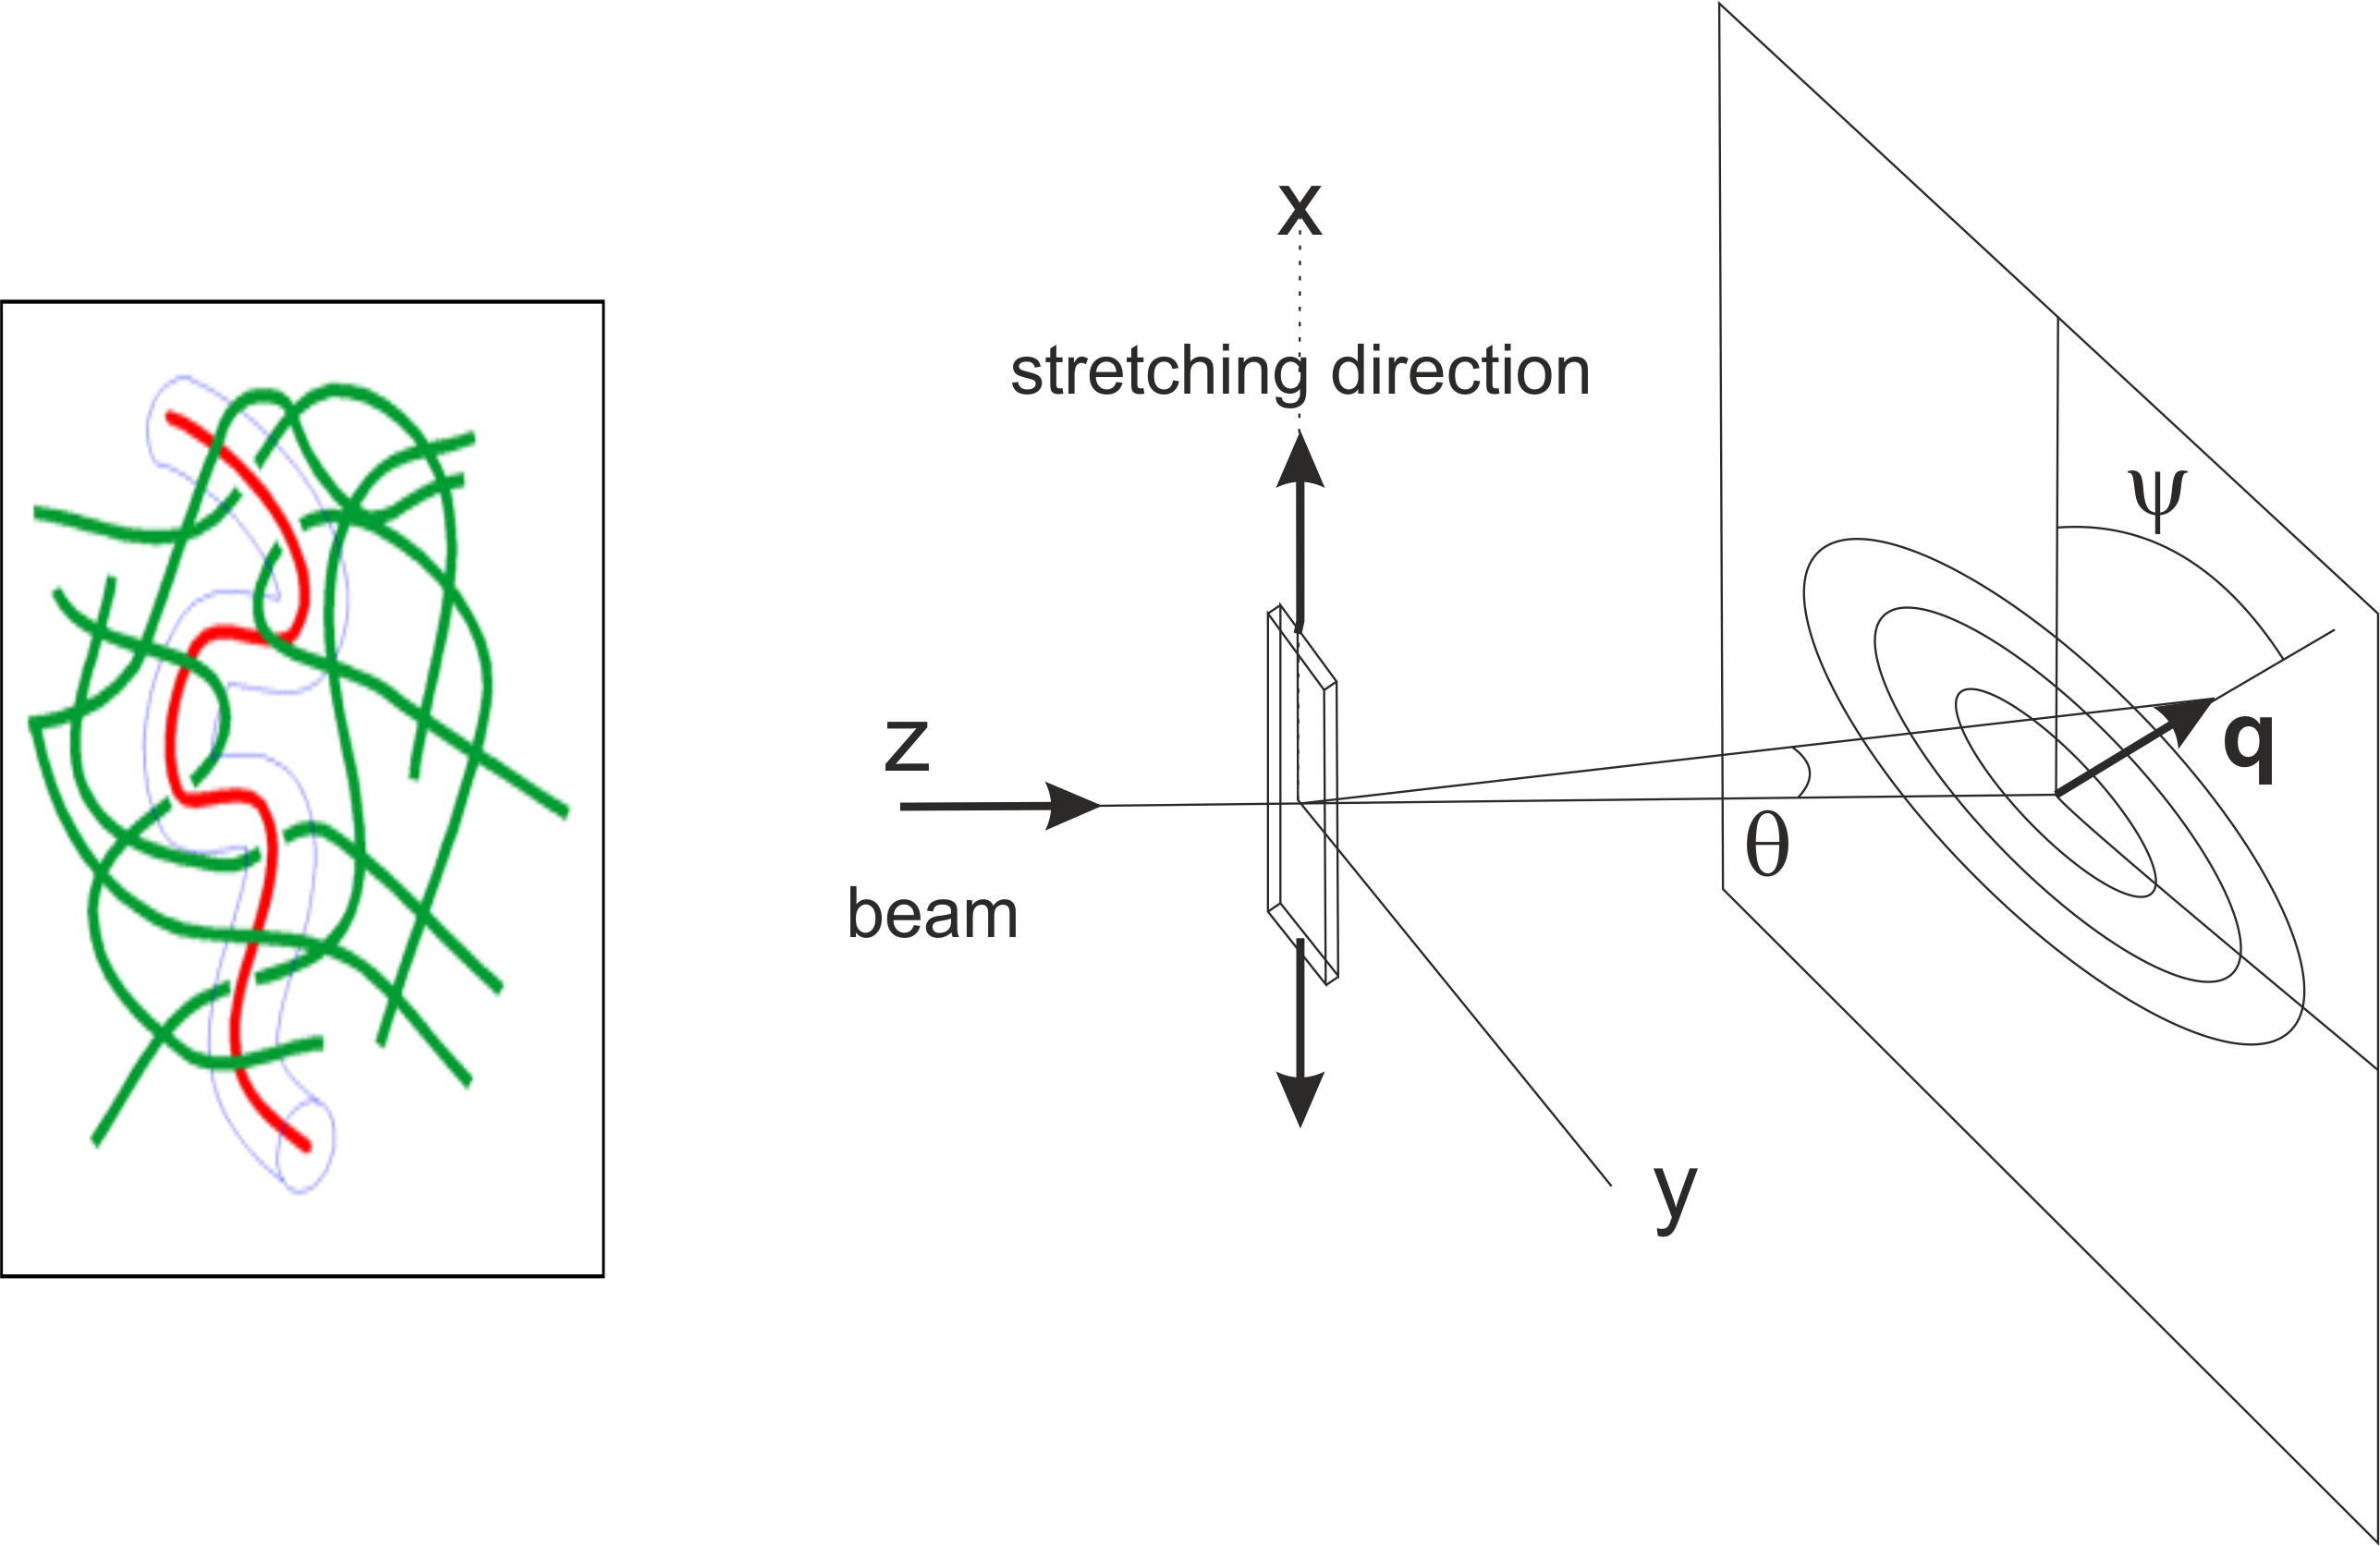
\includegraphics[width=\textwidth]{../images/form_factor/reptating_chain/reptating_chain.png}
\end{center}
\caption{Sketch of experimental setup for stretching a polymer melt.}
\label{fig:stretchpolymermelt}
\end{figure}
This model \cite{Hong1983,Noolandi1984} describes the scattering behaviour of an uniaxial deformed (stretched) Gaussian polymer chain as a function of the deformation ratio and Rouse relaxation time. The model might not include an up-to-date tube model but shows some main features of deformed polymer melts.
\newlength\breites
\settowidth\breites{$\displaystyle {}+{}$}
\begin{align}
\begin{split}
I\left(q,\frac{t}{\tau}\right)/I_0 = & \hspace{\breites}
                                        D(\alpha) + \frac{1}{6}(\alpha-\beta) \left(1+e^{-\alpha}\right) H\left(\alpha,\frac{t}{\tau}\right) \\
                                     & + \frac{1}{6}(\alpha-\beta)^2 e^{-\beta} \int_0^1 \mathrm{d}y \, y^3 e^{\beta y} \left(1+e^{-\alpha y}\right) H\left(\alpha y,\frac{t}{\tau y^2}\right)
\end{split}
\end{align}
with
\begin{align}
H\left(x,\frac{t}{\tau}\right) &= \frac{96}{\pi^2} \sum_{n = \mathrm{odd}} \frac{1}{n^2\left(n^2\pi^2+x^2\right)} e^{-n^2 \frac{t}{\tau}}
\end{align}
$D(x)$ is the Debye function $D(x) = 2\left(x - 1 + e^{-x}\right)/x^2$, $\alpha = q^2 R_g^2$, $R_g$ is the equilibrium radius of gyration
of the chain and $\tau$ is the reptation time or tube disengagement time.
Furthermore $\lambda$ is the uniaxial elongation factor, $q_\parallel$ and $q_\perp$ are respectively the components of the wave vector $q$ in directions parallel and
perpendicular to the direction of elongation which than define the parameter $\beta$ as
\begin{align}
\beta &= \left(q_\parallel^2\lambda^2+q_\perp^2/\lambda\right) R_g^2/E \\
E &= \frac{1}{2} \left\{\lambda +\frac{\mathrm{asinh}\left(\sqrt{\lambda^3-1}\right)}{\sqrt{\lambda\left(\lambda^3-1\right)}} \right\} \\
q_\parallel &= q \cos(\psi-\theta_0) \\
q_\perp &= q \sin(\psi-\theta_0)
\end{align}

\hspace{1pt}\\
\underline{Input Parameters for models \texttt{reptating chain}:}\\
\begin{description}
\item[\texttt{I0}] forward scattering $I_0$
\item[\texttt{Rg}] radius of gyration of unstretched polymer $R_g$
\item[\texttt{lambda}] stretching factor $\lambda$
\item[\texttt{t/tau}] relaxation time in units of Rouse time $t/\tau$
\item[\texttt{theta\_0}] stretching direction $\theta_0$ in the detector plane in degree
\item[\texttt{psi}] $\mathbf{q}$-direction $\psi$ in the detector plane in degree
\end{description}

\underline{Note:}
\begin{itemize}
\item The model only converges for $\lambda >1$.
\end{itemize}

\begin{figure}[htb]
\begin{center}
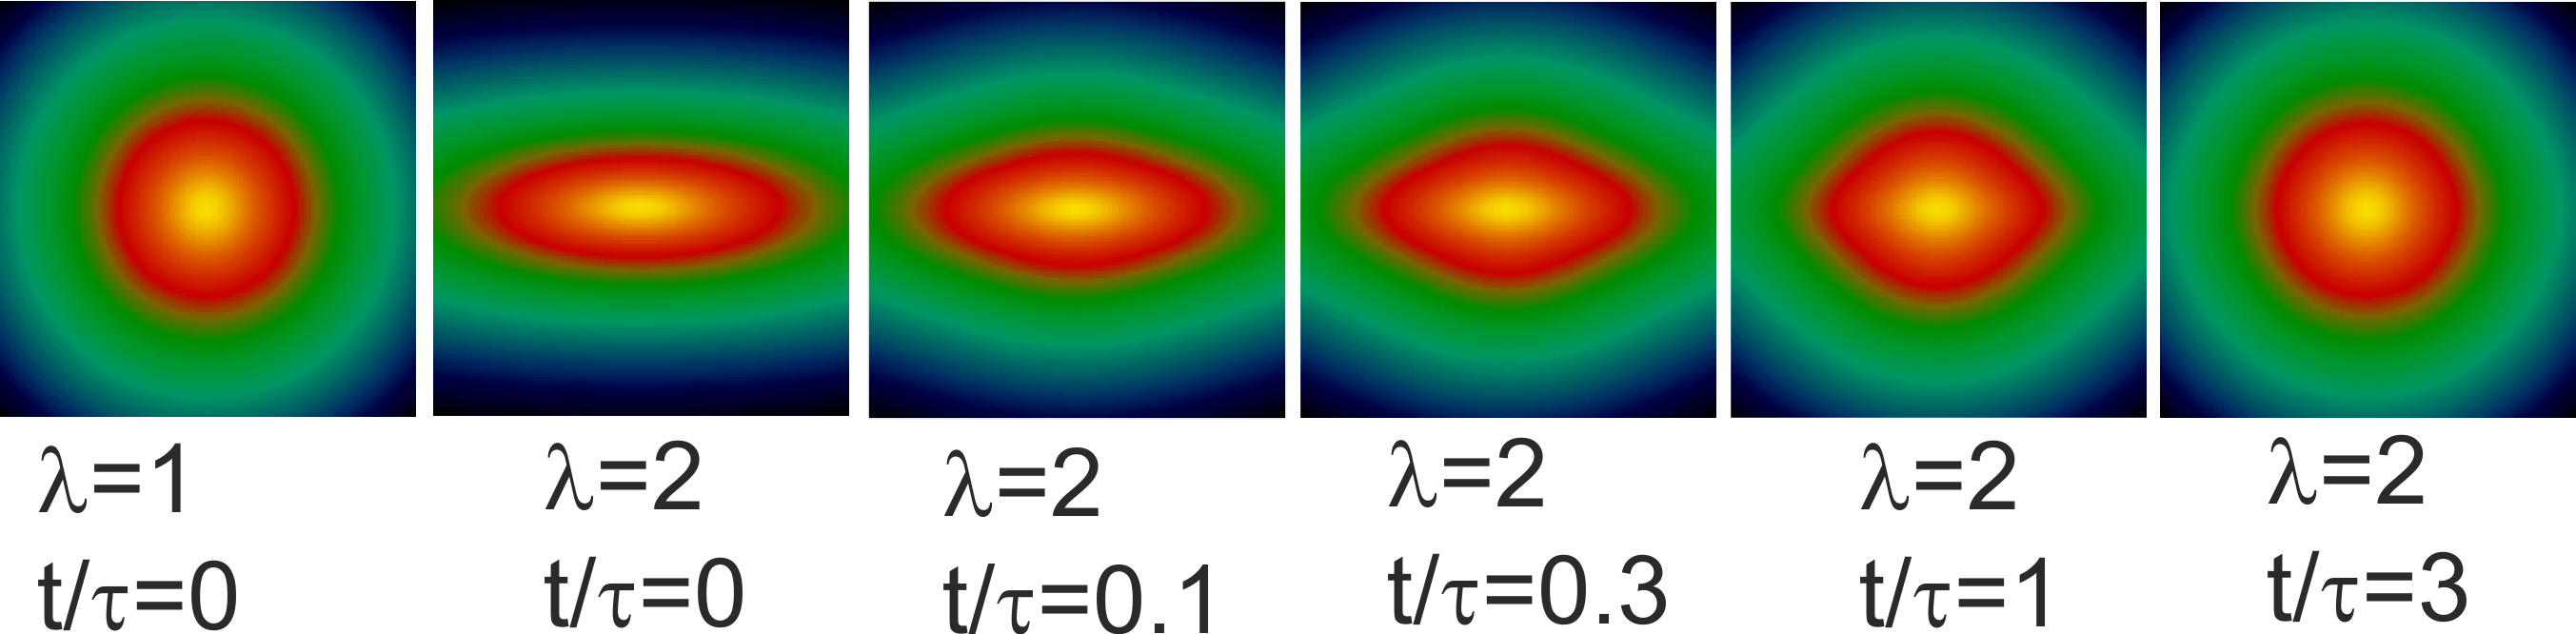
\includegraphics[width=\textwidth]{../images/form_factor/reptating_chain/lambda_2_reptating_chains.png}
\end{center}
\caption{2D scattering patterns for different relaxation times $t/\tau$ after a deformation step of $\lambda=2$}
\label{fig:IQ2Dstretchedpolymermelt}
\end{figure}

%%%%%%%%%%%%%%%%%%%%%%%%%%%%%%%%%%%%%%%%%%%%%%%%%%%%%%%%%%%%%%%%%%%%%%%%%
\newpage
\subsection{step-deformed polymer networks}
\label{sect:DeformedPolymerNetwork}
\hspace{1pt}\\
Two slightly different tube models for labeled polymer chains in a deformed network are implemented in this plugin: the original one from Warner-Edwards (WE) \cite{Warner1978} and a refined one from Heinrich-Straube-Helmis (HSH) \cite{Heinrich1988}, which have been extensively used to study uni-axial stretched polymer networks \cite{Straube1995,Mergell2001,Westermann2001,Westermann1999,Westermann1996,Read1997}.
The form factor of an uniaxial stretched polymer network with a stretching direction in the plane of the detector reads as
\begin{align}
\label{eq:SQlambda}
S(\mathbf{q},\lambda) &= \int_0^1\mathrm{d}\eta \int_0^1 \mathrm{d}\eta' \prod_{\mu} e^{-\left(Q_\mu\lambda_\mu\right)^2\abs{\eta-\eta'}-Q_\mu^2(1-\lambda_\mu^2)\xi\left\{1-\exp\left(-\frac{\abs{\eta-\eta'}}{\xi}\right)\right\}} \\
\xi &= \frac{d_\mathrm{t}^2}{2\sqrt{6}R_g^2} \\
Q_\mu &= q_\mu R_g\\
\mu  &= x,y,z \\
\mathbf{q} &= \Vek{q_x}{q_y}{q_z} = \Vek{q \cos(\psi-\delta)}{q\sin(\psi-\delta)}{0}
\end{align}
As the function of the integral kernel in eq.\ \ref{eq:SQlambda} only depends on $\abs{\eta-\eta'}$ one can transform the 2D-integral into a 1D-integral by using the identity
\begin{align}
\label{eq:2D1D_int_identity}
\int_0^1\mathrm{d}\eta \int_0^1 \mathrm{d}\eta' \: K\left(\abs{\eta-\eta'}\right) &= 2 \int_0^1 (1-x)K(x)\: \mathrm{d}x
\end{align}
The difference between the WE-model and the HSH-model is how the deformed tube diameter $d_\mathrm{t}$ is calculated. In case of the WE-model the projection $d_\mu$ of $d_t$ onto the Cartesian axis are used, whereas the HSH-model uses an effective angle dependent diameter $d_\phi$.
\begin{align}
\mbox{(WE-model): } d_\mathrm{t} &= d_\mu^2 = d_0^2\lambda_\mu^{2\nu} \\
\mbox{(HSH-model): } d_\mathrm{t} &= d_\phi^2 = d_0^2\lambda_\phi^{2\nu}
\end{align}
If we assume an elongation ratio of $\lambda$ in the $x$-direction
\begin{align}
  \lambda_x &=\lambda_{\|}=\lambda, \quad \lambda_y=\lambda_z=\lambda_\perp=\frac{1}{\sqrt{\lambda}} \\
  \lambda_\phi^2 &= \lambda_{\|}^2 \cos^2(\psi-\delta)+\lambda_\perp^2\sin^2(\psi-\delta)
\end{align}
where $R_g$ the radius of gyration of the un-deformed polymer network $\lambda_\mu$ is the macroscopic stretch ratio in this Cartesian direction and the exponent $\nu$ is predicted to take a value of $1/2$ in the case of networks \cite{Straube1995,Read2004}.  Nevertheless $\nu$ is kept as a fit parameter in this plug-in function.
\begin{multline}
\label{eq:SQ_WE_HSH}
%\begin{split}
S^\mathrm{WE}(\mathbf{q},R_g,\lambda,\nu,d_0) = \\ 2\int_0^1\mathrm{d}x\: (1-x) e^{\left(\sum_{\mu} -Q_\mu^2\lambda_\mu^2 x-
(1-\lambda_\mu^2)Q_\mu^2\xi_\mu\left\{1-e^{\left(-\frac{x}{\xi_\mu}\right)}\right\}\right)}
\end{multline}
\begin{multline}
S^\mathrm{HSH}(\mathbf{q},R_g,\lambda,\nu,d_0) = \\ 2\int_0^1\mathrm{d}x\: (1-x) e^{\left(\sum_{\mu} -Q_\mu^2\lambda_\mu^2 x- % \\ &\qquad \qquad
 (1-\lambda_\mu^2)Q_\mu^2\xi_\phi\left\{1-e^{\left(-\frac{x}{\xi_\phi}\right)}\right\}\right)}
\end{multline}
with
\begin{align}
  \xi_\mu =& \frac{d_\mu^2}{2\sqrt{6}R_g^2} \\
  \xi_\phi =& \frac{d_\phi^2}{2\sqrt{6}R_g^2}
\end{align}
In a work of \cite{Ariane2004} an additional retraction coefficient $\gamma(t)$ has been included so that the final equation for the HSH model reads as
\begin{multline}
\label{eq:SQ_HSH_retraction}
S^\mathrm{HSH}(\mathbf{q},R_g,\lambda,\nu,\gamma,d_0) =  2\int_0^1\mathrm{d}x\: (1-x) \exp\Bigg(\sum_{\mu} Q_\mu^2\left[-\lambda_\mu^2\frac{x}{\gamma(t)}- \right. \\
\left. \xi_\phi\left\{1-e^{\left(-\frac{x}{\xi_\phi\gamma(t)}\right)}\right\} +\lambda_\mu^2\xi_\phi\left\{1-e^{\left(-\frac{x}{\xi_\phi}\right)}\right\} \right]\Bigg)
\end{multline}
The retraction coefficient is for short times $\gamma(t=0)=1$ and becomes larger for increasing relaxation times $\gamma(t>0)>1$.

\begin{figure}[htb]
\begin{center}
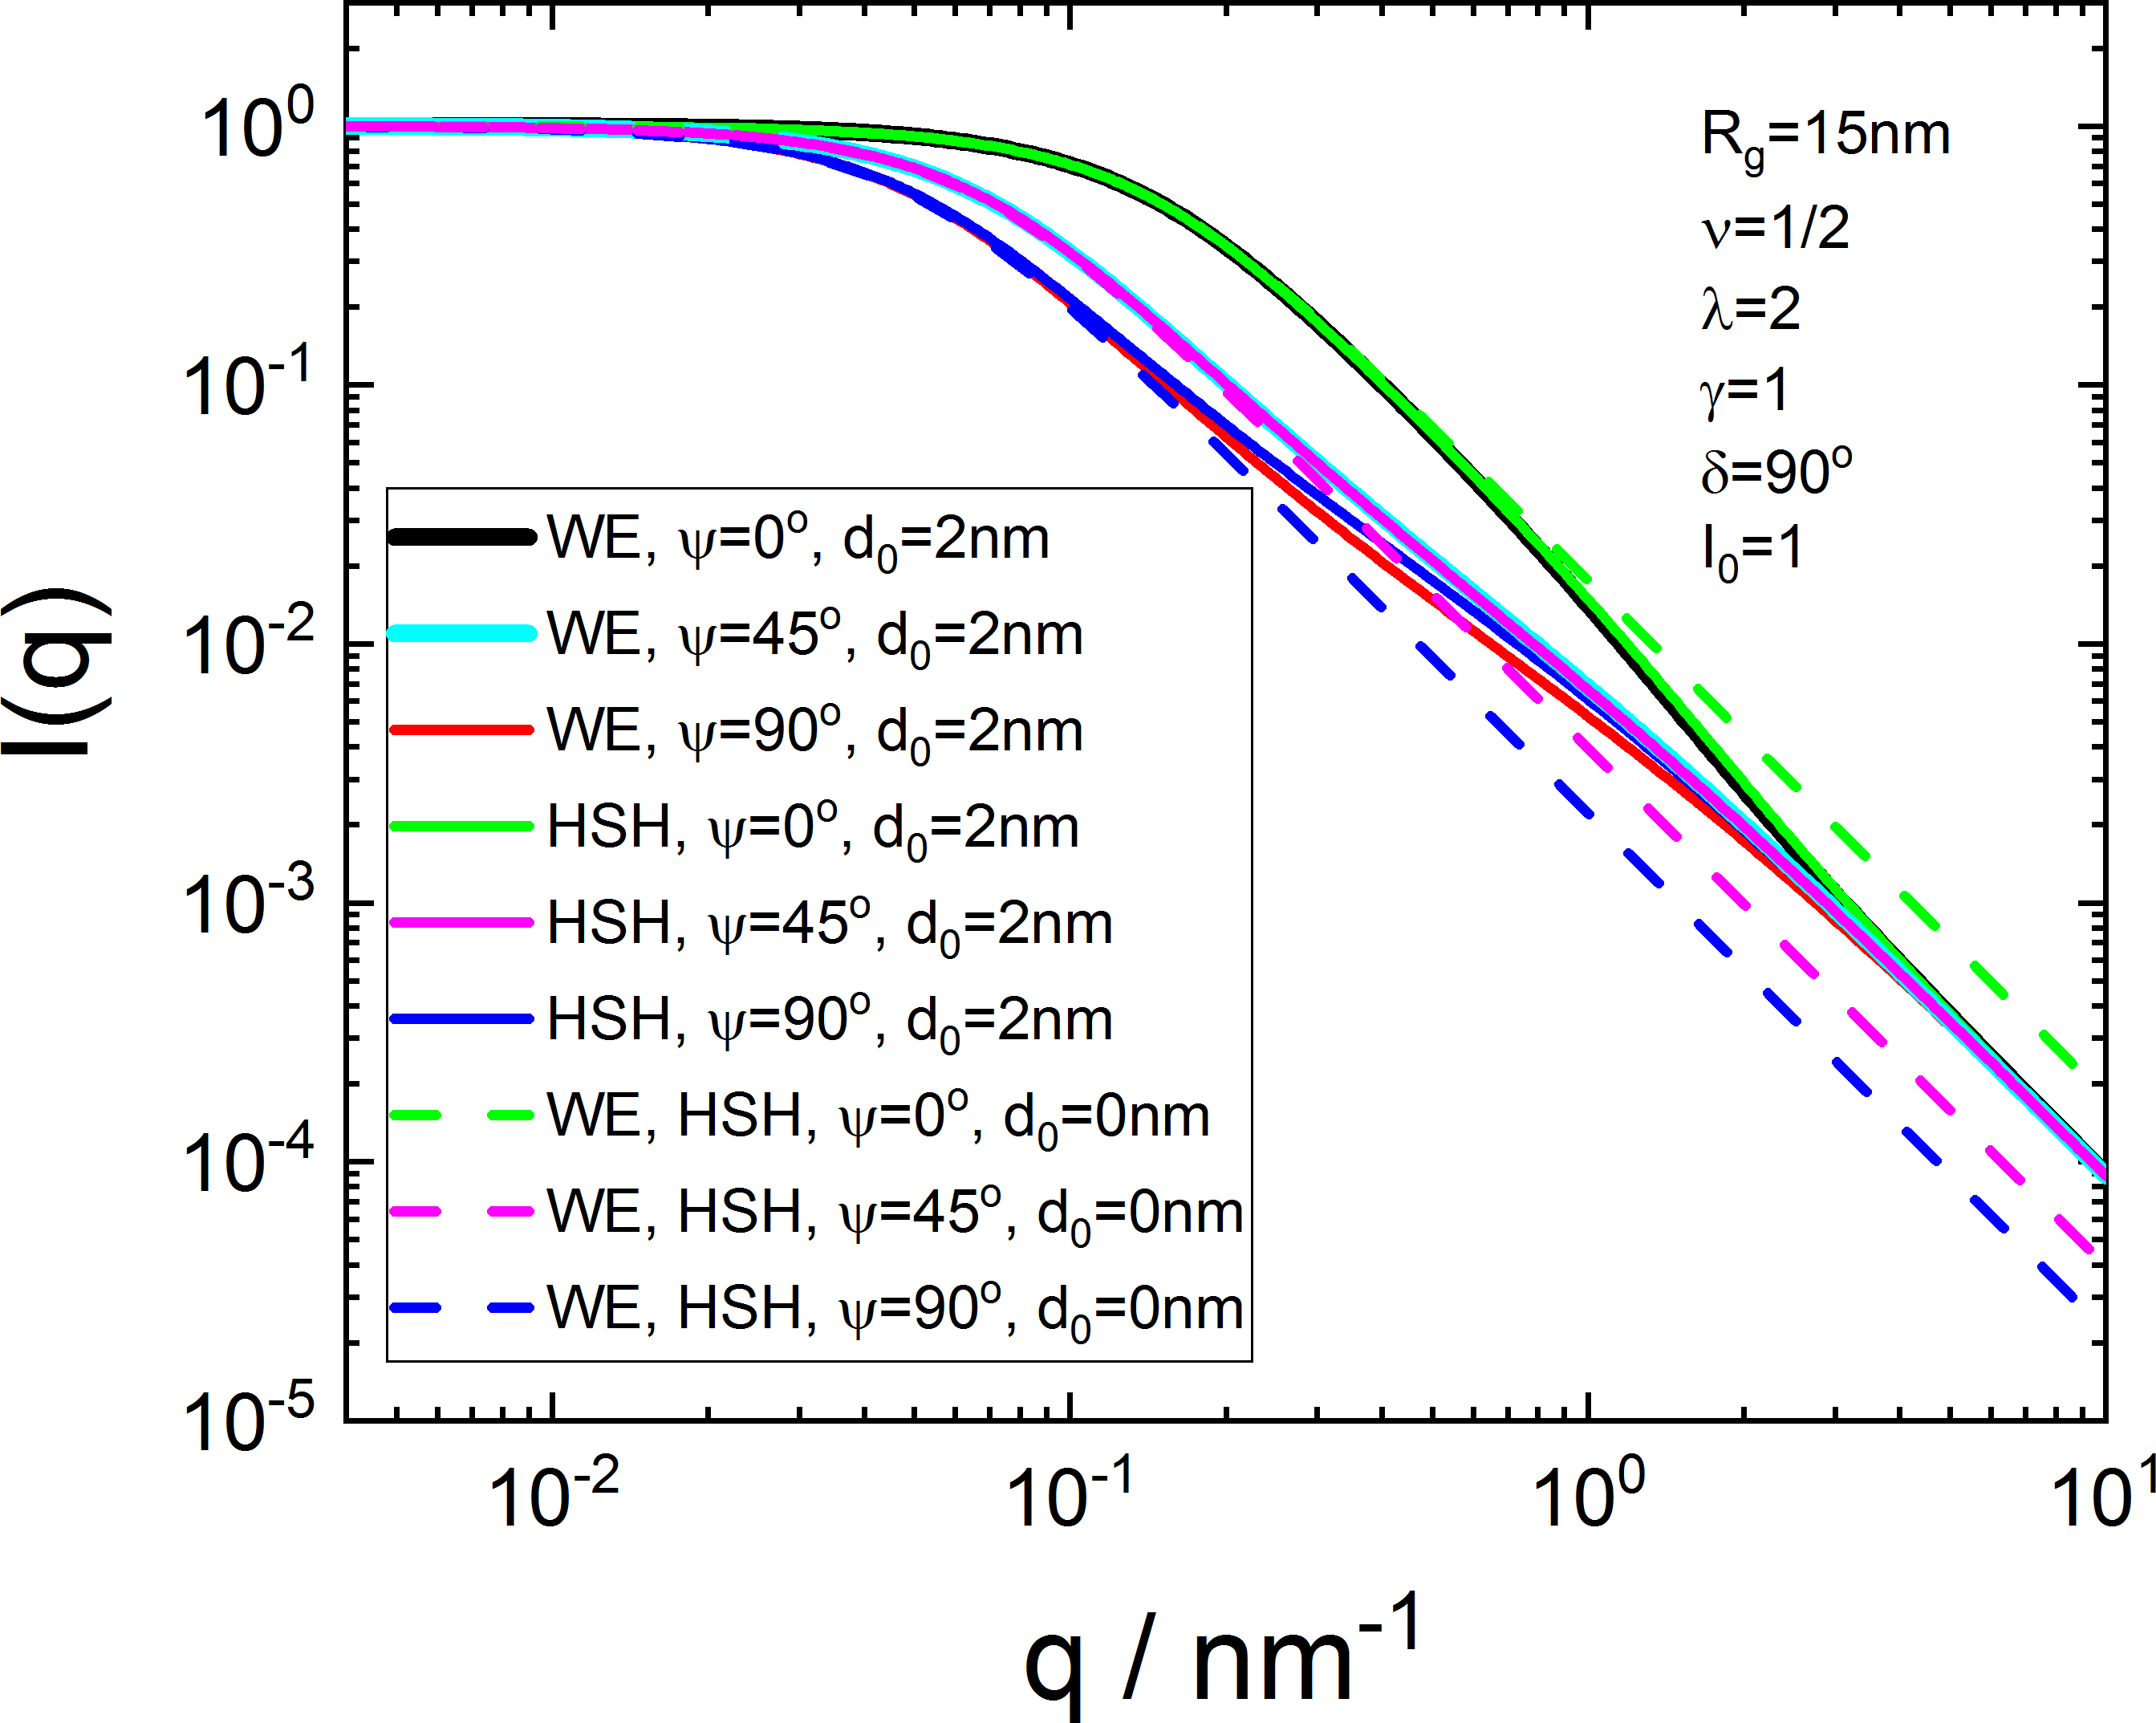
\includegraphics[width=0.7\textwidth]{../images/form_factor/deformed_sheared/deformed_polymer_network_I(sector).png}
\end{center}
\caption{sector averaged scattering curves of the Warner-Edwards and Heinrich-Straube-Helmis model of step-deformed polymer networks for tube diameters $d_0$ of 2nm and zero nm}
\label{fig:I(sector)polymernetwork}
\end{figure}

\hspace{1pt}\\
\underline{Input Parameters for models \texttt{WE: deformed polym. netw.}:}\\
\begin{description}
\item[\texttt{I0}] forward scattering $I_0$
\item[\texttt{Rg}] radius of gyration of unstretched polymer $R_g$
\item[\texttt{d0}] equilibrium tube diameter $d_0$
\item[\texttt{nu}] exponent ($\nu=1/2$, $\nu=1$:affine deformation)
\item[\texttt{lambda}] deformation ratio $\lambda$ along deformation axis
\item[\texttt{dummy}] not used
\item[\texttt{psi}] direction $\psi$ of the scattering vector $\mathbf{q}$ in the detector plane in degree
\item[\texttt{delta}] stretching direction in the detector plane $\delta$ in degree
\end{description}

\hspace{1pt}\\
\underline{Input Parameters for models \texttt{HSH: deformed polym. netw.}:}\\
\begin{description}
\item[\texttt{I0}] forward scattering $I_0$
\item[\texttt{Rg}] radius of gyration of unstretched polymer $R_g$
\item[\texttt{d0}] equilibrium tube diameter $d_0$
\item[\texttt{nu}] exponent ($\nu=1/2$, $\nu=1$:affine deformation)
\item[\texttt{lambda}] deformation ratio $\lambda$ along deformation axis

\item[\texttt{gamma}] retraction coefficient ($1 < \gamma \lesssim 2$)
\item[\texttt{psi}] direction $\psi$ of the scattering vector $\mathbf{q}$ in the detector plane in degree
\item[\texttt{delta}] stretching direction in the detector plane $\delta$ in degree
\end{description}

\underline{Note:}
\begin{itemize}
\item for large $q$-values the integration routines might fail to converge.
\end{itemize}

\begin{figure}[htb]
\begin{center}
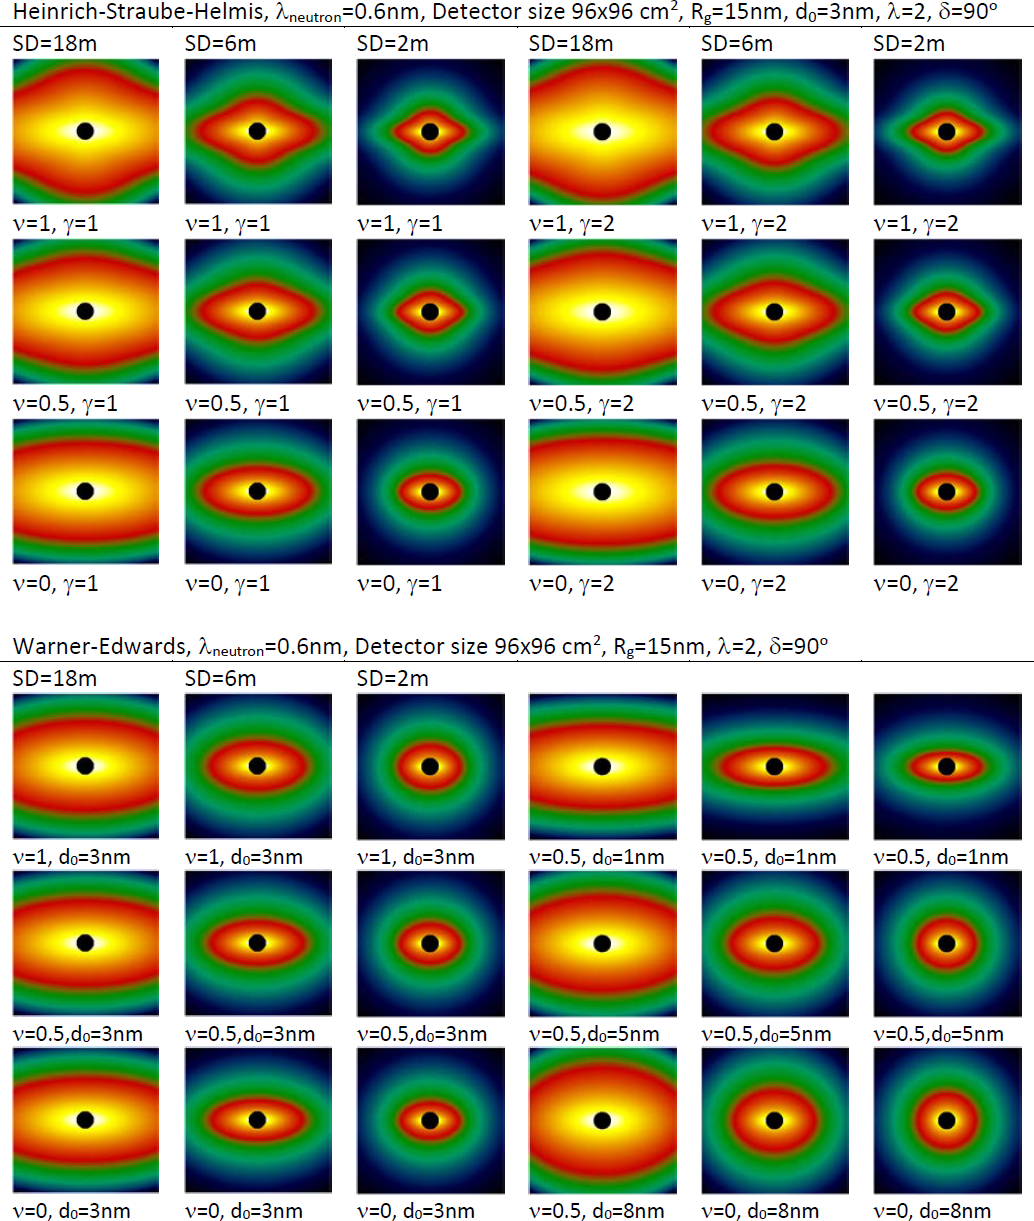
\includegraphics[width=0.7\textwidth]{../images/form_factor/deformed_sheared/deformed_polymer_network.png}
\end{center}
\caption{2D scattering patterns of the Warner-Edwards and Heinrich-Straube-Helmis model of step-deformed polymer networks}
\label{fig:IQ2Dpolymernetwork}
\end{figure}


%%%%%%%%%%%%%%%%%%%%%%%%%%%%%%%%%%%%%%%%%%%%%%%%%%%%%%%%%%%%%%%%%%%%%%%%%
\newpage
\subsection{linear polymer under shear flow}~\\
\label{sect:LinearPolymerShearFlow}
The form factors describing linear polymers under shear flow has been taken from \cite{Korolkovas2019}.
It is assumed that the shear-vorticity plane is the same than the detector plane. In the paper three models are given. In the continuous limit the form factor is given by a double integral
\begin{align}
  P(\mathbf{q}) & = \frac{1}{N^2}\int_0^N\mathrm{d}n\int_0^N\mathrm{d}m\: \exp\left(-\frac{\langle(\mathbf{q}\cdot\mathbf{r}_{nm})^2\rangle}{2}\right)
\end{align}
In all three cases given in that paper the mean squared displacement function (MSD) $\langle(\mathbf{q}\cdot\mathbf{r}_{nm})\rangle/2$ was supplied as a function of $x=\abs{n-m}/N$, which in the end allows to replace the double integral by a single integral.
\begin{align} \label{eq:IQ_MSD}
 P(\mathbf{q}) & = 2\int_0^1 (1-x) \exp\left(-\frac{\langle(\mathbf{q}\cdot\mathbf{r}_{nm})^2\rangle}{2}\right) \mathrm{d}x
\end{align}
\begin{itemize}
\item In equilibrium an exact solution of that integral is available as in this case
\begin{align}
  \frac{\langle(\mathbf{q}\cdot\mathbf{r}_{nm})^2\rangle}{2} & = a \abs{n-m}/N
\end{align}
with $N$ being the number of segments of the polymer, $a=(qR_g)^2=N\lambda^2/6$, where $\lambda$ is the Kuhn length and $R_g$  the equilibrium radius of gyration, so that
\begin{align}
  P_\mathrm{iso}(\mathbf{q}) & = \frac{2\left(e^{-a}-1+a\right)}{a^2}
\end{align}
\item for the polymer under shear flow they approximated the MSD-function as a series of straight lines. In the case of two linear segments the MSD function reads as
    \begin{align}
      \frac{\langle(\mathbf{q}\cdot\mathbf{r}_{nm})^2\rangle}{2} &=
      \begin{cases}
        b\abs{n-m}/N, & \mbox{if } \abs{n-m}/N \leq \nu \\
        c\abs{n-m}/N+(b-c)\nu, & \mbox{otherwise}.
      \end{cases}
    \end{align}
    with $0<(\nu<N_1/N)<1$. To account for the deformation of the polymer $b$ and $c$ are described by
    \begin{align}
      b &= R_g^2\left[(\alpha q \cos^2(\psi-\phi_0))+(\beta q \sin^2(\psi-\phi_0))\right] \\
      c &= R_g^2\left[(\gamma q \cos^2(\psi-\phi_0))+(\delta q \sin^2(\psi-\phi_0))\right]
    \end{align}
    which gives four fitting parameters $(\alpha,\beta,\gamma,\delta)$. $R_g$ is the equilibrium radius of gyration, $\psi$ the direction if the scattering vector in the detector plane and $\phi_0$ the flow-direction. The form factor can be calculated also analytical and is given by
    \begin{align}
      P(\mathrm{q}) & = \frac{2}{b^2}\left(b-1+e^{-\nu b} \left\{1+\left[\frac{b^2}{c^2}-1\right]e^{(\nu-1)c}+
                        (1-\nu)\frac{b}{c}(b-c)\right\}\right)
    \end{align}
\item  a semi-empirical 3-parameter formula $(B_x,B_y,\xi)$ to have a similar shape than the piecewise linear MSD function above.
    \begin{multline}
    \frac{\langle(\mathbf{q}\cdot\mathbf{r}_{nm})^2\rangle}{2} =\left(qR_g\right)^2 \times \\
    \left\{
      \abs{\frac{n-m}{N}} + \left[B_x^2\cos^2(\psi-\phi_0)-B_y^2\sin^2(\psi-\phi_0)\right]\abs{\frac{n-m}{N}}^\xi
    \right\}
    \end{multline}
    To get the same endpoints than the piecewise linear MSD function the amplitudes should be $B_x=\sqrt{\nu\alpha^2+(1-\nu)\gamma^2}$ and $B_y=\sqrt{\nu\beta^2+(1-\nu)\delta^2}$.
    After making use of the identity \ref{eq:2D1D_int_identity} the scattering intensity is than given by
    \begin{multline}
      P(\mathbf{q}) = 2 \int_0^1 (1-x) \exp\Bigg( \left(qR_g\right)^2\\
      \left(
      x + \left(B_x^2q^2\cos^2(\psi-\phi_0)+B_y^2q^2\sin^2(\psi-\phi_0)\right)x^\xi
      \right)\Bigg)
    \end{multline}
\item by applying the Rouse model \cite{Korolkovas2019} the MSD which reads as
    \begin{multline}\label{eq:MSDlinearShearFlow}
    \frac{\langle(\mathbf{q}\cdot\mathbf{r}_{nm})^2\rangle}{2} = \left(qR_g\right)^2 \times \\ \left[ x+\frac{\left(\cos(\psi-\phi_0)\pi^2\operatorname{Wi}_\mathrm{lin}\right)^2}{180} x^2\left(1+x-x^2/4-2x^3+x^4\right) \right]
    \end{multline}
    with $x=\abs{\frac{n-m}{N}}$ and the Weissenberg number $\operatorname{Wi}_\mathrm{lin}=\tau_1\dot{\gamma}$.
\end{itemize}

\subsection{ring polymer under shear flow}~\\
Ring polymers under shear flow also can be described using the Rouse model \cite{Tsolou2010,Stephanou2019} similarly to eq.\ \ref{eq:MSDlinearShearFlow}. The mean square displacement then reads as
\begin{align}\label{eq:MSDringShearFlow}
\frac{\langle(\mathbf{q}\cdot\mathbf{r}_{nm})^2\rangle}{2} &= 2\left(qR_{g,\mathrm{ring}}\right)^2
\left[ \mu+\frac{\left(\cos(\psi-\phi_0)\pi^2\operatorname{Wi}_\mathrm{ring}\right)^2}{1440} \left(\mu^2+2\mu^3\right) \right]
\end{align}
with $\mu=x(1-x)$, $x=\abs{\frac{n-m}{N}}$, $\operatorname{Wi}_\mathrm{ring}=\tau_1\dot{\gamma}$, and $R_{g,\mathrm{ring}}^2=\frac{Nb^2}{12}=R_{g,\mathrm{lin}}^2/2$. The scattering intensity is then obtained by eq.\ \ref{eq:IQ_MSD}
\begin{align}
 P(\mathbf{q}) & = 2\int_0^1 (1-x) \exp\left(-\frac{\langle(\mathbf{q}\cdot\mathbf{r}_{nm})^2\rangle}{2}\right) \mathrm{d}x
\end{align}
%%%%%%%%%%%%%%%%%%%%%%%%%%%%%%%%%%%%%%%%%%%%%%%%%%%%%%%%%%%%%%%%%%%%%%%%%
\newpage
\subsection{Sheared Cylinder according to Hayter and Penfold}
\label{sect:ShearedCylinderHayterPenfold}
\hspace{1pt}\\
The orientation distribution of long cylinders in a shear cell has been studied by \cite{Scheraga1951,Jerrard1959,Hayter1984}. In contrast to the orientation distributions described in the next section this distribution also describes the tilting of the most probable orientation against the flow direction.
\begin{figure}[htb]
\begin{center}
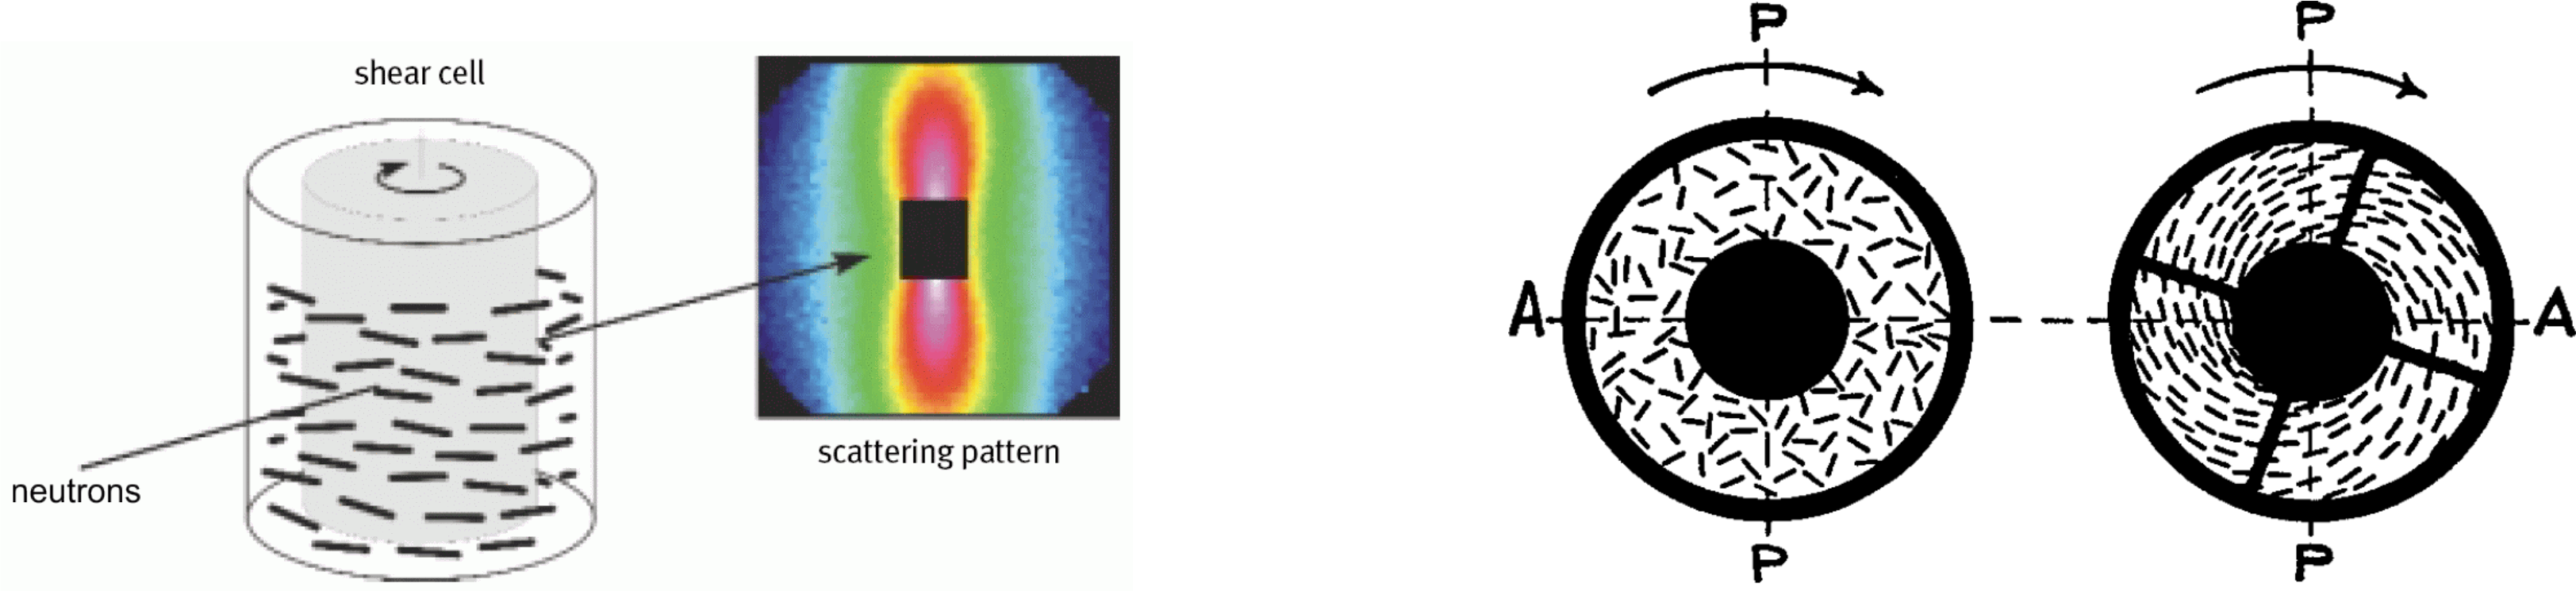
\includegraphics[width=\textwidth]{sheared_cylinders_n_phi0.png}
\end{center}
\caption{Shear orientation of micelles in a shear cell with the
corresponding SANS-pattern. The orientation of rods at rest and under shear according to \cite{Scheraga1951} are shown on th e right as a top view on the cuette cell.} \label{sheared_cylinders1}
\end{figure}

\begin{figure}[htb]
\begin{center}
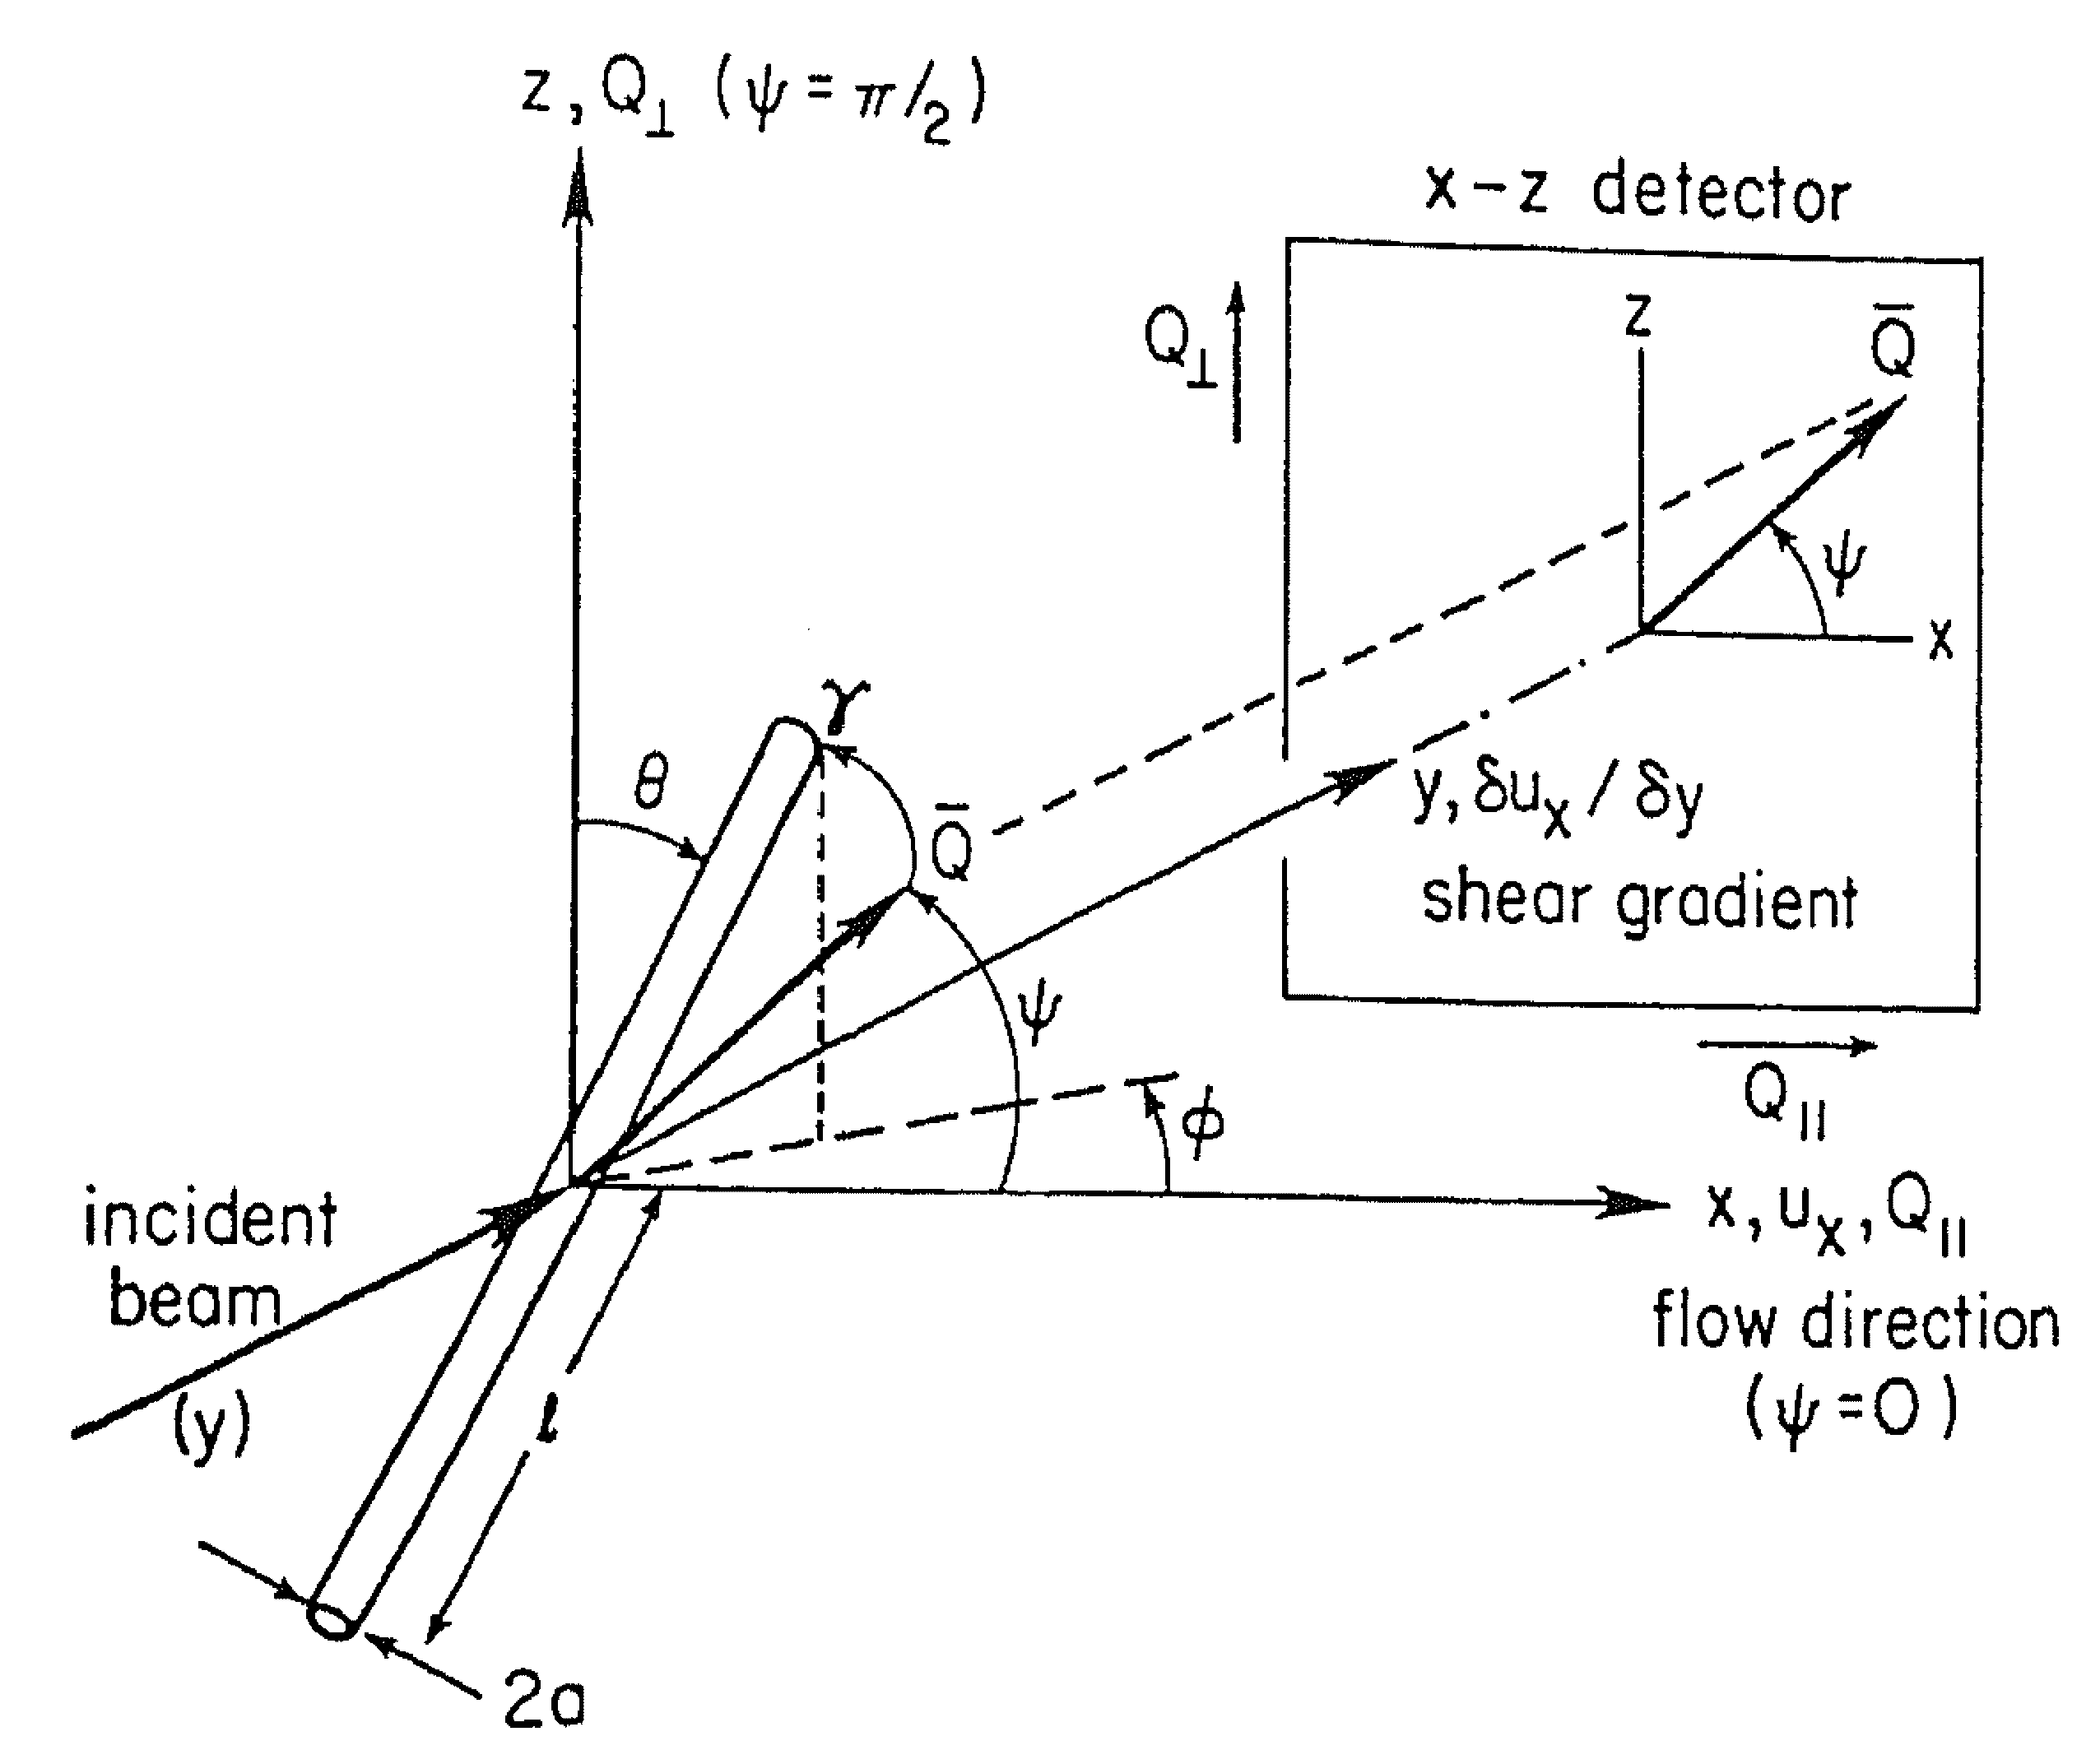
\includegraphics[width=0.7\textwidth]{shear_cuette_SANS_geometry.png}
\end{center}
\caption{Cartesian and angular coordinates referred to the center
of a cylindrical micelle at origin \cite{Hayter1984}. The relationship to the
spectrometer geometry is shown schematically. The momentum
transfer, $Q$, lies in the $z-x$ plane.}
\label{shear_cuette_SANS_geometry}
\end{figure}

The scattering from monodisperse dilute (non-interacting)
isotropic solution of anisotropic micelles is given by \cite{Hayter1984}
\BE
I(Q) =
\left< \vert K_\text{CylSh}(Q)\vert^2 \right>_Q \label{IQ_av}
\EE
where $K(Q)$
is the form factor for a micelle at a given orientation relative
to the momentum transfer $Q$ and $\left<\right>_Q$ denotes an
average over all such orientations.


For a cylindrical shell of length $L$, core diameter $2R$, and shell thickness $t$ the form
factor is given by:
\begin{align}
\begin{split}
K_\text{CylSh}\left(Q,\dots,\gamma\right)  = &
                  \hspace{\breites} K_\text{Cyl}\left(Q,\eta_\text{core}-\eta_\text{shell},R,L,\gamma\right) \\
                               & +  K_\text{Cyl}\left(Q,\eta_\text{shell}-\eta_\text{solv},R+\Delta R,L,\gamma\right)
\end{split}
\end{align}
with
\begin{align}
K_\text{Cyl}(Q,\Delta\eta,R,L,\gamma) & = 2 \pi R^2 L \Delta \eta
    \frac{J_1\left(Q R \sin\gamma\right)}{Q R \sin\gamma} \,
    \frac{\sin\left(\frac{QL}{2} \cos\gamma\right)}{\frac{QL}{2} \cos\gamma}
\end{align}
where $\gamma$ is the angle between $\mathbf{Q}$ and the cylinder
axis $\mathbf{n}$. $\eta_\text{core}$, $\eta_\text{shell}$, and $\eta_\text{solv}$ are the scattering length densities of the cylinder core, shell and solvent. $J_1(x)$ is the first order Bessel function of
the first kind. $\gamma$ can be calculated from the orientation
($\theta$, $\phi$) of the cylinder and the direction of the
scattering vector $\psi$ in the plane of the detector by
where $\gamma$ is the angle between $Q$ and the cylinder axis.

The scattering geometry for shear alignment is shown in Fig.
\ref{shear_cuette_SANS_geometry}. In general perfect alignment
will not be achieved, and an orientation distribution must be
employed such that the resultant scattering will be given by
\begin{align}
I(Q,\psi) &= \int_0^{2\pi} \int_0^\pi
p_\mathrm{HP}(\theta,\phi;\kappa)\, \left(K^2_\text{CylSh}(Q,\gamma^+)+K^2_\text{CylSh}(Q,\gamma^-)
\right) \sin\theta \mathrm{d}\theta \mathrm{d}\phi
\label{eq:IQShear_pHP}
\end{align}
with
\begin{align}
p_\mathrm{HP}(\theta,\phi;\kappa) & = \frac{(1-\cos
2\varPhi_0)(1+\sin^2\theta\cos 2\varPhi_0)^{3/2}}{4\pi\left[
1-\sin^2\theta\cos 2\varPhi_0\cos 2(\phi-\varPhi_0)\right]^2}
\end{align}
and
\BE
2\varPhi_0 = \arctan(8/\kappa)
\EE
$(\cos \varPhi_0,\sin \varPhi_0,0)^T$
is the direction of the most probable orientation $(\theta=\frac{\pi}{2};\phi=\varPhi_0)$. $\varPhi_0$ varies between $\varPhi_0=\frac{\pi}{4}$ for the isotropic case ($\kappa=0$)  to $\varPhi_0=0$ for perfect alignment ($\kappa\rightarrow \infty$).
\begin{figure}[htb]
\begin{center}
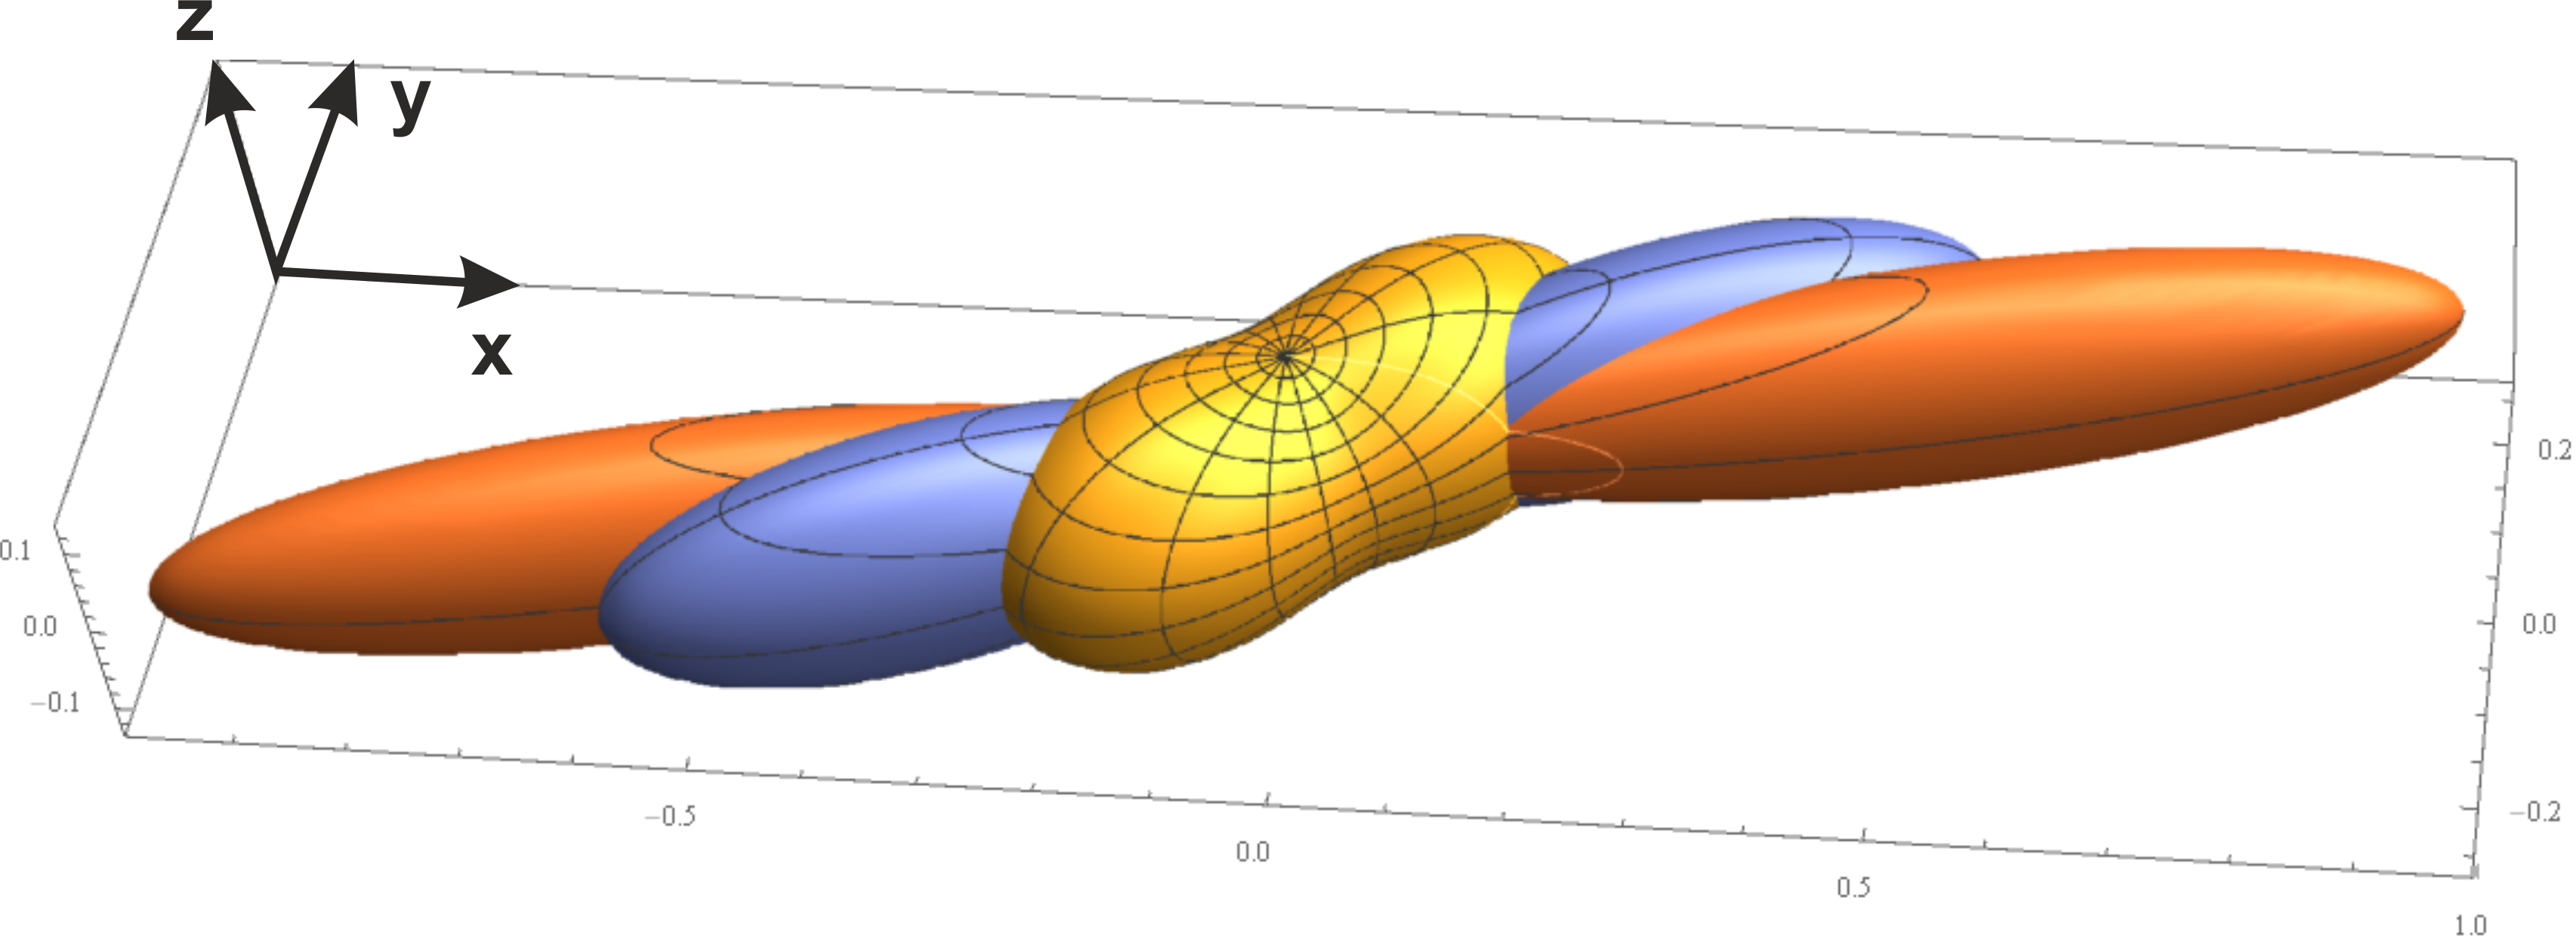
\includegraphics[width=\textwidth]{../images/form_factor/cylindrical_obj/pHP3D.png}
\end{center}
\caption{3D plot of the orientation distributions $2 p_\mathrm{HP}(\theta,\phi;\kappa={2})$ ({\bf \color[rgb]{1.0, 0.85, 0.0}yellow}), $p_\mathrm{HP}(\theta,\phi;\kappa{=}8)$ ({\bf\color[rgb]{0.36, 0.57, 0.9} blue}), $\frac12 p_\mathrm{HP}(\theta,\phi;\kappa{=}16)$ ({\bf\color[rgb]{1.0, 0.5, 0.0} orange}).} \label{fig:pHP3D}
\end{figure}
As the most probable direction is not the same as the flow direction, which is assumed to be the $x$-direction, and secondly that the beam is passing twice the cuette cell with flow direction $\mathbf{x}$ and $-\mathbf{x}$ we have to take the sum over two values for $\gamma^\pm$ in eq.\ \ref{eq:IQShear_pHP}. The angle $\gamma^\pm = \angle(\mathbf{Q,n}^\pm)$ between the scattering vector $\mathbf{Q}$ and the director of the cylinder axis $\mathbf{n}^\pm$ is
\begin{align}
\frac{\mathbf{Q}}{\abs{\mathbf{Q}}} &=
\begin{pmatrix}
\cos \psi \\
0  \\
\sin \psi
\end{pmatrix} \qquad
\frac{\mathbf{n}^\pm}{\abs{\mathbf{n}^\pm}} =
\begin{pmatrix}
\pm \sin \theta \cos \phi \\
\pm \sin \theta \sin \phi  \\
\cos \theta
\end{pmatrix} \\
\cos \angle(\mathbf{Q,n}^\pm) &= \cos \gamma^\pm = \frac{\mathbf{Q\cdot n}^\pm}{\abs{\mathbf{Q}}\abs{\mathbf{n}^\pm}} =  \pm \cos\psi \sin\theta \cos\phi + \sin\psi \cos\theta
\end{align}
For the reversed direction of the flow the $x$-component of the vector $\mathbf{n}^-$ changes its sign. In the original paper \cite{Hayter1984} one finds $\cos \gamma^-_\mathrm{HP} = \cos\psi \sin\theta \cos\phi - \sin\psi \cos\theta$, which, however, results to the same scattering intensity as the scattering intensity of a cylinder is invariant by a rotation of $\pi$, i.e. as $\cos(\pi+\gamma^-) =-\cos\gamma^- = \cos\gamma^-_\mathrm{HP}$ the resulting scattering patterns are the same for both value $\gamma^-$ and $\gamma^-_\mathrm{HP}$.

\vspace{5mm}

\underline{Input Parameters for model \texttt{Sheared Cylinders (HayterPenfold)}:}\\
\begin{description}
\item[\texttt{R}] radius of cylinders $R$
\item[\texttt{t}] shell thickness $t$
\item[\texttt{L}] cylinder length $L$
\item[\texttt{eta\_core}] scattering length density of cylinder core $\eta_\mathrm{core}$
\item[\texttt{eta\_shell}] scattering length density of cylinder shell $\eta_\mathrm{shell}$
\item[\texttt{eta\_solv}] scattering length density of solvent $\eta_\mathrm{solv}$
\item[\texttt{psi}] direction of scattering vector on the detector $\psi$
\item[{\texttt{sigma}}] width parameter of lognormal size distribution $\sigma$
\item[{\texttt{kappa}}] orientation distribution parameter $\kappa$
\end{description}

\underline{Note:}
\begin{itemize}
\item The size distribution is taken simultaneously over all parameters $R$, $t$ and $L$, so that their aspect rations stay always constant
\item The most probable orientation is not the $\mathbf{x}$-direction but tilted by the angle $\varPhi_0$. As in a rheometer with cuette geometry the beram is passing the sample twice the forward scattering is twice as large as in the model described in the next section.
\item As the orientation distribution is also not rotational symmetric around the direction of the most probably orientation and additional tilted against $\mathbf{x}$-axis the scattering pattern look less anisotropic than the other models in the following sections with the same order parameter $\kappa$.
\end{itemize}

%%%%%%%%%%%%%%%%%%%%%%%%%%%%%%%%%%%%%%%%%%%%%%%%%%%%%%%%%%%%%%%%%%%%%%%%%%%%%%%%%%
\newpage
\subsection{partly aligned anisotropic objects}
\label{sect:partlyalignedCylShell}
~\\

In contrast to the model of Hayter and Penfold \cite{Hayter1984} in section \ref{sect:ShearedCylinderHayterPenfold} here we use an orientation distribution with the most probably orientation along the $\mathrm{x}$-axis and independent on the polar angle $\phi$.
Therefore the coordination system is slightly differently defined in the Hayter-Penfold model of sheared cylinders.
\begin{figure}[htb]
\begin{center}
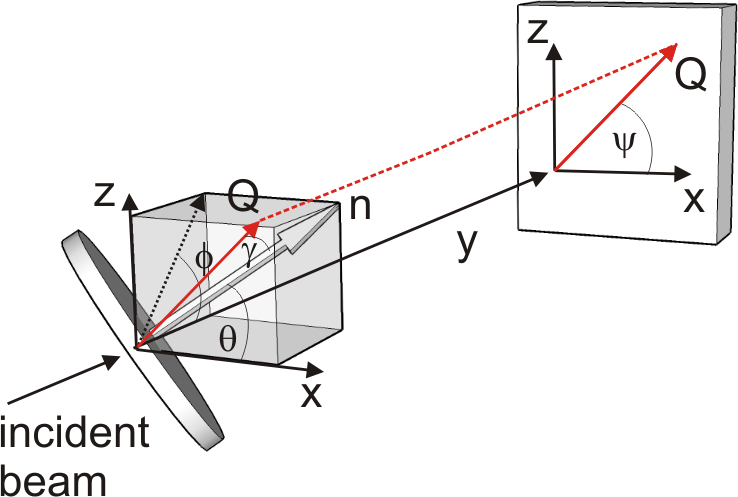
\includegraphics[width=0.7\textwidth]{../images/form_factor/cylindrical_obj/partly_aligned_discs.png}
\end{center}
\caption{Sketch of relative orientation $\mathbf{n}$ of partly
aligned cylinders or discs to the scattering vector $\mathbf{Q}$.}
\label{fig:partly_aligned_discs}
\end{figure}

\noindent The scattering amplitude of a cylindrical shell is given by
\begin{align}
\begin{split}
K_\text{CylShell}\left(Q,\dots,\gamma\right)  = &
\hspace{\breites} K_\text{Cyl}\left(Q,\eta_\text{core}-\eta_\text{shell},R,L,\gamma\right) \\
             & +  K_\text{Cyl}\left(Q,\eta_\text{shell}-\eta_\text{solv},R+\Delta R,L,\gamma\right)
\end{split}
\end{align}
with
\begin{align}
K_\text{Cyl}(Q,\Delta\eta,R,L,\gamma) & = 2 \pi R^2 L \Delta \eta
    \frac{J_1\left(Q R \sin\gamma\right)}{Q R \sin\gamma} \,
    \frac{\sin\left(\frac{QL}{2} \cos\gamma\right)}{\frac{QL}{2} \cos\gamma}
\end{align}
where $\gamma$ is the angle between $\mathbf{Q}$ and the cylinder
axis $\mathbf{n}$. $L$ is the length of the cylinder, $R$ its
radius, $\Delta\eta$ the scattering length density contrast relative
to the solvent and $J_1(x)$ is the first order Bessel function of
the first kind.

The scattering amplitude of an ellispoid of revolution is given by
\begin{align}
K_\text{Ell}(Q,\Delta\eta,R_\mathrm{e},R_\mathrm{p},\gamma) & = 4\pi R_\mathrm{e}^2 R_{p} \Delta\eta \frac{j_1(Qs)}{Qs}
\end{align}
with $s = \sqrt{R_\mathrm{p}\cos^2\gamma + R_\mathrm{e}\sin^2\gamma}$ and $j_1(x)$ being the spherical bessel function of first kind. $R_\mathrm{e}$ and $R_{p}$ are the equatorial and polar semi-axes of the spheroid, respectively.
The scattering amplitude of an ellipsoidal shell is given by
\begin{align}
\begin{split}
K_\text{EllShell}\left(Q,\dots,\gamma\right)  = &
\hspace{\breites} K_\text{Ell}\left(Q,\eta_\text{core}-\eta_\text{shell},R_{\mathrm{p}},R_{\mathrm{e}},\gamma\right) \\
             & +  K_\text{Ell}\left(Q,\eta_\text{shell}-\eta_\text{solv},R_{\mathrm{p}}+\Delta R,R_{\mathrm{e}}+\Delta R,\gamma\right)
\end{split}
\end{align}
$\gamma$ can be calculated from the orientation
($\theta$, $\phi$) of the cylinder and the direction of the
scattering vector $\psi$ in the plane of the detector by
\begin{align}
\frac{\mathbf{Q}}{\abs{\mathbf{Q}}} &=
\begin{pmatrix}
\cos \psi \\
0  \\
\sin \psi
\end{pmatrix} \qquad
\frac{\mathbf{n}}{\abs{\mathbf{n}}} =
\begin{pmatrix}
\cos \theta \\
\sin \theta \cos \phi  \\
\sin \theta \sin \phi
\end{pmatrix} \\
\cos \measuredangle(\mathbf{Q,n}) &= \cos \gamma = \frac{\mathbf{Q\cdot
n}}{\abs{\mathbf{Q}}\abs{\mathbf{n}}} = \cos\psi \cos\theta +
\sin\psi \sin\theta \sin\phi
\end{align}
If the orientation distribution of the orientation vector $\mathbf{n}$ is described by $p(\theta,\phi,\kappa)$
so that the scattering intensity is given by
\begin{align}
I_\mathrm{p.a.CylShell}(Q) & =
            \int_0^\pi d\theta \int_0^{2\pi} d\phi \, \,
                K^2_\text{CylShell}\left(Q,\dots,\gamma\right)\,p(\theta,\phi;\kappa)\,\sin(\theta) \\
I_\mathrm{p.a.EllShell}(Q) & =
            \int_0^\pi d\theta \int_0^{2\pi} d\phi \, \,
                K^2_\text{EllShell}\left(Q,\dots,\gamma\right)\,p(\theta,\phi;\kappa)\,\sin(\theta)
\end{align}
For this form factor it is assumed that the orientation distribution is independent of $\phi$,
i.e. $p(\theta,\phi;\kappa)=p(\theta;\kappa)$ and that $p(\theta;\kappa)=p(\pi-\theta;\kappa)$, which means that turning the cylinder by 180$^\circ$ results in the same scattering intensity.
Several orientation distributions have been implemented in a way that their resulting order parameter $S_2$ can have values between -0.5 and 1, which correspond to perfect alignment perpendicular to the $\mathrm{x}$ axis and perfect alignment parallel to it. All probability distributions have been normalized
\begin{align}
\int_0^\pi \int_0^{2\pi} p(\theta,\phi;\kappa) \sin \theta \, d\theta \, d\phi&=1
\end{align}
\begin{figure}[htb]
\begin{center}
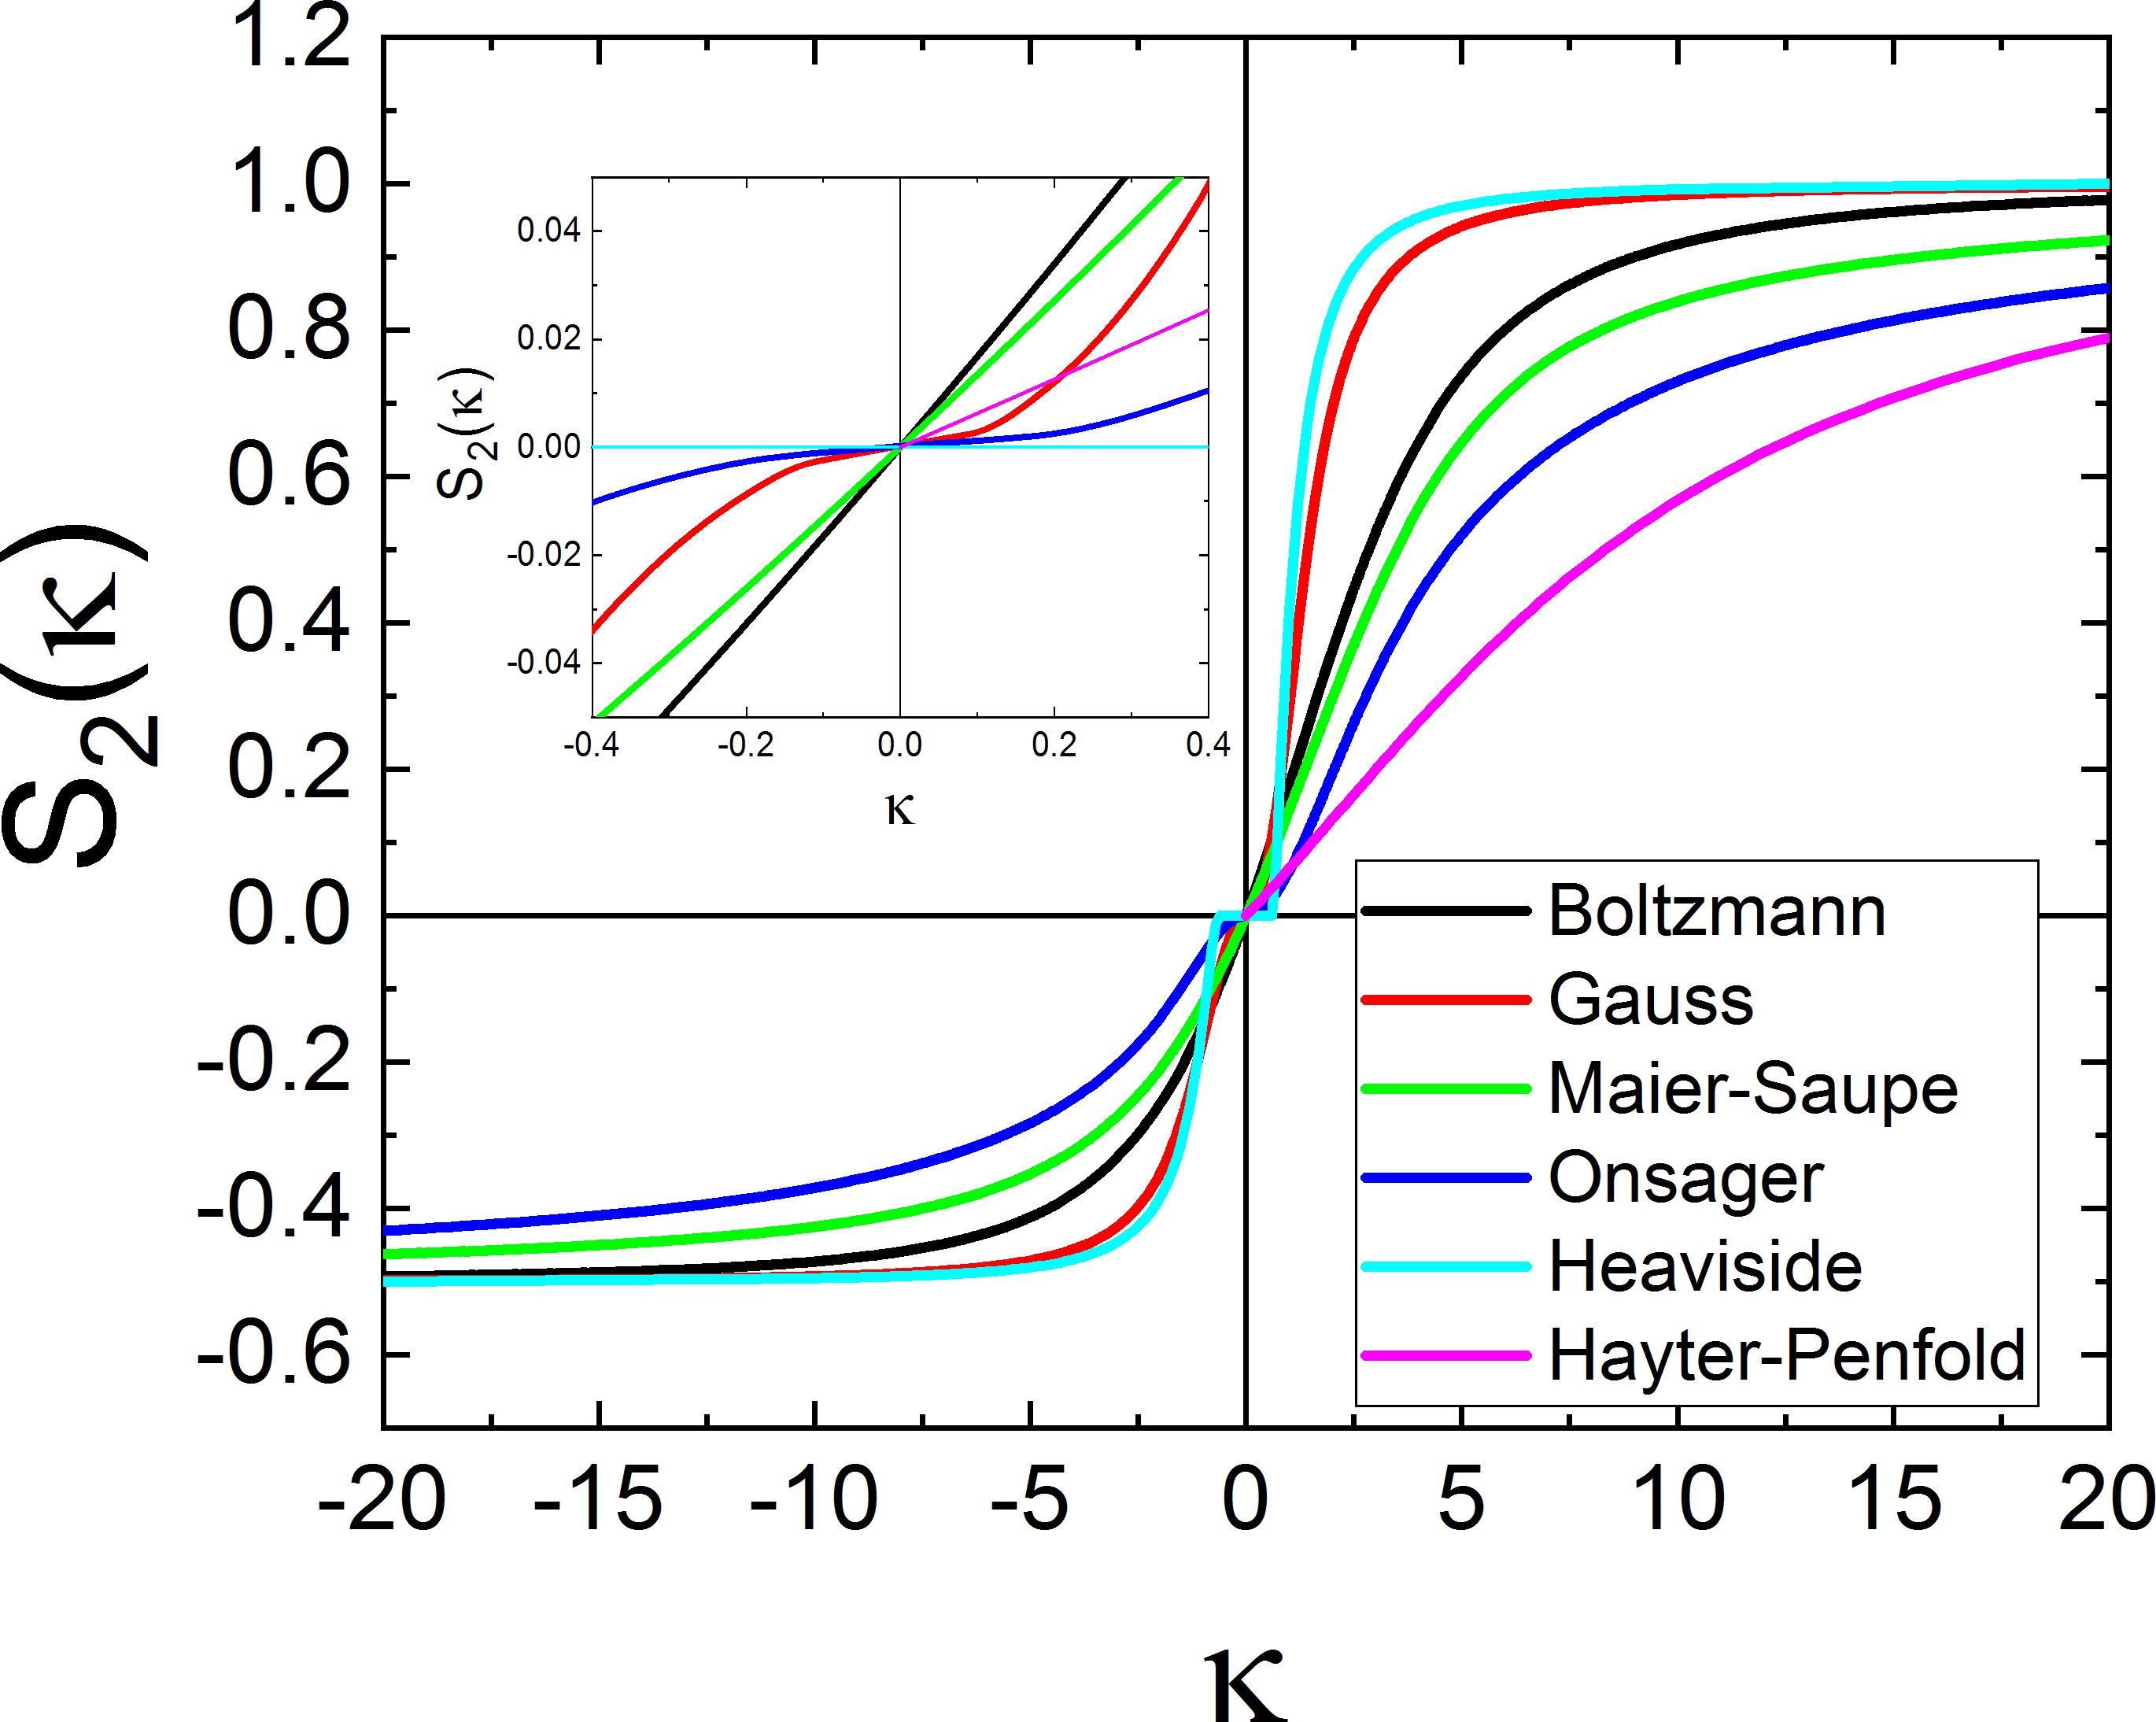
\includegraphics[width=0.75\textwidth]{../images/form_factor/cylindrical_obj/S2(kappa).png}
\end{center}
\caption{Order parameter $S_2(\kappa)$ for the orientation distributions described in the next subsections.}
\label{fig:S2_kappa}
\end{figure}

\begin{table}[htb]
\centering
\caption{Values for $\kappa$ to obtain certain order parameters $S_2(\kappa)$ for the different orientation distributions $p(\theta,\phi,\kappa)$.}
\label{tab:kappas}
\begin{tabular}{|l|llllllllll|}
\toprule
\diagbox{$p(\theta,\phi,\kappa)$}{$S_2(\kappa)$}  & -0.45    & -0.4    & -0.2    & 0 & 0.2    & 0.4    & 0.6    & 0.8    & 0.9    & 0.95    \\ \midrule
Gauss       & -3.739 & -1.62  & -1.128 & 0 & 0.83  & 1.220 & 1.686 & 2.576 & 3.762 & 5.4    \\
Boltzmann   & -7.141 & -4.59  & -1.431 & 0 & 1.114 & 2.218 & 3.581 & 5.989 & 9     & 13.08 \\
Maier-Saupe & -15    & -7.49  & -1.874 & 0 & 1.367 & 2.709 & 4.444 & 8.241 & 15.59 & 30.54 \\
Onsager     & -28.43 & -13.35 & -2.918 & 0 & 2.042 & 3.629 & 6.313 & 13.92 & 28.96 & 58.99 \\
Heavyside   & -3.108 & -2.157 &	-1.129 & 0 & 0.794 & 0.982 & 1.267 & 1.868 & 2.692 & 3.840 \\
Hayter-Penfold   & $\varnothing$ & $\varnothing$&	$\varnothing$ & 0 & 3.008 & 6.269 & 10.93 & 20.8 & 34.91 & 55.64  \\ \bottomrule
\end{tabular}
\end{table}

The order parameters $S_2$ can be calculated by
\begin{align}
S_2(\kappa) &=
\int_0^\pi \int_0^{2\pi}
                p(\theta,\phi;\kappa) \frac12 \left(3\cos^2\theta - 1\right) \sin \theta \, \mathrm{d}\theta\, \mathrm{d}\phi \nonumber \\
&= \int_0^\pi 2\pi
                p(\theta;\kappa) \frac12 \left(3\cos^2\theta - 1\right) \sin \theta \, \mathrm{d}\theta
\label{eq:S2kappa}
\end{align}
\begin{figure}[htb]
\captionsetup[subfigure]{position=b}
\centering
\subcaptionbox{Onsager orientation distribution for $\kappa=3$.  \label{fig:pOnsager3D1} }{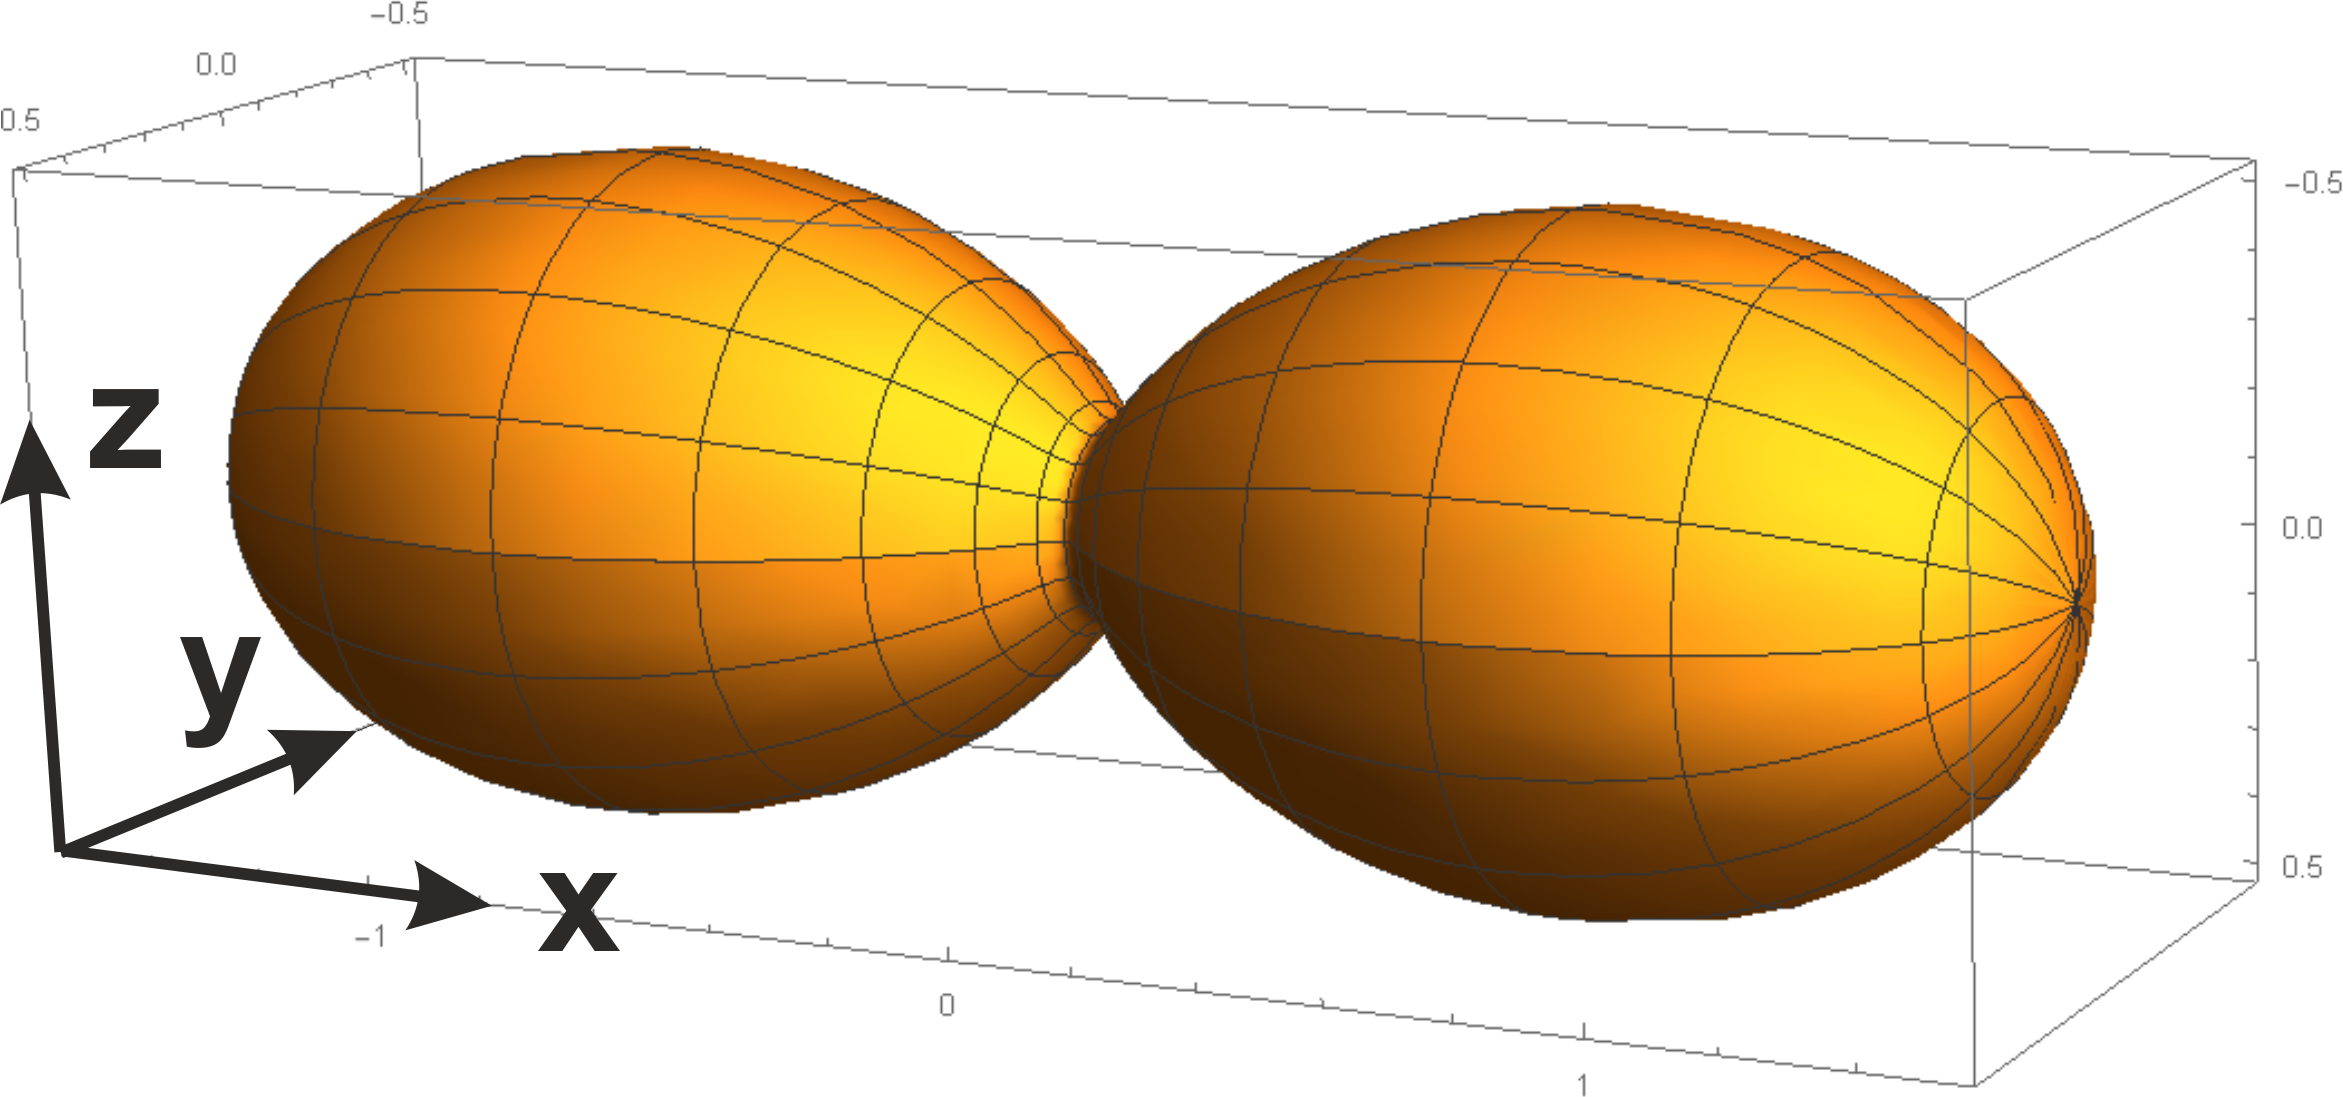
\includegraphics[width=0.55\textwidth]{../images/form_factor/cylindrical_obj/pOnsager(3).png}}
\hfill
\subcaptionbox{Onsager orientation distribution for $\kappa=-3$. \label{fig:pOnsager3D2}}{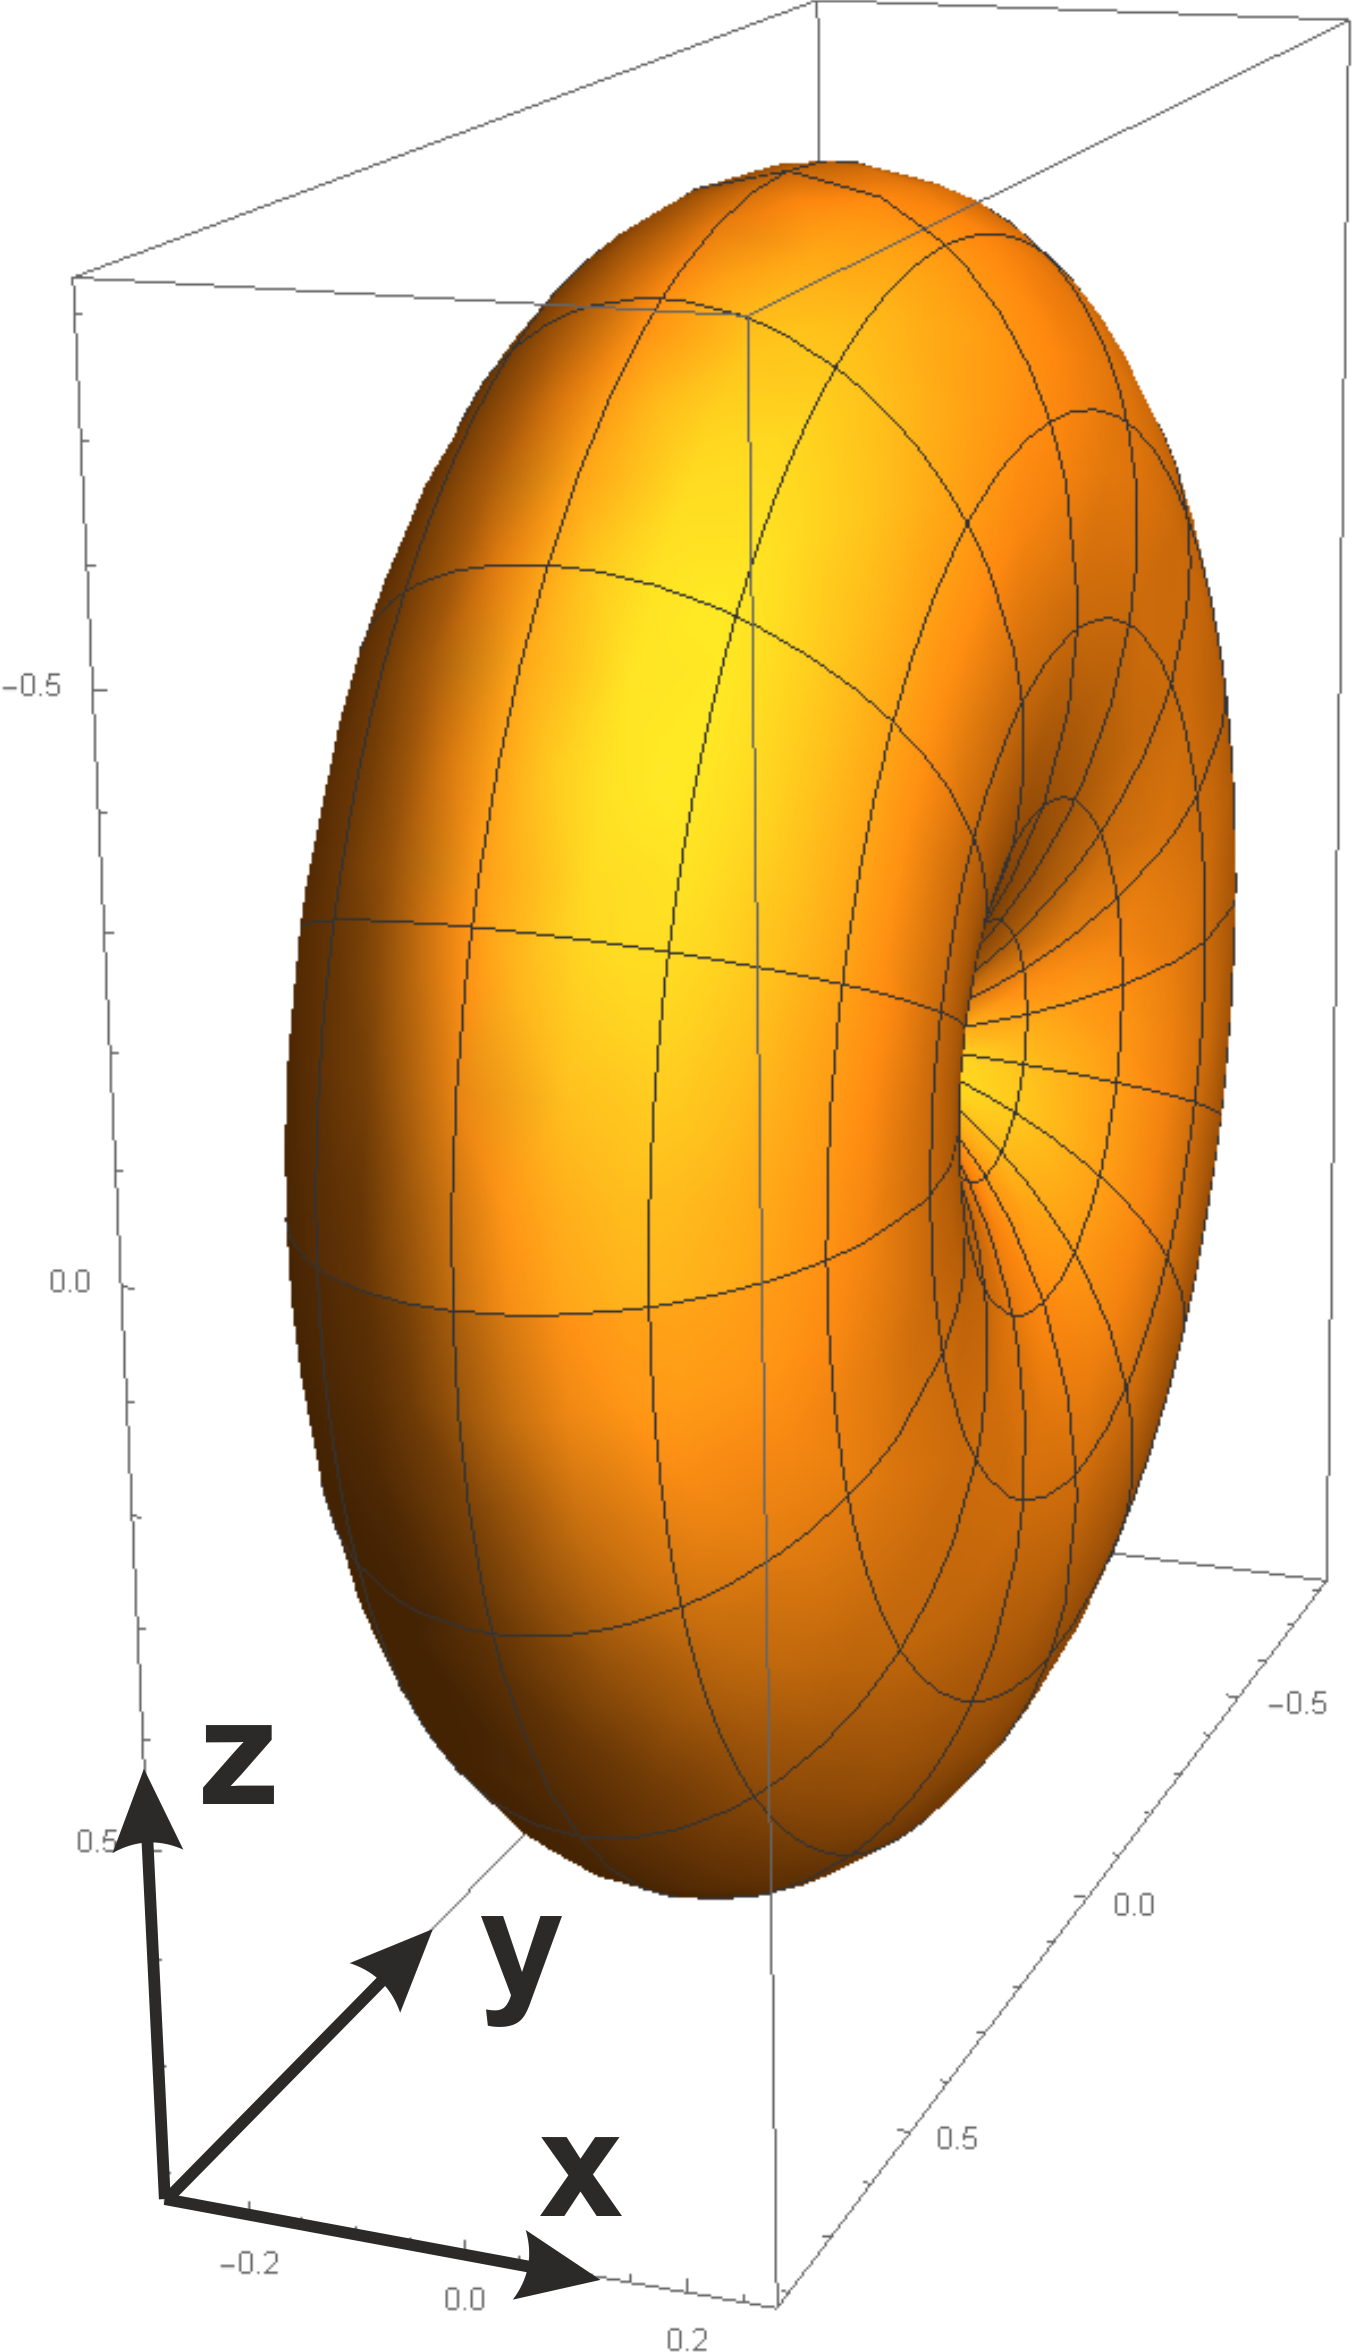
\includegraphics[width=0.4\textwidth]{../images/form_factor/cylindrical_obj/pOnsager(-3).png}}
\caption{Orientation distributions are are all independent on $\phi$ and have for $\kappa>0$ a positive order parameter, i.e. the most probable orientation is in the $\mathbf{x}$-direction and for $\kappa<0$ a negative order parameter, i.e. the most probable orientation lies in the $\mathbf{zy}$-plane}
\label{fig:pOnsager3D}
\end{figure}

\begin{figure}[htb]
\begin{center}
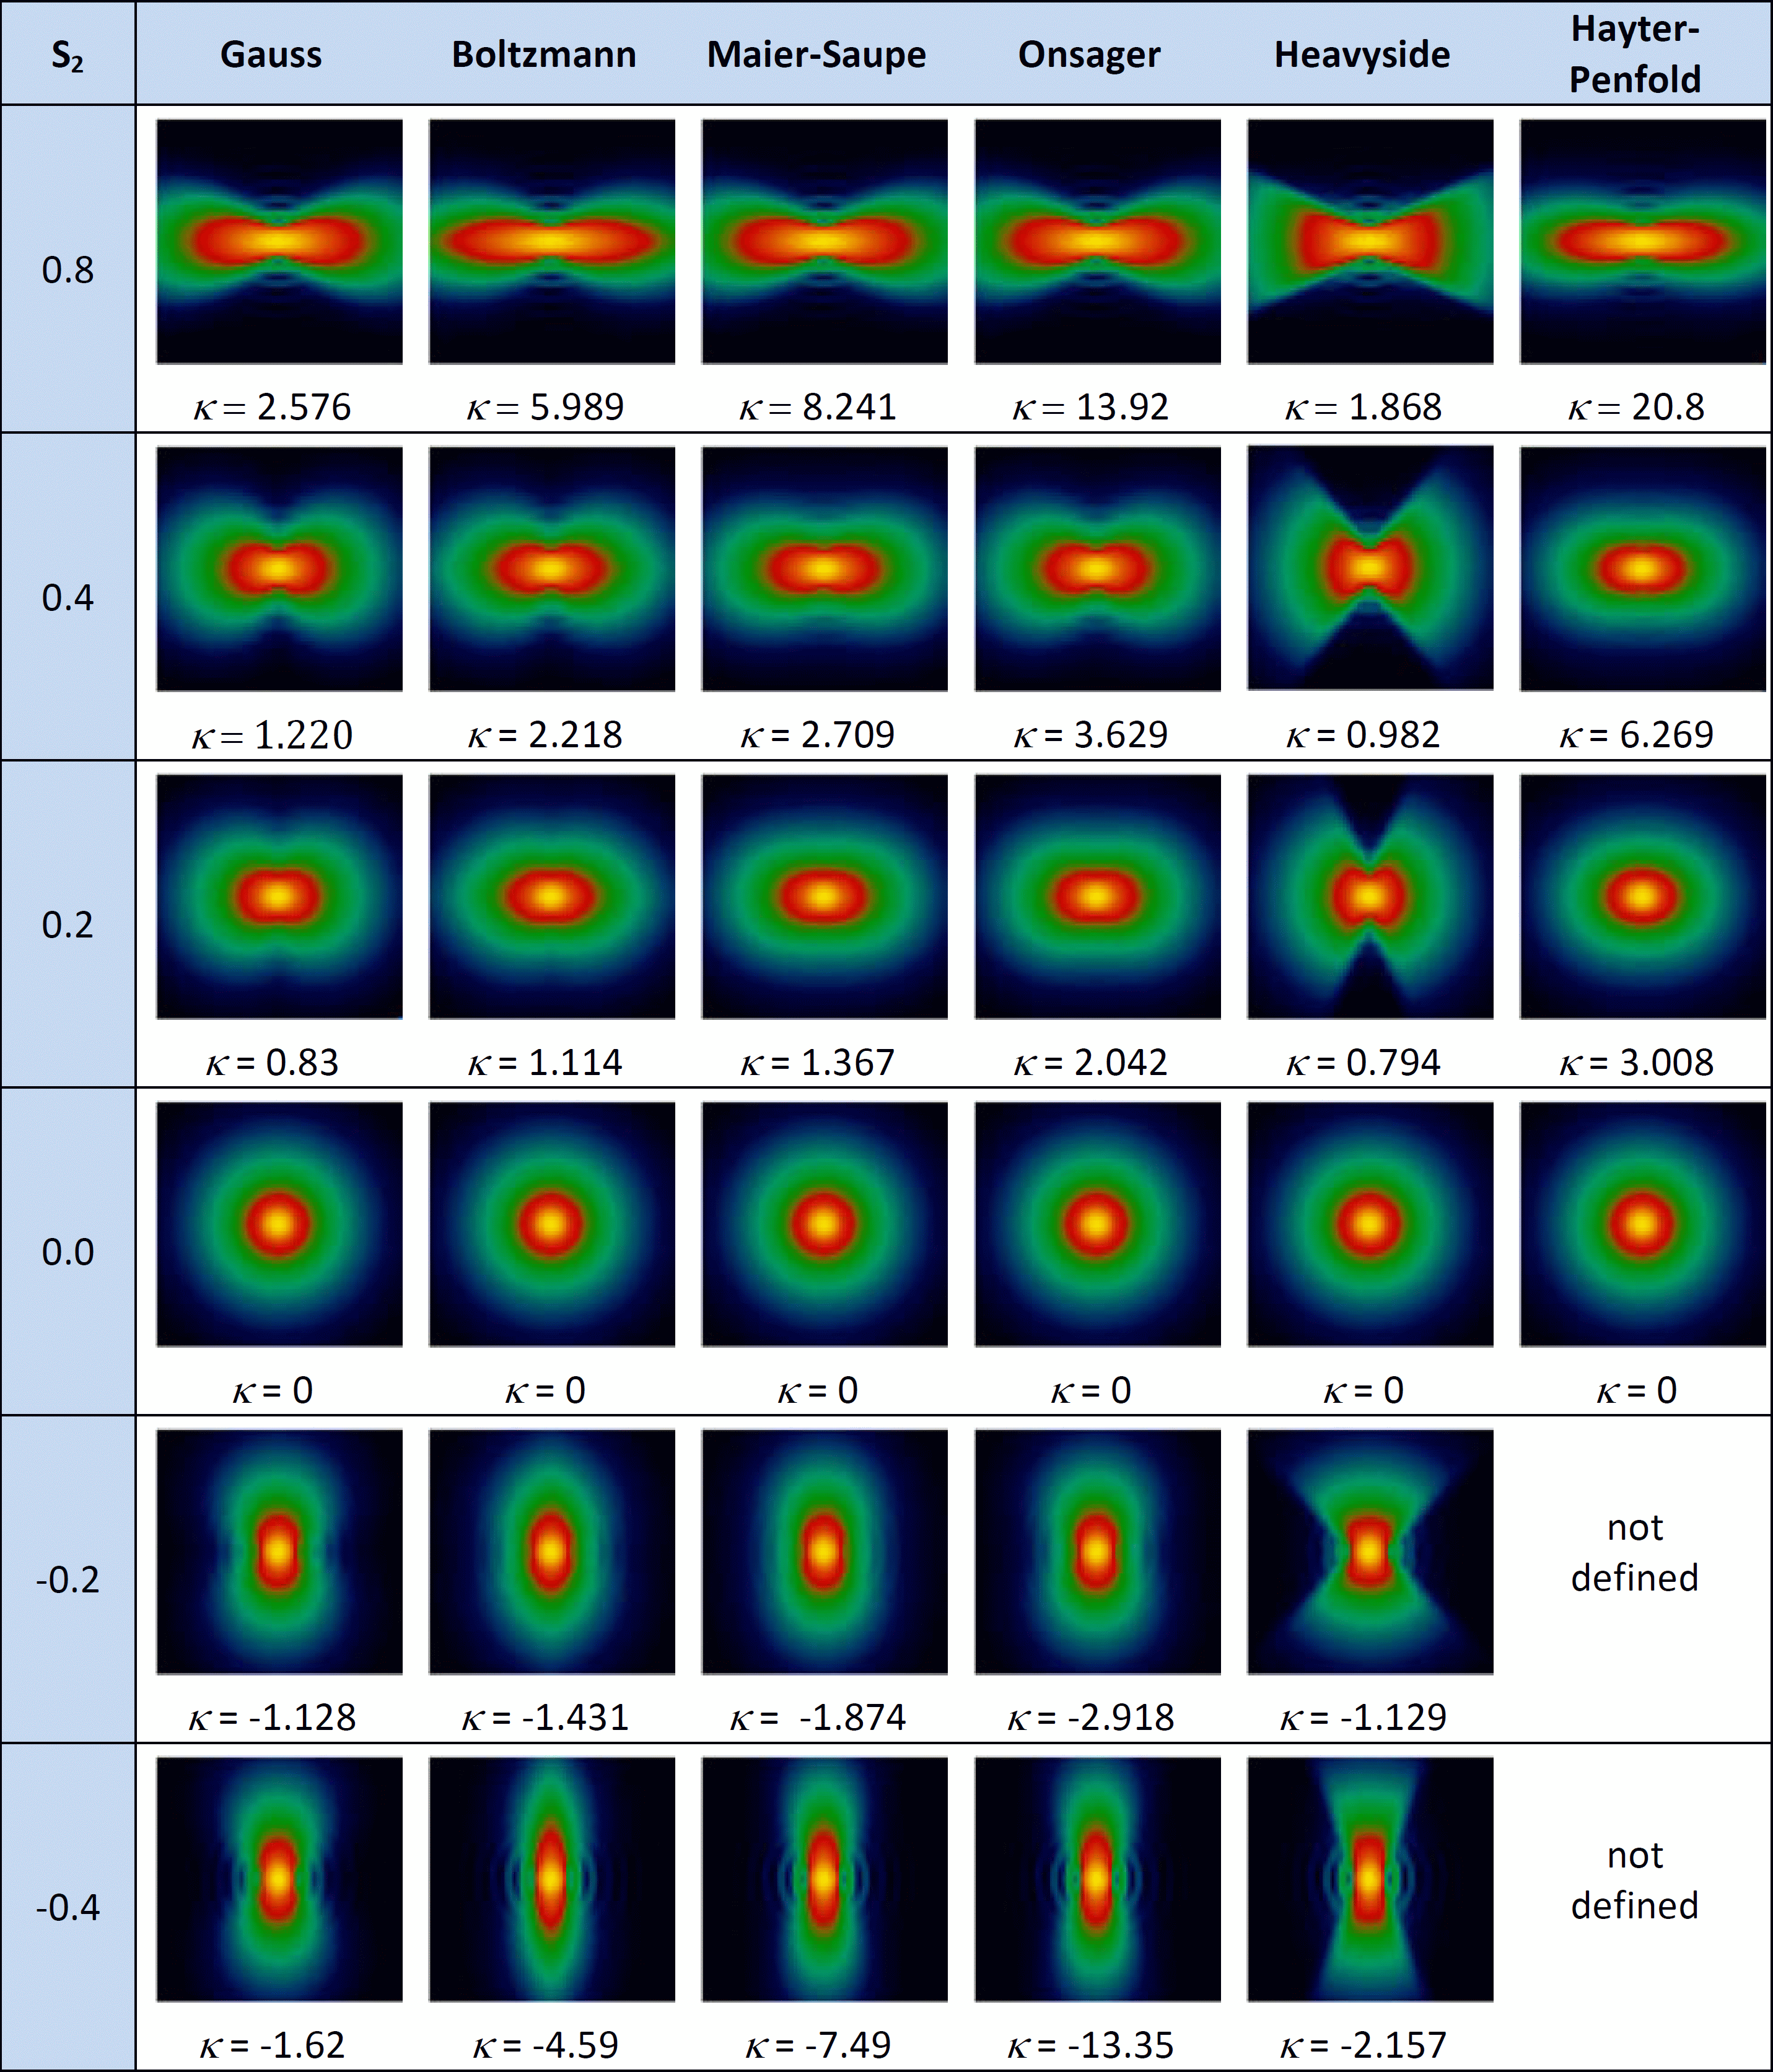
\includegraphics[width=0.95\textwidth]{../images/form_factor/cylindrical_obj/pXXXcomparison.png}
\end{center}
\caption{comparison of different orientation distributions with the same order parameter.}
\label{fig:S2_comparision}
\end{figure}

The order parameter for the Hayter-Penfold orientation distribution has been calculated by performing first a coordination transformation of the polar coordinates with $\mathbf{z}$ being the polar axis to coordination system with a polar axis pointing into the direction of the most probable orientation. The order parameter $S_2(\kappa)$ in eq.\ \ref{eq:S2kappa} is then calculated in this new polar coordinate system.

The form factors additional contain already a size distribution to profit from the speed enhancement by using a specialized multidimensional integration routine. The size distribution is included as
\begin{align}
I(Q) &= \int_0^\infty \mathrm{LogNorm}(\nu,\sigma,1) I_\mathrm{p.a.CylShell}(Q,R\nu,\Delta R\nu,L\nu) \, \mathrm{d}\nu \\
\end{align}
and
\begin{align}
I(Q) &= \int_0^\infty \mathrm{LogNorm}(\nu,\sigma,1) I_\mathrm{p.a.EllShell}(Q,R_\mathrm{p}\nu,\Delta R\nu,R_\mathrm{e}\nu) \, \mathrm{d}\nu
\end{align}
 with
\begin{align}
\mathrm{LogNorm}(\nu,\sigma,\mu) &= \frac{1}{\sqrt{2\pi}\sigma}\frac{1}{\nu} \exp\left(-\frac{(\ln(\nu/\mu))^2}{2\sigma^2}\right)
\end{align}

%%%%%%%%%%%%%%%%%%%%%%%%%%%%%%%%%%%%%%%%%%%%%%%%%%%%%%%%%%%%%%%%%%%%%%%%%%%%%%%%%%%%%%%%%%%%%%%%%%%%%%%%%
\clearpage
\subsubsection{Maier-Saupe orientation distribution} ~\\

\begin{figure}[htb]
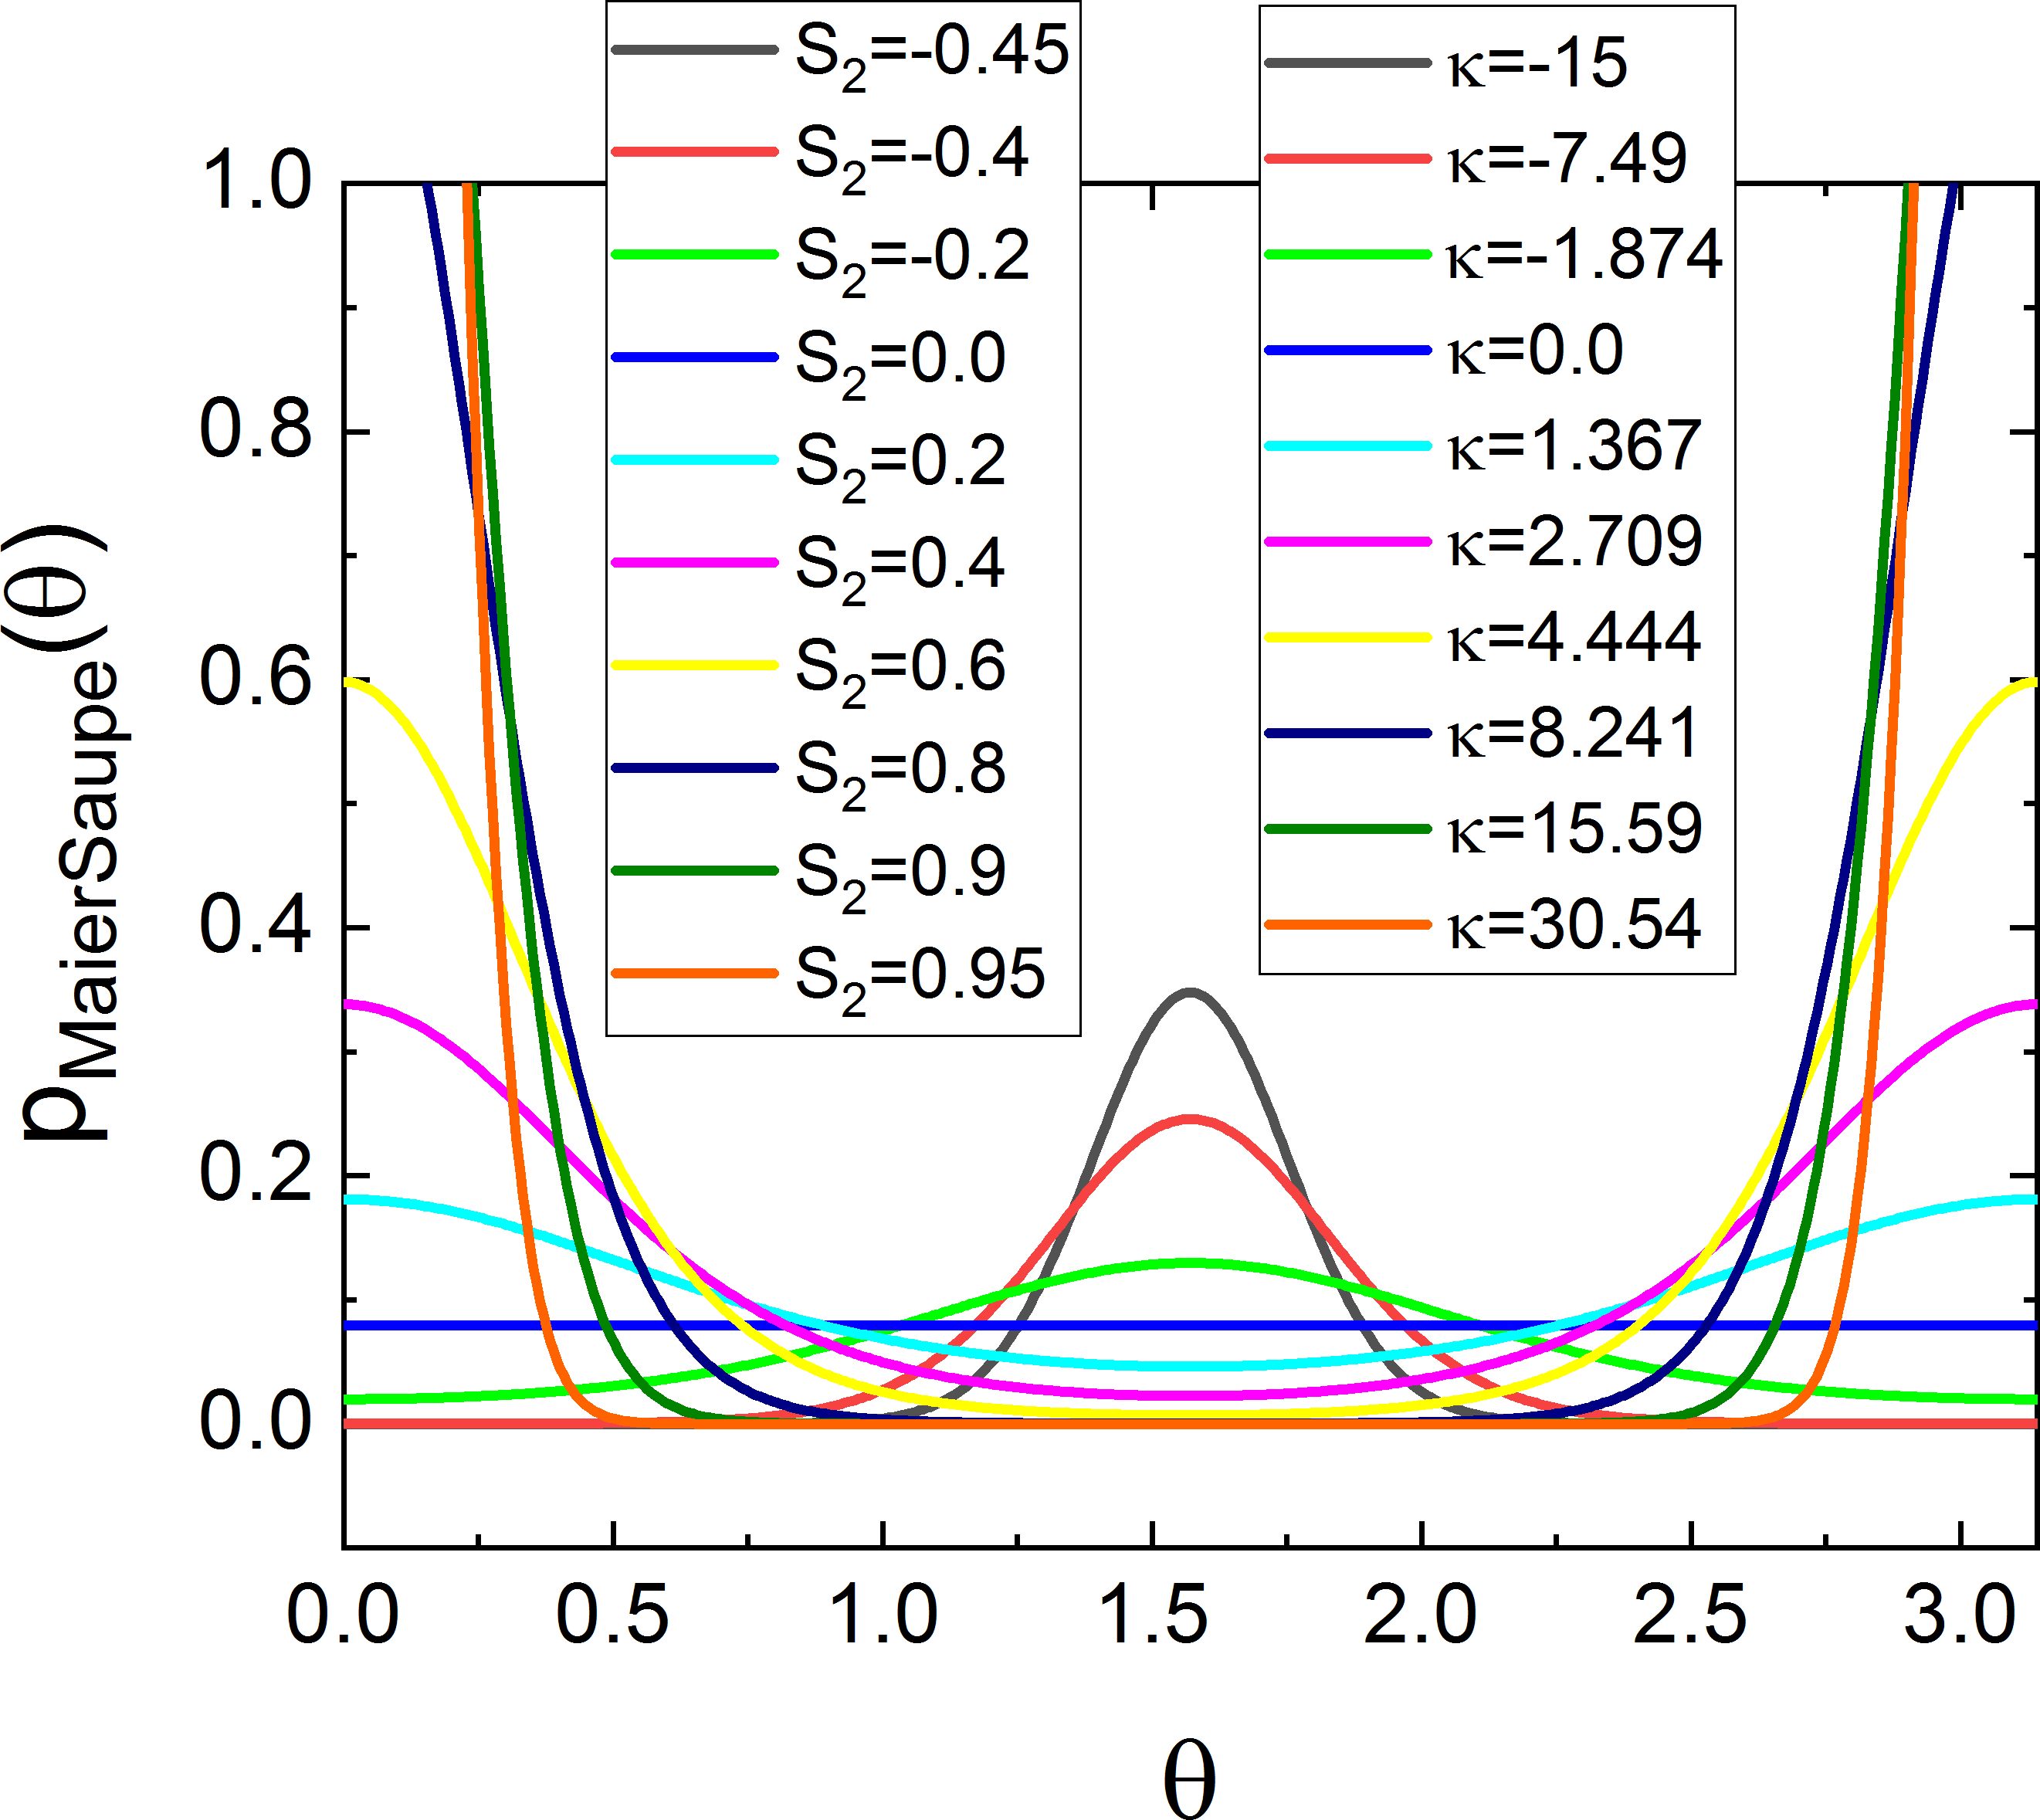
\includegraphics[width=0.75\textwidth]{../images/form_factor/cylindrical_obj/pMaierSaupeGr.png}
\caption{Maier-Saupe orientation distribution $p_\mathrm{MS}(\theta,\kappa)$ for different values of $\kappa$, resulting in an order parameter as listed in table \ref{tab:kappas}.}
\label{fig:pMaierSaupeGr}
\end{figure}

\begin{align}
p(\theta,\phi;\kappa) & = \frac{1}{c_\mathrm{MS}}\exp\left(\kappa \cos^2\theta\right)
\end{align}
with
\begin{align}
c_\mathrm{MS} &=
\begin{cases}
\displaystyle
4\pi\exp(\kappa) \frac{\mathrm{D}\left(\sqrt{\kappa}\right)}{\sqrt{\kappa}}   &\mathrm{for~} \kappa > 0 \\[5mm]
\displaystyle
2\pi \sqrt{\pi} \frac{\mathrm{erf}\left(\sqrt{\abs{\kappa}}\right)}{\sqrt{\abs{\kappa}}}  &\mathrm{for~} \kappa < 0 \\[2mm]
\displaystyle
4\pi                                                                                      &\mathrm{for~} \kappa = 0
\end{cases}
\end{align}
with $D(x)$ being Dawson's integral $D(x)=e^{-x^2}\int_0^x e^{y^2} \mathrm{d}y = \frac12\sqrt{\pi}e^{-x^2}\mathrm{erfi}(x)$

\vspace{5mm}

\underline{Input Parameters for model \texttt{Sheared Cylinders (Maier-Saupe)}:}\\
\begin{description}
\item[\texttt{R}] radius of cylinders $R$
\item[\texttt{t}] shell thickness $t$
\item[\texttt{L}] cylinder length $L$
\item[\texttt{eta\_core}] scattering length density of cylinder core $\eta_\mathrm{core}$
\item[\texttt{eta\_shell}] scattering length density of cylinder shell $\eta_\mathrm{shell}$
\item[\texttt{eta\_solv}] scattering length density of solvent $\eta_\mathrm{solv}$
\item[\texttt{psi}] direction of scattering vector on the detector $\psi$
\item[{\texttt{sigma}}] width parameter of lognormal size distribution $\sigma$
\item[{\texttt{kappa}}] orientation distribution parameter $\kappa$
\end{description}

\vspace{5mm}

\underline{Input Parameters for model \texttt{Sheared Spheroids (Maier-Saupe)}:}\\
\begin{description}
\item[\texttt{R\_equatorial}] equatorial semi-axes of spheroids $R_\mathrm{e}$
\item[\texttt{t}] shell thickness $t$
\item[\texttt{R\_polar}] polar semi-axis of spheroids $R_\mathrm{p}$
\item[\texttt{eta\_core}] scattering length density of cylinder core $\eta_\mathrm{core}$
\item[\texttt{eta\_shell}] scattering length density of cylinder shell $\eta_\mathrm{shell}$
\item[\texttt{eta\_solv}] scattering length density of solvent $\eta_\mathrm{solv}$
\item[\texttt{psi}] direction of scattering vector on the detector $\psi$
\item[{\texttt{sigma}}] width parameter of lognormal size distribution $\sigma$
\item[{\texttt{kappa}}] orientation distribution parameter $\kappa$
\end{description}

\vspace{5mm}

\underline{Note:}
\begin{itemize}
\item The size distribution is taken simultaneously over all parameters $R$, $t$, $L$, and $R_\mathrm{e}$, $t$, $R_\mathrm{p}$ respectively, so that their aspect ratios always stay constant.
\end{itemize}
%%%%%%%%%%%%%%%%%%%%%%%%%%%%%%%%%%%%%%%%%%%%%%%%%%%%%%%%%%%%%%%%%%%%%%%%%%%%%%%%%%

\newpage
\subsubsection{Onsager orientation distribution} ~\\

\begin{figure}[htb]
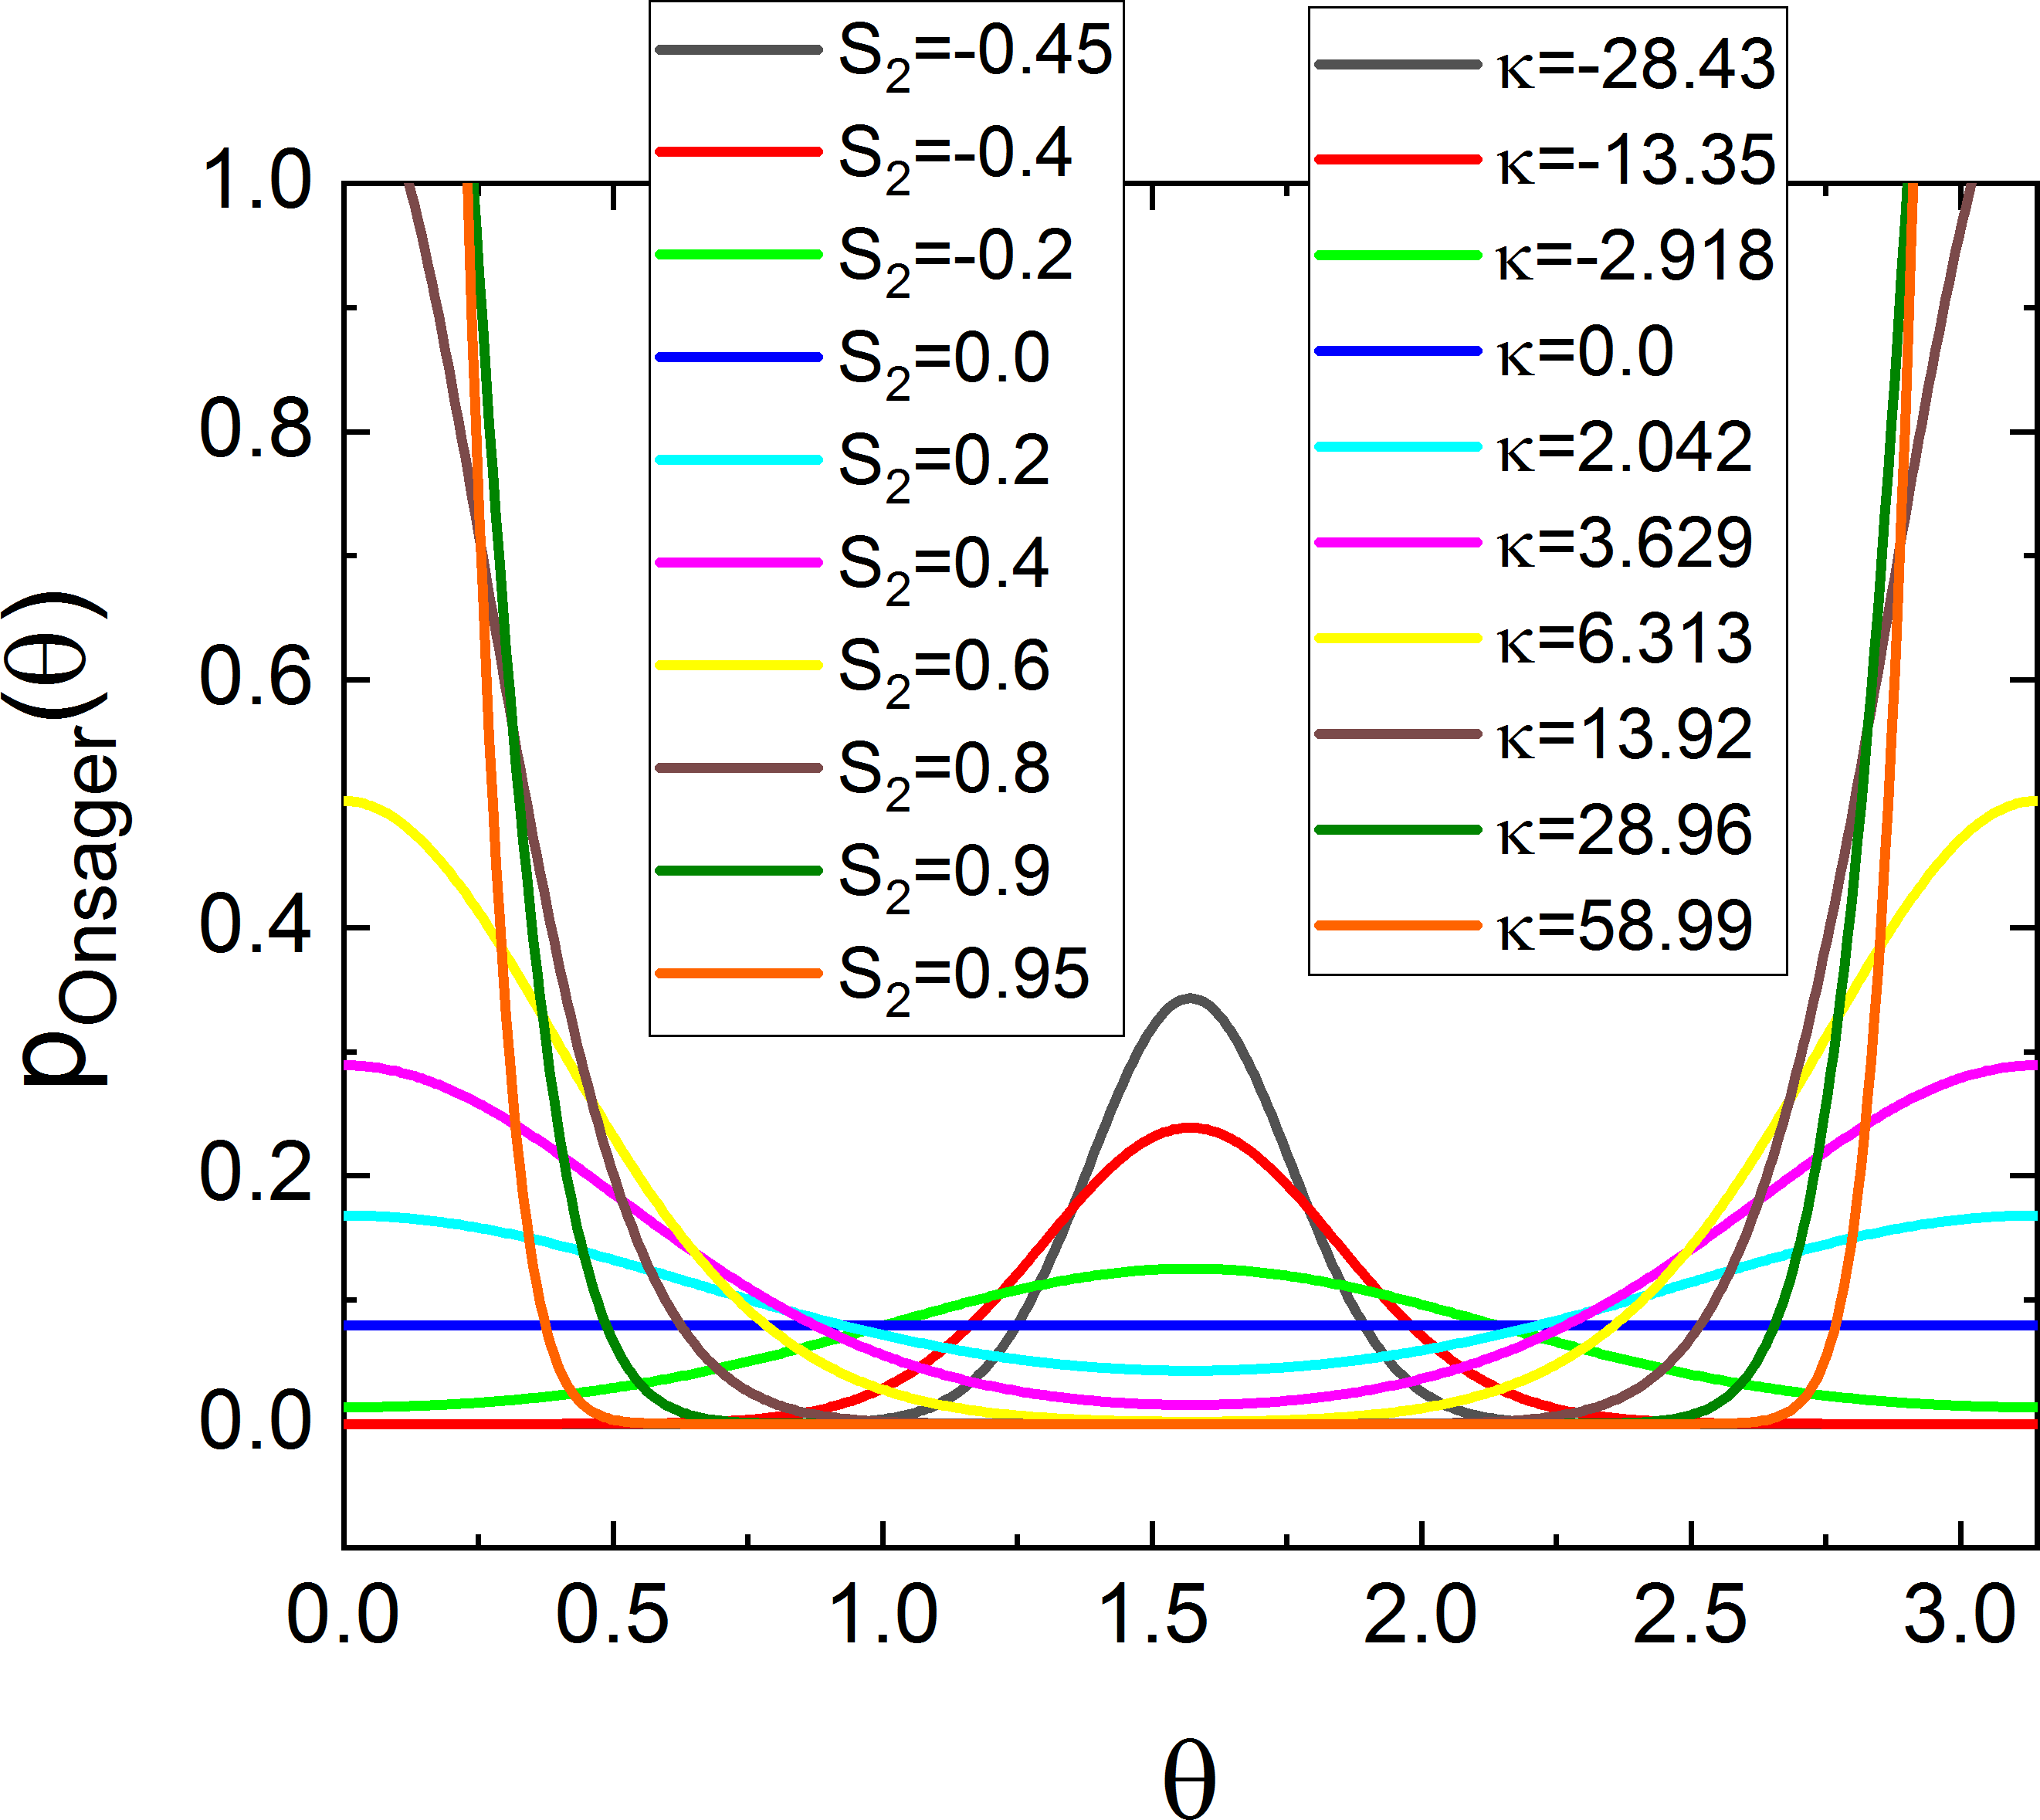
\includegraphics[width=0.75\textwidth]{../images/form_factor/cylindrical_obj/pOnsagerGr.png}
\caption{Onsager orientation distribution $p_\mathrm{O}(\theta,\kappa)$ for different values of $\kappa$, resulting in an order parameter as listed in table \ref{tab:kappas}.}
\label{fig:pOnsagerGr}
\end{figure}

\begin{align}
p_\mathrm{O}(\theta,\phi;\kappa) & =
\begin{cases} \displaystyle
\frac{\kappa \cosh\left(\kappa \cos(\theta)\right)}{4\pi \sinh(\kappa)}      &\mathrm{for~} \kappa \geq 0 \\[5mm]
 \displaystyle
\frac{\cosh\left(\abs{\kappa} \sin(\theta)\right)}{2\pi^2 L_1(\abs{\kappa})}  &\mathrm{for~} \kappa < 0
\end{cases}
\end{align}
where $L_\nu(x)$ is the modified Struve function.

\vspace{5mm}

\underline{Input Parameters for model \texttt{Sheared Cylinders (Onsager)}:}\\
\begin{description}
\item[\texttt{R}] radius of cylinders $R$
\item[\texttt{t}] shell thickness $t$
\item[\texttt{L}] cylinder length $L$
\item[\texttt{eta\_core}] scattering length density of cylinder core $\eta_\mathrm{core}$
\item[\texttt{eta\_shell}] scattering length density of cylinder shell $\eta_\mathrm{shell}$
\item[\texttt{eta\_solv}] scattering length density of solvent $\eta_\mathrm{solv}$
\item[\texttt{psi}] direction of scattering vector on the detector $\psi$
\item[{\texttt{sigma}}] width parameter of lognormal size distribution $\sigma$
\item[{\texttt{kappa}}] orientation distribution parameter $\kappa$
\end{description}

\vspace{5mm}

\underline{Input Parameters for model \texttt{Sheared Spheroids (Onsager}:}\\
\begin{description}
\item[\texttt{R\_equatorial}] equatorial semi-axes of spheroids $R_\mathrm{e}$
\item[\texttt{t}] shell thickness $t$
\item[\texttt{R\_polar}] polar semi-axis of spheroids $R_\mathrm{p}$
\item[\texttt{eta\_core}] scattering length density of cylinder core $\eta_\mathrm{core}$
\item[\texttt{eta\_shell}] scattering length density of cylinder shell $\eta_\mathrm{shell}$
\item[\texttt{eta\_solv}] scattering length density of solvent $\eta_\mathrm{solv}$
\item[\texttt{psi}] direction of scattering vector on the detector $\psi$
\item[{\texttt{sigma}}] width parameter of lognormal size distribution $\sigma$
\item[{\texttt{kappa}}] orientation distribution parameter $\kappa$
\end{description}

\vspace{5mm}

\underline{Note:}
\begin{itemize}
\item The size distribution is taken simultaneously over all parameters $R$, $t$, $L$, and $R_\mathrm{e}$, $t$, $R_\mathrm{p}$ respectively, so that their aspect ratios always stay constant.
\end{itemize}
%%%%%%%%%%%%%%%%%%%%%%%%%%%%%%%%%%%%%%%%%%%%%%%%%%%%%%%%%%%%%%%%%%%%%%%%%%%%%%%%%%

\newpage
\subsubsection{Boltzmann orientation distribution} ~\\

\begin{figure}[htb]
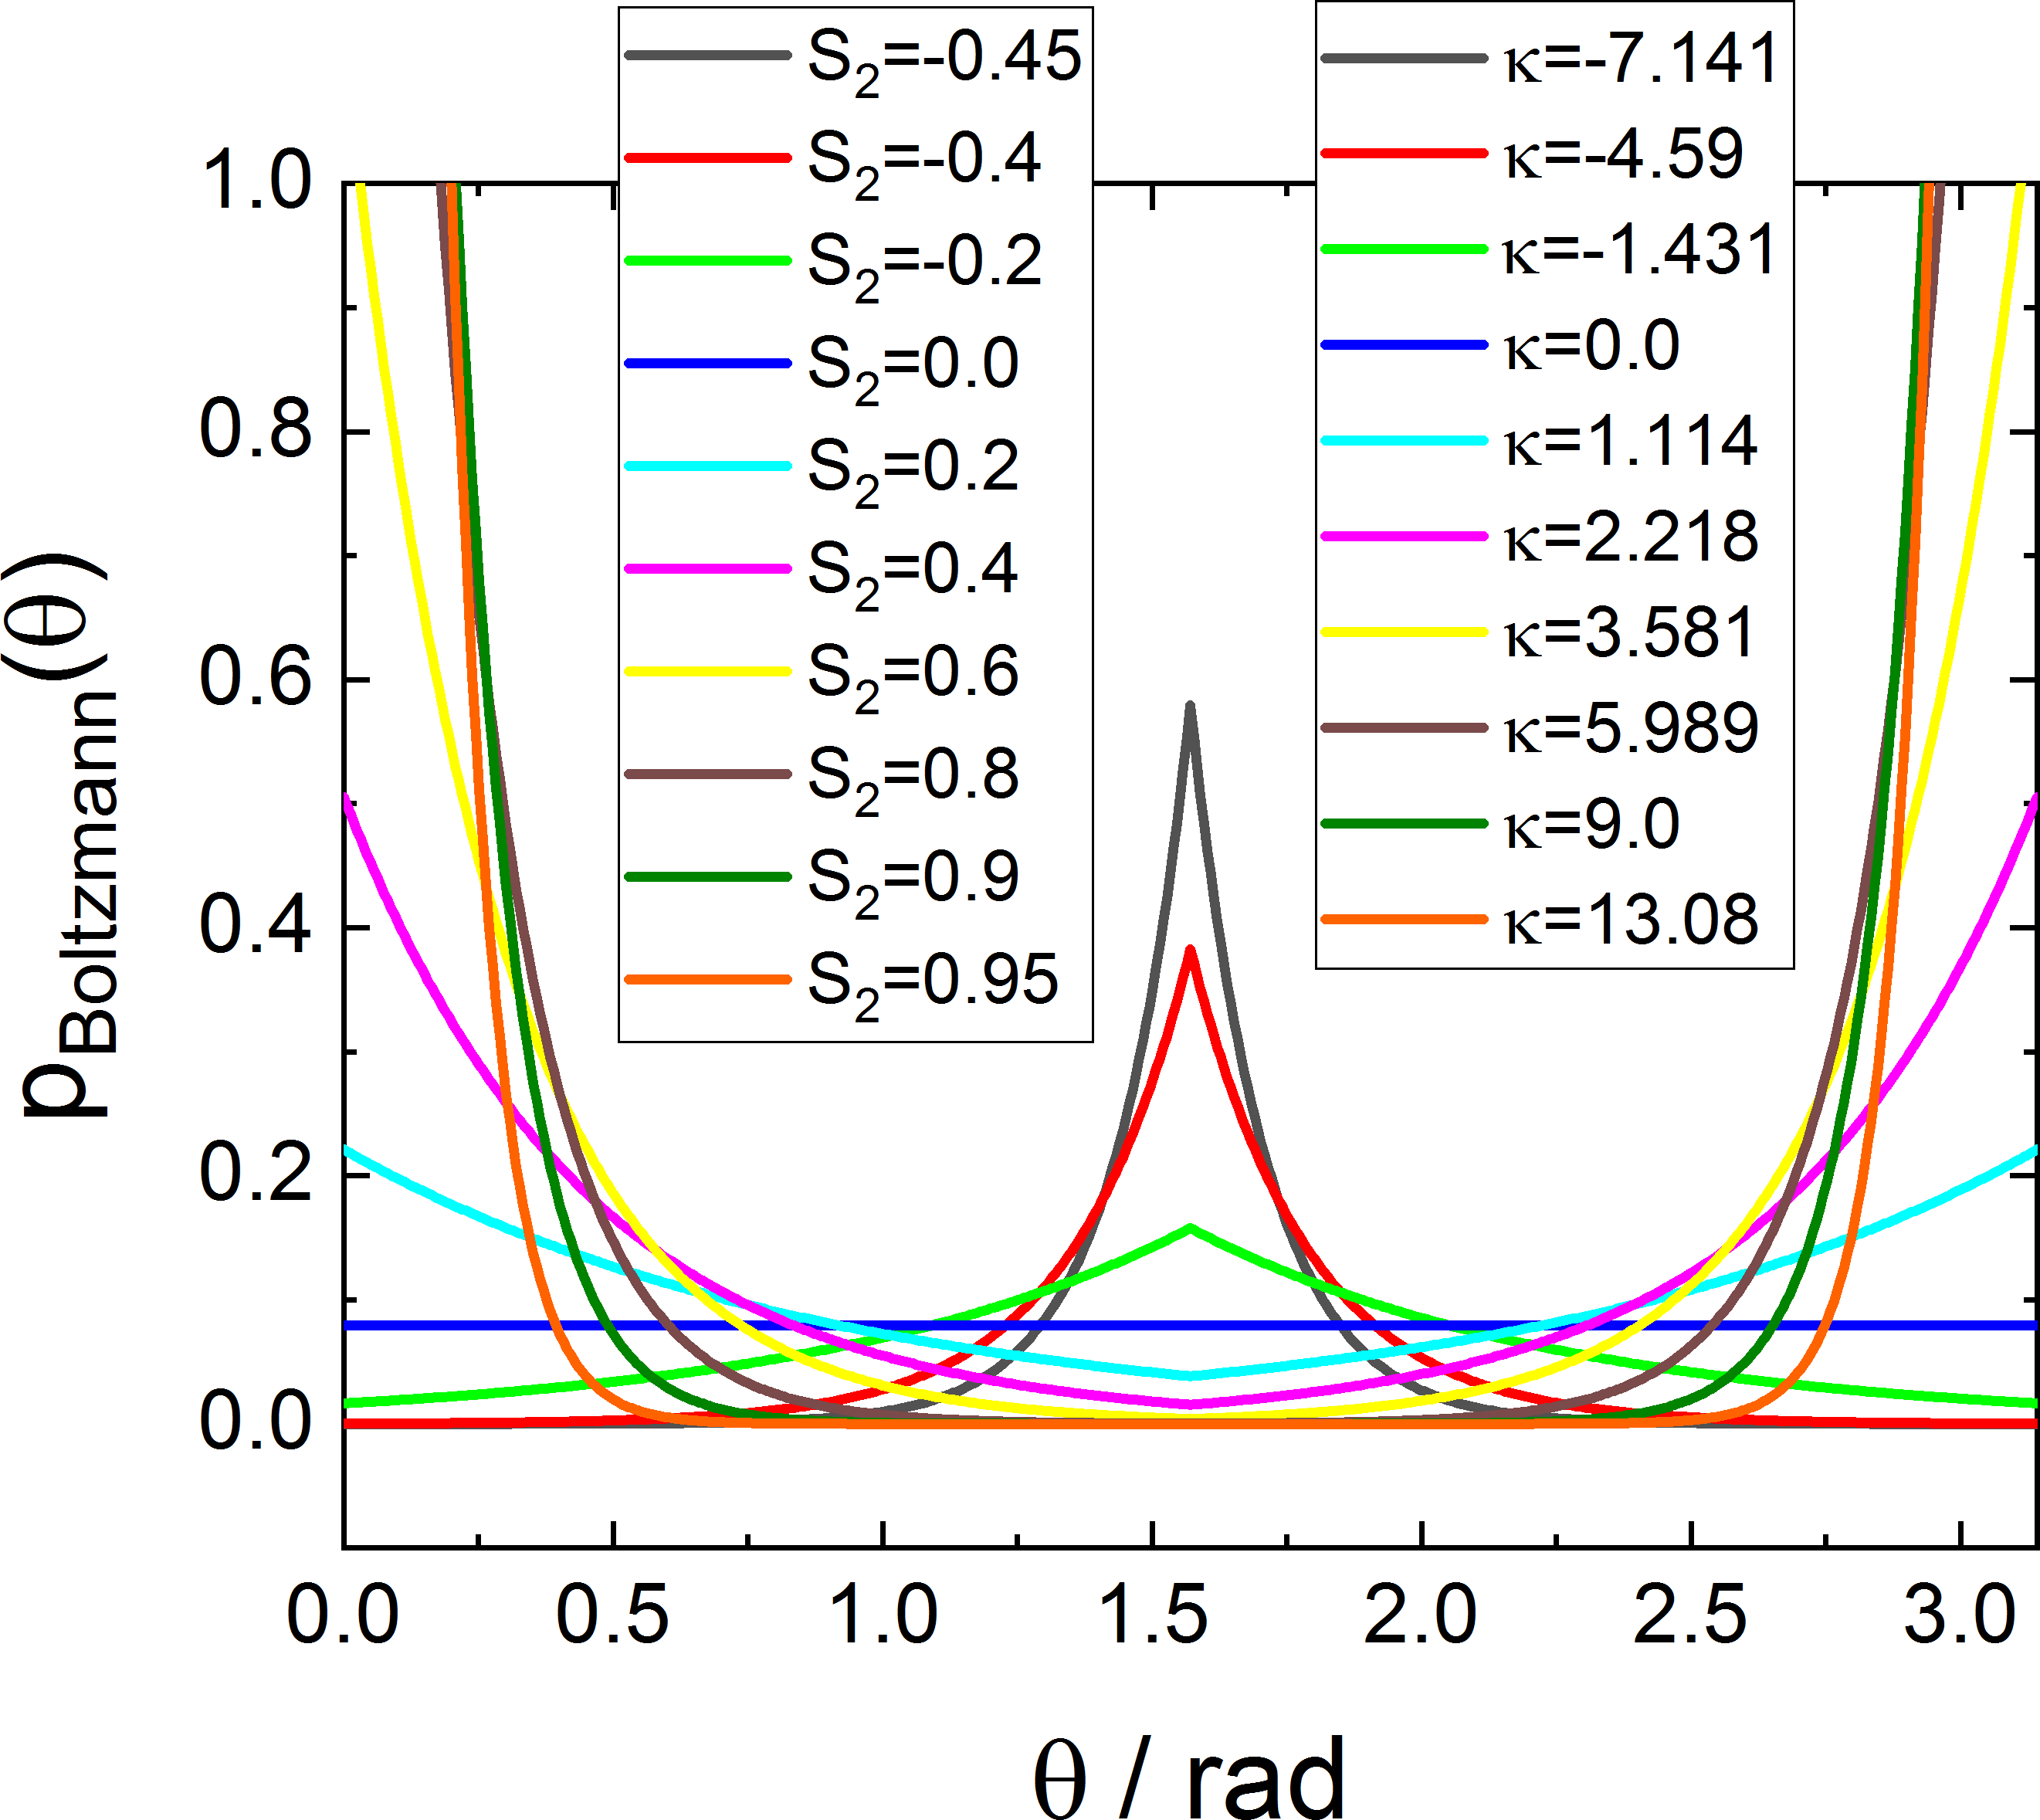
\includegraphics[width=0.75\textwidth]{../images/form_factor/cylindrical_obj/pBoltzmannGr.png}
\caption{Boltzmann orientation distribution $p_\mathrm{B}(\theta,\kappa)$ for different values of $\kappa$, resulting in an order parameter as listed in table \ref{tab:kappas}.}
\label{fig:pBoltzmannGr}
\end{figure}

\begin{align}
p_\mathrm{B}(\theta,\phi;\kappa) & =
\begin{cases}
\displaystyle
\frac{1}{2\pi c_\mathrm{B}}\exp\left(-\theta\kappa\right) & \mathrm{for~}  \theta \leq \frac{\pi}{2}\\[5mm]
\displaystyle
\frac{1}{2\pi c_\mathrm{B}}\exp\left(-(\pi-\theta)\kappa\right) & \mathrm{for~}  \theta > \frac{\pi}{2}
\end{cases}
\end{align}
with
\begin{align}
c_\mathrm{B} &= \frac{2\left(1-\kappa \exp\left(-\frac{\pi}{2}\kappa\right)\right)}{\kappa^2+1}
\end{align}

\vspace{5mm}

\underline{Input Parameters for model \texttt{Sheared Cylinders (Boltzmann)}:}\\
\begin{description}
\item[\texttt{R}] radius of cylinders $R$
\item[\texttt{t}] shell thickness $t$
\item[\texttt{L}] cylinder length $L$
\item[\texttt{eta\_core}] scattering length density of cylinder core $\eta_\mathrm{core}$
\item[\texttt{eta\_shell}] scattering length density of cylinder shell $\eta_\mathrm{shell}$
\item[\texttt{eta\_solv}] scattering length density of solvent $\eta_\mathrm{solv}$
\item[\texttt{psi}] direction of scattering vector on the detector $\psi$
\item[{\texttt{sigma}}] width parameter of lognormal size distribution $\sigma$
\item[{\texttt{kappa}}] orientation distribution parameter $\kappa$
\end{description}

\vspace{5mm}

\underline{Input Parameters for model \texttt{Sheared Spheroids (Boltzmann)}:}\\
\begin{description}
\item[\texttt{R\_equatorial}] equatorial semi-axes of spheroids $R_\mathrm{e}$
\item[\texttt{t}] shell thickness $t$
\item[\texttt{R\_polar}] polar semi-axis of spheroids $R_\mathrm{p}$
\item[\texttt{eta\_core}] scattering length density of cylinder core $\eta_\mathrm{core}$
\item[\texttt{eta\_shell}] scattering length density of cylinder shell $\eta_\mathrm{shell}$
\item[\texttt{eta\_solv}] scattering length density of solvent $\eta_\mathrm{solv}$
\item[\texttt{psi}] direction of scattering vector on the detector $\psi$
\item[{\texttt{sigma}}] width parameter of lognormal size distribution $\sigma$
\item[{\texttt{kappa}}] orientation distribution parameter $\kappa$
\end{description}

\vspace{5mm}

\underline{Note:}
\begin{itemize}
\item The size distribution is taken simultaneously over all parameters $R$, $t$, $L$, and $R_\mathrm{e}$, $t$, $R_\mathrm{p}$ respectively, so that their aspect ratios always stay constant.
\end{itemize}
%%%%%%%%%%%%%%%%%%%%%%%%%%%%%%%%%%%%%%%%%%%%%%%%%%%%%%%%%%%%%%%%%%%%%%%%%%%%%%%%%%

\newpage
\subsubsection{Gaussian orientation distribution}
\label{sect:ShearedCylinderGaussian}
~\\

\begin{figure}[htb]
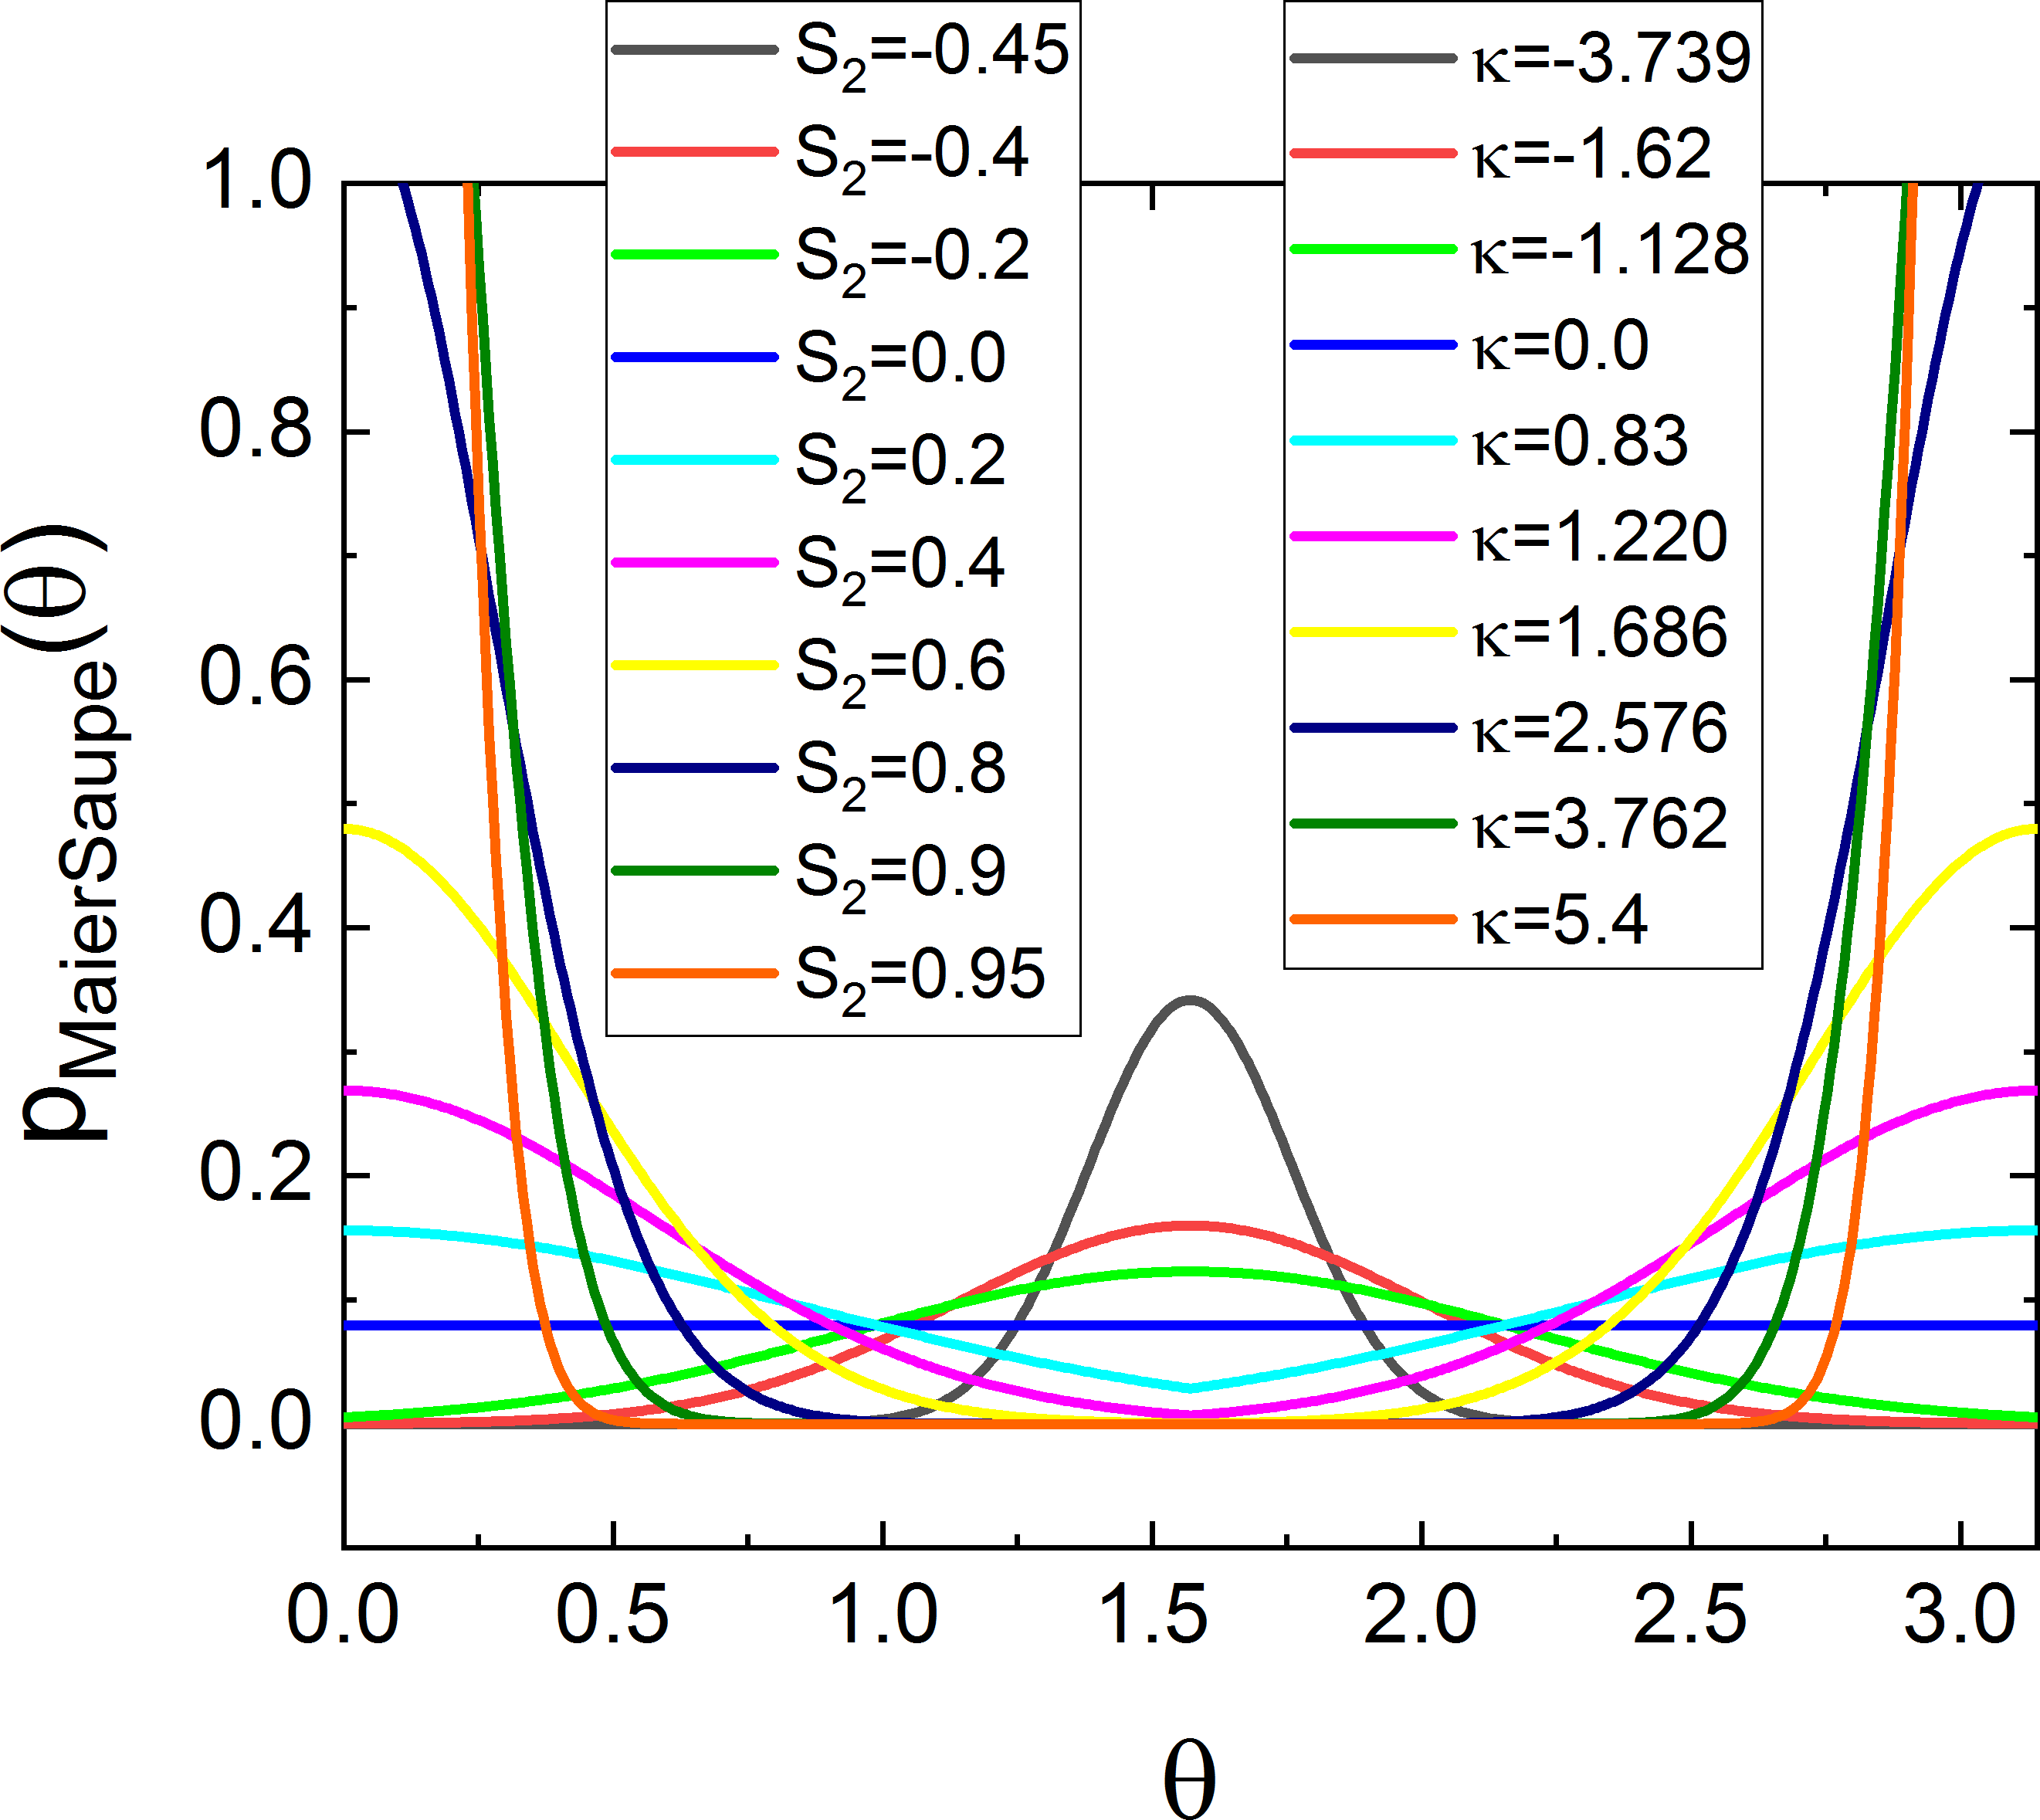
\includegraphics[width=0.75\textwidth]{../images/form_factor/cylindrical_obj/pGaussGr.png}
\caption{Gaussian orientation distribution $p_\mathrm{G}(\theta,\kappa)$ for different values of $\kappa$, resulting in an order parameter as listed in table \ref{tab:kappas}.}
\label{fig:pGaussGr}
\end{figure}

\begin{align}
p_\mathrm{G}(\theta,\phi;\kappa) & =
\begin{cases}
\displaystyle
\frac{1}{2\pi c_\mathrm{G}}\exp\left(-\theta^2\kappa^2\right) & \mathrm{for~} \kappa \geq 0 \mathrm{~and~} \theta \leq \frac{\pi}{2}\\[5mm]
\displaystyle
\frac{1}{2\pi c_\mathrm{G}}\exp\left(-\left(\pi-\theta\right)^2\kappa^2\right) & \mathrm{for~} \kappa \geq 0 \mathrm{~and~} \theta > \frac{\pi}{2}\\[5mm]
\displaystyle
\frac{1}{2\pi c_\mathrm{G}}\exp\left(-\left(\frac{\pi}{2}-\theta\right)^2\abs{\kappa}^2\right) & \mathrm{for~} \kappa < 0
\end{cases}
\end{align}
with
\begin{align}
c_\mathrm{G} & =
\begin{cases}\displaystyle
\frac{D\left(\kappa/2\right)}{\kappa}
           +\frac{\sqrt{\pi}}{2\kappa} e^{-\frac{1}{4\kappa^2}} \Re\left(\mathrm{cerfi}\left(-\frac{1}{2\kappa}+\imath\frac{\pi}{2}\kappa\right) \right)& \mathrm{for~} \kappa \geq 0 \\[5mm]
\displaystyle
\frac{\sqrt{\pi}}{\abs{\kappa}} e^{-\frac{1}{4\kappa^2}} \Im\left(\mathrm{cerfi}\left(-\frac{1}{2\abs{\kappa}}+\imath\frac{\pi}{2}\abs{\kappa}\right) \right) & \mathrm{for~} \kappa < 0
\end{cases}
\end{align}

\vspace{5mm}

\underline{Input Parameters for model \texttt{Sheared Cylinders (Gauss)}:}\\
\begin{description}
\item[\texttt{R}] radius of cylinders $R$
\item[\texttt{t}] shell thickness $t$
\item[\texttt{L}] cylinder length $L$
\item[\texttt{eta\_core}] scattering length density of cylinder core $\eta_\mathrm{core}$
\item[\texttt{eta\_shell}] scattering length density of cylinder shell $\eta_\mathrm{shell}$
\item[\texttt{eta\_solv}] scattering length density of solvent $\eta_\mathrm{solv}$
\item[\texttt{psi}] direction of scattering vector on the detector $\psi$
\item[{\texttt{sigma}}] width parameter of lognormal size distribution $\sigma$
\item[{\texttt{kappa}}] orientation distribution parameter $\kappa$
\end{description}

\vspace{5mm}

\underline{Input Parameters for model \texttt{Sheared Spheroids (Gauss)}:}\\
\begin{description}
\item[\texttt{R\_equatorial}] equatorial semi-axes of spheroids $R_\mathrm{e}$
\item[\texttt{t}] shell thickness $t$
\item[\texttt{R\_polar}] polar semi-axis of spheroids $R_\mathrm{p}$
\item[\texttt{eta\_core}] scattering length density of cylinder core $\eta_\mathrm{core}$
\item[\texttt{eta\_shell}] scattering length density of cylinder shell $\eta_\mathrm{shell}$
\item[\texttt{eta\_solv}] scattering length density of solvent $\eta_\mathrm{solv}$
\item[\texttt{psi}] direction of scattering vector on the detector $\psi$
\item[{\texttt{sigma}}] width parameter of lognormal size distribution $\sigma$
\item[{\texttt{kappa}}] orientation distribution parameter $\kappa$
\end{description}

\vspace{5mm}

\underline{Note:}
\begin{itemize}
\item The size distribution is taken simultaneously over all parameters $R$, $t$, $L$, and $R_\mathrm{e}$, $t$, $R_\mathrm{p}$ respectively, so that their aspect ratios always stay constant.
\end{itemize}

%%%%%%%%%%%%%%%%%%%%%%%%%%%%%%%%%%%%%%%%%%%%%%%%%%%%%%%%%%%%%%%%%%%%%%%%%%%%%%%%%%

\newpage
\subsubsection{Boxed orientation distribution (HeavisidePi)} ~\\

\begin{figure}[htb]
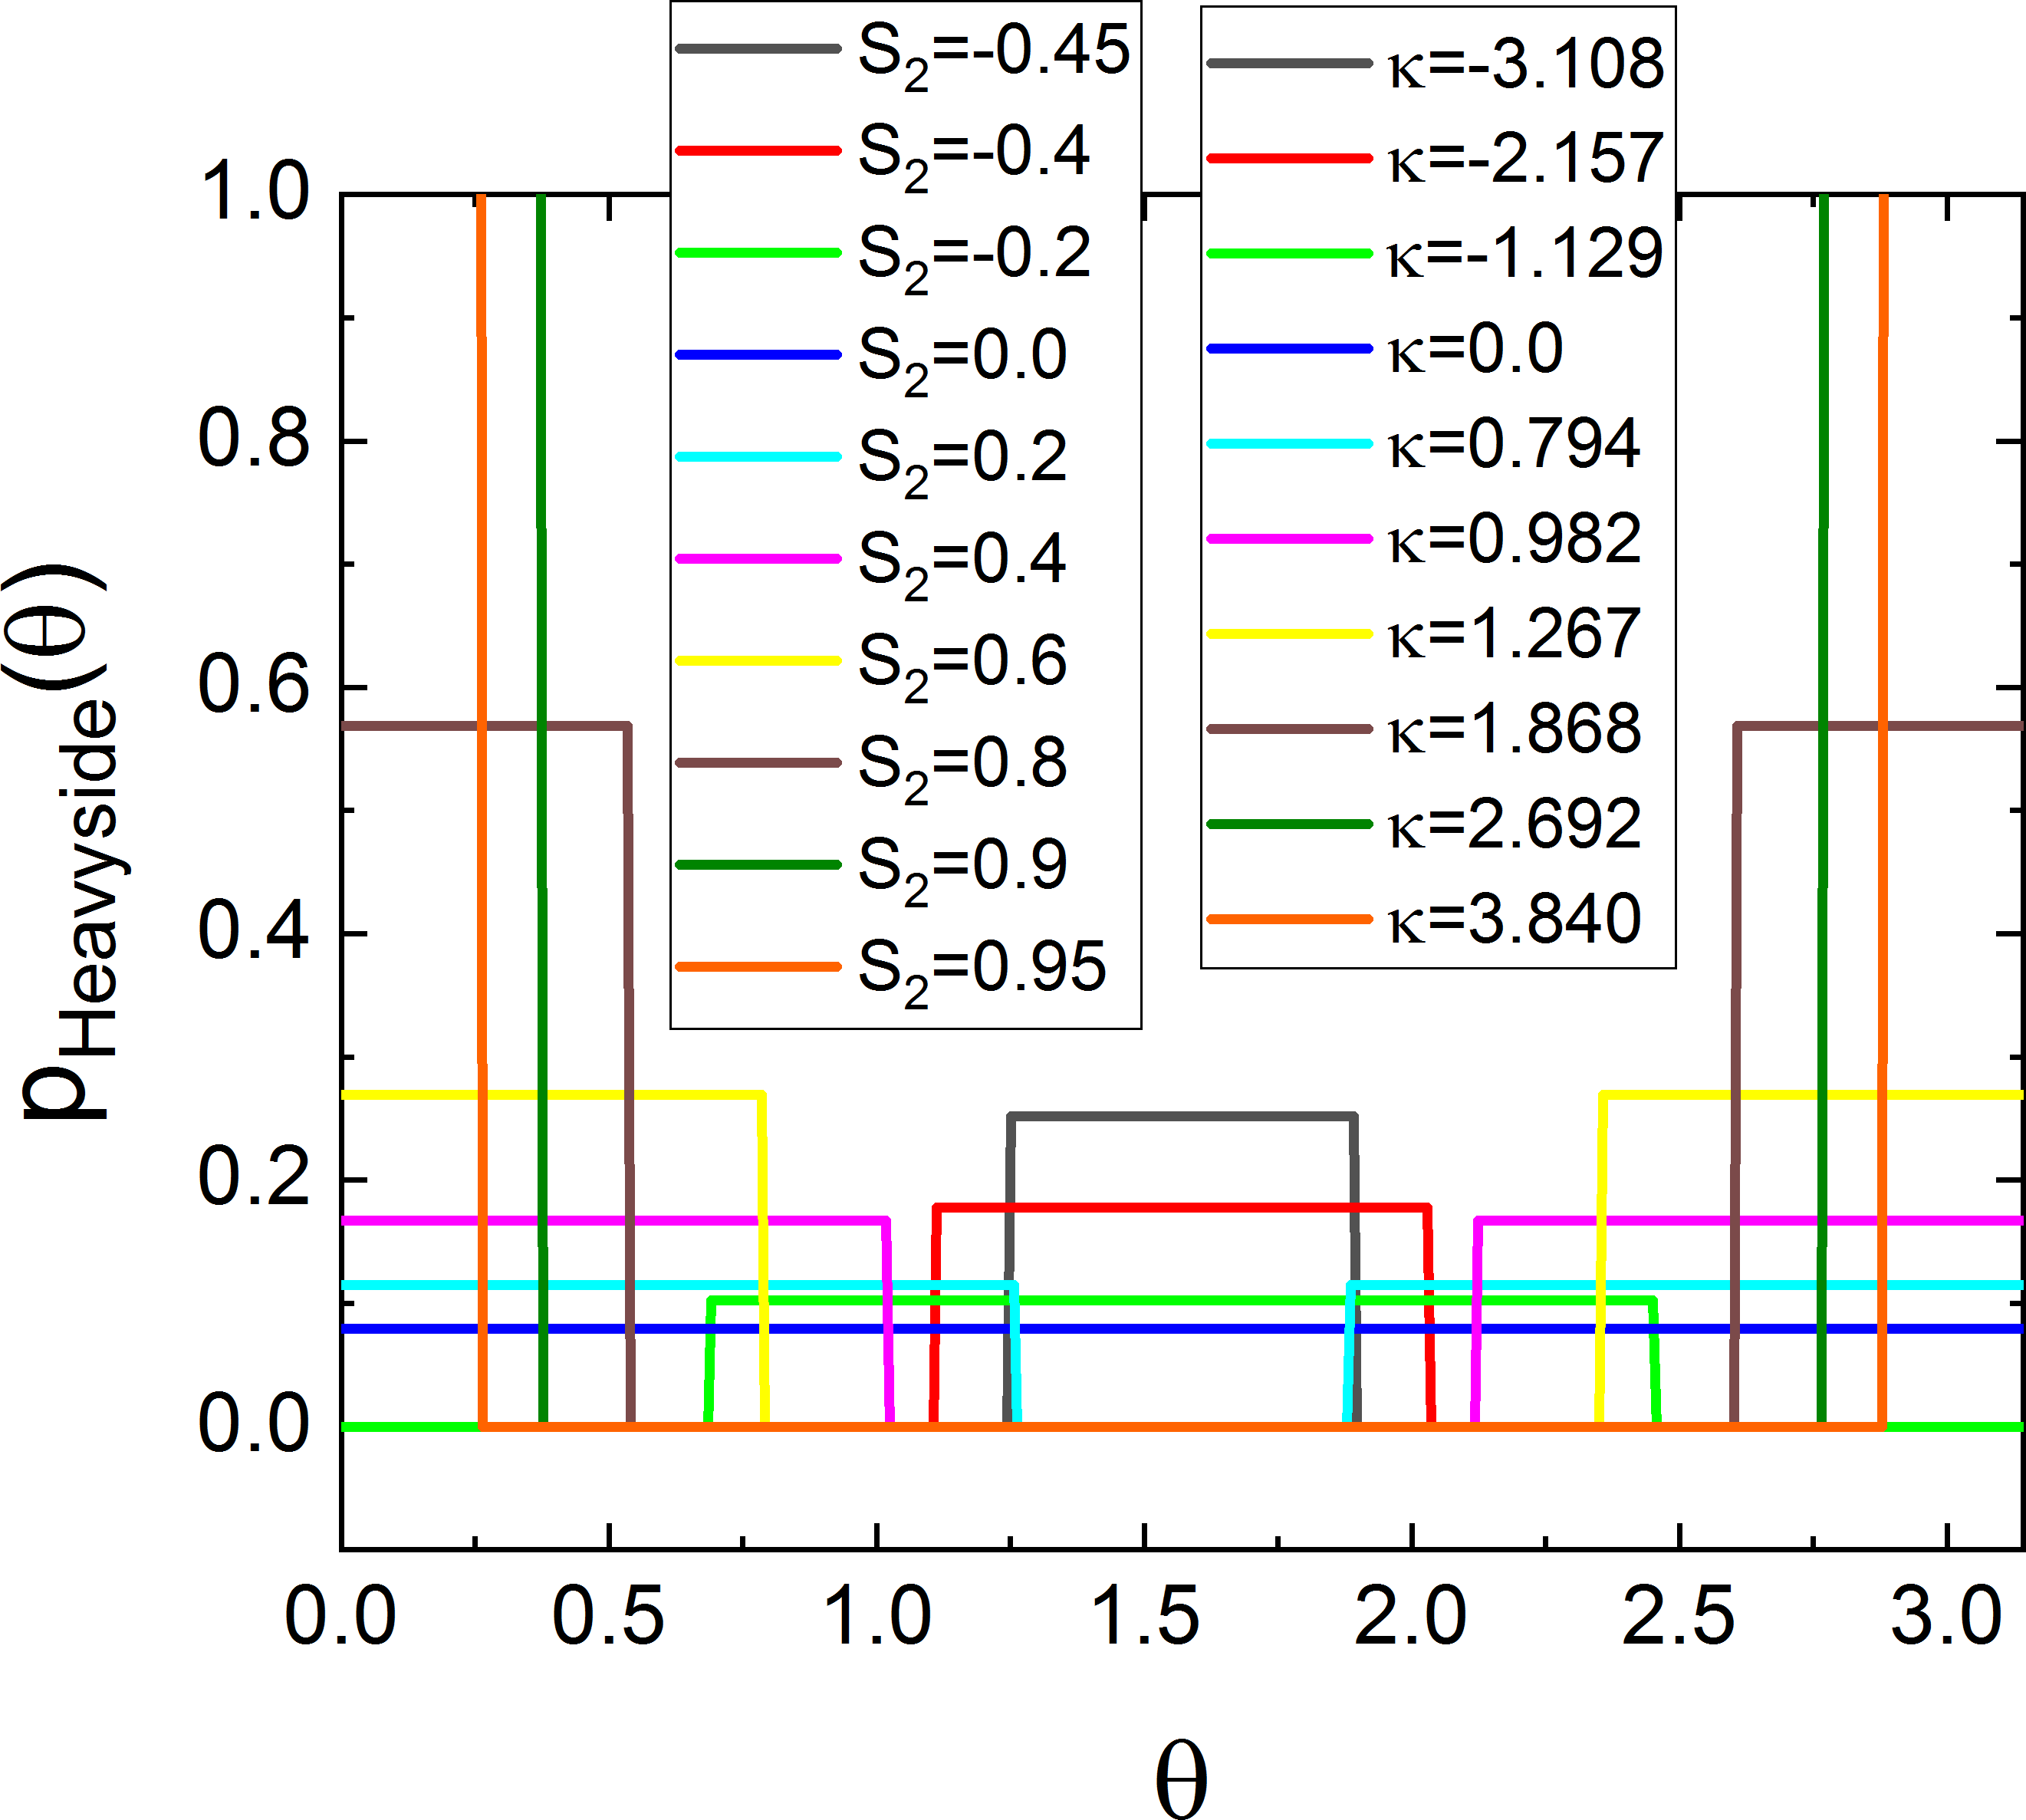
\includegraphics[width=0.75\textwidth]{../images/form_factor/cylindrical_obj/pHeavisideGr.png}
\caption{Heaviside orientation distribution $p_\mathrm{HS}(\theta,\kappa)$ for different values of $\kappa$, resulting in an order parameter as listed in table \ref{tab:kappas}.}
\label{fig:pHeavisideGr}
\end{figure}


\begin{align}
p(\theta,\phi;\kappa) & =
\begin{cases}
\displaystyle
\frac{1}{4\pi\left(1-\cos\left(1/\kappa\right)\right)}\left(\Pi\left(\frac{x\kappa}{2}\right) + \Pi\left(\frac{(x-\pi)\kappa}{2}\right)\right)
 & \mathrm{for~} \kappa >  \frac{2}{\pi}
 \\[5mm]
\displaystyle
 \frac{1}{4\pi} & \mathrm{for~}  \abs{\kappa} \leq \frac{2}{\pi}
 \\[5mm]
\displaystyle
 \frac{1}{4\pi\sin\left(\frac{1}{\abs{\kappa}}\right)} \Pi\left(\frac{\left(x-\frac{\pi}{2}\right)\abs{\kappa}}{2}\right) & \mathrm{for~}  \kappa<-\frac{2}{\pi}
\end{cases}
\end{align}
with the rectangle function $\Pi(x)$
\begin{align}
\Pi(x) &=
\begin{cases}
\displaystyle
0 & \mathrm{for~} \abs{x} > \frac12
 \\[5mm]
\displaystyle
\frac12 & \mathrm{for~}  \abs{x} = \frac12
 \\[5mm]
\displaystyle
 1 & \mathrm{for~}  \abs{x} < \frac12
\end{cases}
\end{align}

\vspace{5mm}

\underline{Input Parameters for model \texttt{Sheared Cylinders (Heaviside)}:}\\
\begin{description}
\item[\texttt{R}] radius of cylinders $R$
\item[\texttt{t}] shell thickness $t$
\item[\texttt{L}] cylinder length $L$
\item[\texttt{eta\_core}] scattering length density of cylinder core $\eta_\mathrm{core}$
\item[\texttt{eta\_shell}] scattering length density of cylinder shell $\eta_\mathrm{shell}$
\item[\texttt{eta\_solv}] scattering length density of solvent $\eta_\mathrm{solv}$
\item[\texttt{psi}] direction of scattering vector on the detector $\psi$
\item[{\texttt{sigma}}] width parameter of lognormal size distribution $\sigma$
\item[{\texttt{kappa}}] orientation distribution parameter $\kappa$
\end{description}

\vspace{5mm}

\underline{Input Parameters for model \texttt{Sheared Spheroids (Heaviside)}:}\\
\begin{description}
\item[\texttt{R\_equatorial}] equatorial semi-axes of spheroids $R_\mathrm{e}$
\item[\texttt{t}] shell thickness $t$
\item[\texttt{R\_polar}] polar semi-axis of spheroids $R_\mathrm{p}$
\item[\texttt{eta\_core}] scattering length density of cylinder core $\eta_\mathrm{core}$
\item[\texttt{eta\_shell}] scattering length density of cylinder shell $\eta_\mathrm{shell}$
\item[\texttt{eta\_solv}] scattering length density of solvent $\eta_\mathrm{solv}$
\item[\texttt{psi}] direction of scattering vector on the detector $\psi$
\item[{\texttt{sigma}}] width parameter of lognormal size distribution $\sigma$
\item[{\texttt{kappa}}] orientation distribution parameter $\kappa$
\end{description}

\vspace{5mm}

\underline{Note:}
\begin{itemize}
\item The size distribution is taken simultaneously over all parameters $R$, $t$, $L$, and $R_\mathrm{e}$, $t$, $R_\mathrm{p}$ respectively, so that their aspect ratios always stay constant.
\item For $\abs{\kappa}<\frac{2}{\pi}$ the partial derivative $\delta /\delta\kappa$ of the model function is zero which will cause an error message in the minimization routine. This means the fitting procedure will not work in this domain of values.
\end{itemize}


\clearpage
%%%%%%%%%%%%%%%%%%%%%%%%%%%%%%%%%%%%%%%%%%%%%%%%%%%%%%%%%%%%%%%%%%%%%%%%%%%%%%%%%%%%%%%%%%%%%
\section{anisotropic form factors of oriented primitive objects}
\label{ch:OPO}

In this section The scattering amplitudes of simple geometric objects are described having an arbitrary but fixed orientation as well as those which are obtained by an affine transformation. The most simple ones are unit spheres, unit cube and unit cylinder, and their affine deformed shapes of ellipsoid,  oblique parallelepiped and  oblique cylinder for which their $\B{Q}$-dependent form factors $F(\B{Q})$ are given analytically.

\noindent
\begin{figure}[htb]
\begin{subfigure}[b]{.3\textwidth}
   \centering
   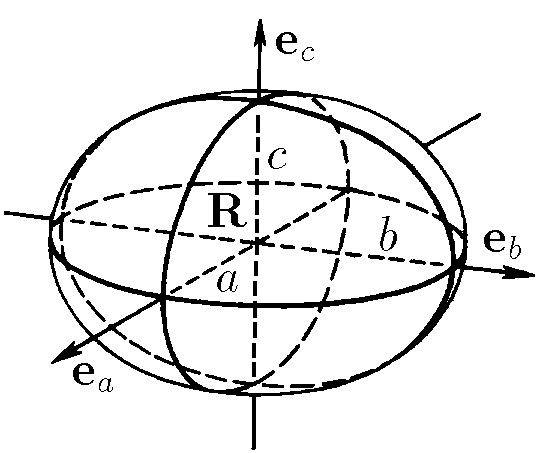
\includegraphics[width=\textwidth,height=0.8\textwidth]{ELLIPSE.png}
   \caption{ellipsoid}
   \label{fig:opo_ell}
\end{subfigure}
\hfill
\begin{subfigure}[b]{.3\textwidth}
   \centering
   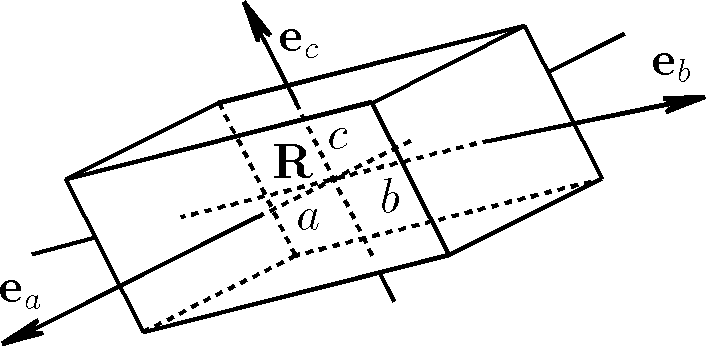
\includegraphics[width=\textwidth]{PAREPIP.png}
   \caption{parallelepiped}
   \label{fig:opo_parep}
\end{subfigure}
\hfill
\begin{subfigure}[b]{0.3\textwidth}
   \centering
   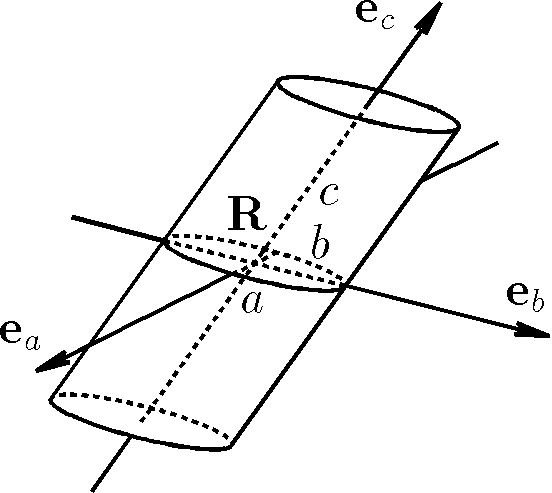
\includegraphics[width=\textwidth]{ZYLINDER.png}
   \caption{cylinder}
   \label{fig:opo_cyl}
\end{subfigure}
\caption{$\B{R}$: object center,
$a, b, c$: half axes/lengths,
$\B{e}_a$, $\B{e}_b$, $\B{e}_c$: directions of the half axes
}
\label{fig:opo}
\end{figure}

The scattering amplitude $F(\B{Q})$ of an object is given by the Fourier transform of the scattering length density distribution within the object
\begin{align}
F(\B{Q}) &= \int_V d\B{r}\, \eta(\B{r})\, e^{\imath \B{Qr}},
\end{align}
where $\eta(\B{r})$ is the scattering length density distribution of the scattering object and $V$ the sample volume.
In the following it is assumed that the particles have a homogeneous scattering length density
$\eta_P$, embedded in a matrix of also homogeneous scattering length density $\eta_M = \eta_P-\Delta\eta$.
The position, orientation and size of the objects is uniquely defined by the center of scattering length density $\B{R}$, the half axes $a$, $b$ and $c$, as well as the direction of the half axes $\B{e}_a$, $\B{e}_b$ and
$\B{e}_c$. The base vectors $\B{e}_i$ are normalized $\abs{\B{e}_i}=1$ but do not need to be orthogonal to each other.  For the scattering amplitude of an individual objects one gets after a translation by $-\B{R}$ and a following change of basis $\M{D}$ from cartesian coordinates
$O_{xyz} = \{\B{e}_x, \B{e}_y,\B{e}_z\}$
into the coordinate system of the particle $O_{abc}=\{a\B{e}_a, b\B{e}_b,
c\B{e}_c\}$, so that $\B{P}_{O_{abc}} = \M{D}\, \B{P}_{O_{xyz}}$
\begin{align}
F(\B{Q}) &=
e^{-\imath\B{QR}}\, \Delta\eta\,
\int\limits_{V(\B{0})} d\B{r}\, e^{\imath\B{Q}(\M{D}^{-1}\M{D}\B{r})}\\
%&=
%\det(\M{D}^{-1})\, e^{-\imath\B{QR}}\, \Delta\eta\,
%\int\limits_{\M{D} V(\B{0})} d\B{r}\, e^{\imath((\M{D}^{-1})^T\B{Q})\B{r}} \\
&=
\det(\M{D}^{-1})\, e^{-\imath\B{QR}}\, \Delta\eta\,
\int\limits_{\M{D} V(\B{0})} d\B{r}\, e^{\imath \B{\hat{Q}}\B{r}}
\end{align}
with
\begin{align}
\displaystyle \B{\hat{Q}} = (\M{D}^{-1})^T\,\B{Q}
= \left( \begin{array}{l} a\,\B{e}_a\B{Q}\\ b\,\B{e}_b\B{Q}\\
c\, \B{e}_c\B{Q}
\end{array}\right)
\label{eq:Q:dach}
\end{align}
$V(\B{0})$ is the volume of the scattering object a scattering lenth density center located at the origin of the coordinate system and $\M{D} V(\B{0})$ is the volume of the unit object, i.e. unit sphere, unit cube or unit cylinder.
The transformation matrix $\M{D}$ and its inverse $\M{D}^{-1}$ are given by
\begin{align}
\M{D}^{-1} &=
\left(
\begin{array}{ccc}
a\, e_{ax} & b\, e_{bx} & c\, e_{cx} \\
a\, e_{ay} & b\, e_{by} & c\, e_{cy} \\
a\, e_{az} & b\, e_{bz} & c\, e_{cz} \\
\end{array}
\right) = (a\B{e}_a,b\B{e}_b,c\B{e}_c)\\
 \B{Q}(\M{D}^{-1}\B{r}) &= ((\M{D}^{-1})^T\B{Q})\B{r} \U{,}\\
\det(\M{D}^{-1}) &= abc\,
( e_{ax}\, e_{by}\, e_{cz}
+ e_{ay}\, e_{bz}\, e_{cx}
+ e_{az}\, e_{bx}\, e_{cy} \nonumber \\
&\phantom{=} - e_{az}\, e_{by}\, e_{cx}
   - e_{ay}\, e_{bx}\, e_{cz}
   - e_{ax}\, e_{bz}\, e_{cy})
\end{align}
\begin{align}
\M{D} &= (\M{D}^{-1})^{-1} = \frac{1}{\det(\M{D}^{-1})}\,
          (\M{D}^{-1})^{\rm adj} \nonumber \\
&= \frac{1}{\det(\M{D}^{-1})} \, (b\B{e}_b\times c\B{e}_c,-a\B{e}_a
\times c\B{e}_c,a\B{e}_a\times b\B{e}_b)
\end{align}
whereas $\det(\M{D}) \, \det(\M{D}^{-1}) = \det(\M{D}\, \M{D}^{-1}) =\det(\idty) = 1$

To reorient or rotate the objects one simply changes the  direction of the base vectors $\B{e}_a$, $\B{e}_b$, $\B{e}_c$ which is done by introducing a rotation matrix $\M{R}_{\alpha\beta\gamma}$. The rotation matrix can be defined via Euler angles $\alpha$, $\beta$,and $\gamma$. Its definition depends on the convention. There exist twelve possible sequences of rotation axes, divided in two groups: proper Euler angles ($z$-$x$-$z$, $x$-$y$-$x$, $y$-$z$-$y$, $z$-$y$-$z$, $x$-$z$-$x$, $y$-$x$-$y$),
Tait–Bryan angles ($x$-$y$-$z$, $y$-$z$-$x$, $z$-$x$-$y$, $x$-$z$-$y$, $z$-$y$-$x$, $y$-$x$-$z$). The difference between the two conventions is that Tait–Bryan angles represent rotations about three distinct axes, while proper Euler angles use the same axis for both the first and third elemental rotations. \SASfit allows internally to use any of the 12 conventions. However, as default conventions the yaw-pitch-roll is used (also named gier-nick-roll, east-north-up, north-East-Down, or $z$-$y$-$x$),  so that
\begin{align}
\displaystyle \B{\hat{Q}} &=
  \left( \begin{array}{l} a\,\M{R}_{\alpha\beta\gamma}\B{e}_a\B{Q}\\
                          b\,\M{R}_{\alpha\beta\gamma}\B{e}_b\B{Q}\\
                          c\,\M{R}_{\alpha\beta\gamma}\B{e}_c\B{Q}
\end{array}\right)
\label{eq:Q:dach}
\end{align}
\vspace{5mm}

Next to the form factor of an oriented primitive object also the form factor of it fully randomly oriented version is made available. The orientational average is done by integrating over the full Ewald's sphere, which is a double integration. \SASfit supplies for this orientational average separate integration routines which can be configured via the GUI. Next to the multidimensional adaptive integration routines \texttt{pcubature} and \texttt{hcubature} from \cite{Johnson} also some other routines are supplied, which however are nonadaptive without error estimate of the integral but optimized for integrations over a sphere surface. Nevertheless, these routines often need significant less function evaluations than a conventional multidimensional integration routines. The implemented methods are a 2D-GaussLegendre integration, Lebedev \cite{Lebedev1975,Lebedev1976,Lebedev1977} and Fibonacci \cite{Niederreiter1992,Marques2013} quadrature algorithm with a fixed and configurable number of function evaluations and without error estimation of the integral.

\subsection{perfect and random oriented ellipsoid} ~\\

\begin{figure}[htb]
\begin{center}
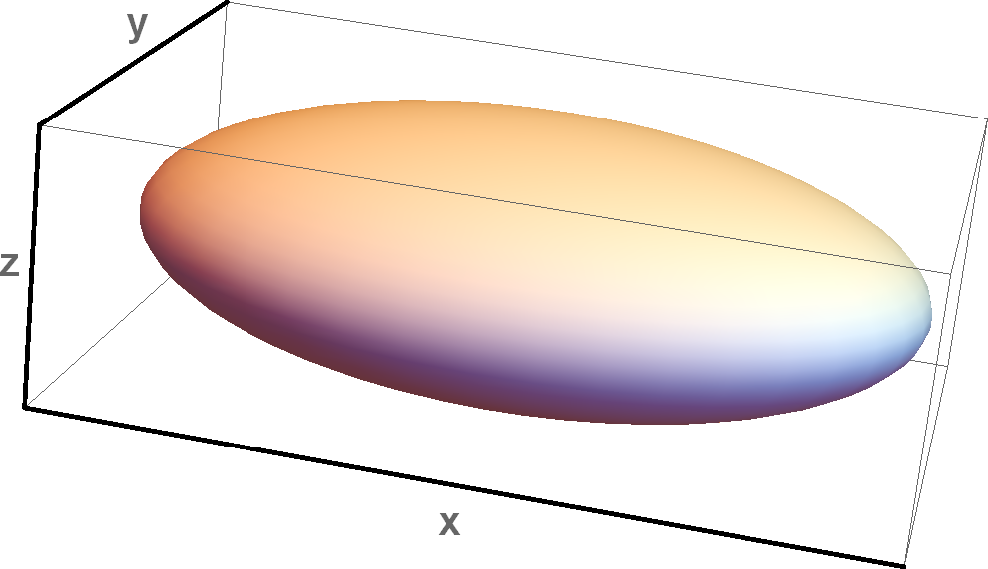
\includegraphics[width=0.65\textwidth]{../images/form_factor/supershapes/triaxial_ellipsoid321.png}
\end{center}
\caption{ellipsoid with semi-axis $(a:b:c)=(3:2:1)$ and $\alpha=\beta=\gamma=0$}
\label{fig:opo_ellipsoid}
\end{figure}

This form factor describes an oblique ellipsoid with half axis $a$, $b$, and $c$, which is obtained by an affine transformation of an unit sphere. The detector plane is in the $xy$-plane and the incident beam in the $-z$-direction. The unit vectors $\B{e}_a$, $\B{e}_b$, and $\B{e}_c$ are assumed in this example pointing into the directions of the three orthogonal axis $\B{e}_x$, $\B{e}_y$, and $\B{e}_z$ and therefore represent a triaxial ellipsoid.


\begin{align}
F_E(\B{Q}) &=
\det(\M{D}^{-1})\, e^{-\imath\B{QR}}\, \Delta\eta\, \int\limits_0^1
dr\, r^2 \int\limits_0^{\pi} d\theta\, \sin \theta \int\limits_0^{2\pi}
d\phi \, e^{\imath\B{\hat{Q}r}} \nonumber \\
&=
\displaystyle 4\, \pi\, \det(\M{D}^{-1})\, e^{-\imath\B{QR}}\,
\Delta\eta\, \frac{\sin \abs{\B{\hat{Q}}}-
\abs{\B{\hat{Q}}}\cos \abs{\B{\hat{Q}}}}{\abs{\B{\hat{Q}}}^3}
\label{eq:form:E}
\end{align}
For a random oriented ellipsoid one either can integrate over all Euler-angle, which is a tripple integration or over all orientations of $\B{Q}$, which is a double integration and performed for the randomized form factor. The corresponding scattering amplitude $F_{\mathrm{E},rnd}$ and scattering intensity $P_{\mathrm{E},rnd}$ are then given by
\begin{align}
F_{\mathrm{E},rnd}(Q) &= \left\langle F_E(\B{Q})\right\rangle_\B{Q} = \int_0^\pi\mathrm{d}\theta \int_0^{2\pi}\mathrm{d}\phi \; F_E\left(Q\begin{pmatrix}
                                       \cos(\phi)\sin(\theta) \\
                                       \sin(\phi)\sin(\theta) \\
                                       \cos(\theta)
                                     \end{pmatrix}\right) \\
P_{\mathrm{E},rnd}(Q) &= \left\langle F_E^2(\B{Q})\right\rangle_\B{Q} = \int_0^\pi\mathrm{d}\theta \int_0^{2\pi}\mathrm{d}\phi \; F_E^2\left(Q\begin{pmatrix}
                                       \cos(\phi)\sin(\theta) \\
                                       \sin(\phi)\sin(\theta) \\
                                       \cos(\theta)
                                     \end{pmatrix}\right) 
\end{align}

\begin{figure}[htb]
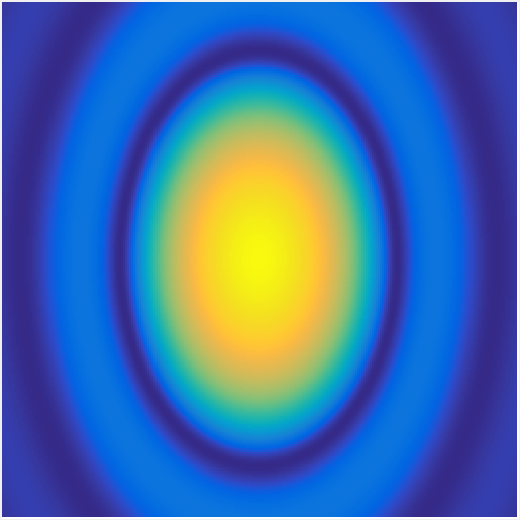
\includegraphics[width=0.31\textwidth]{../images/form_factor/supershapes/ellipsoid_0_0_0_18m.png} \hfill
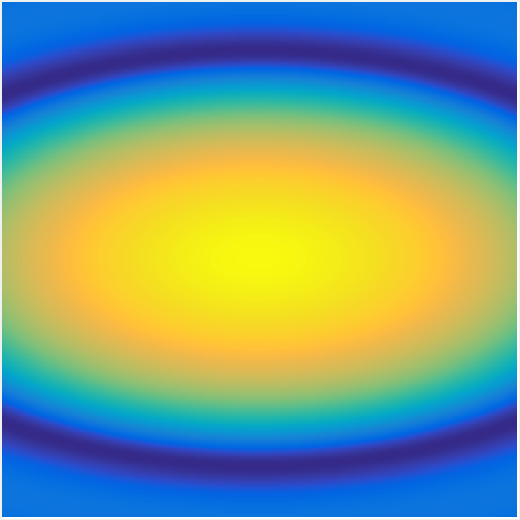
\includegraphics[width=0.31\textwidth]{../images/form_factor/supershapes/ellipsoid_0_90_0_18m.png}  \hfill 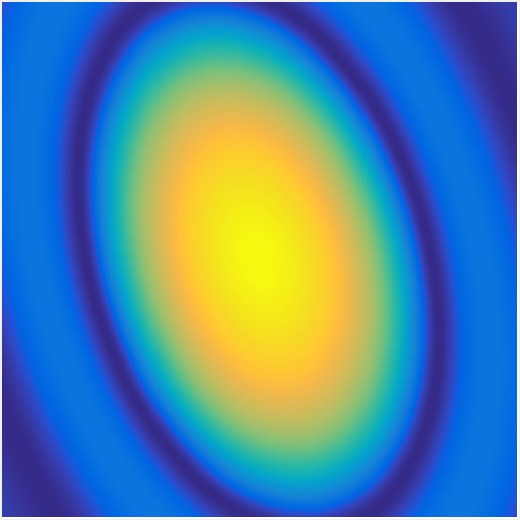
\includegraphics[width=0.31\textwidth]{../images/form_factor/supershapes/ellipsoid_0_45_45_18m.png}
\caption{Scattering patterns at 18m detector distance and a wavelength of $\lambda=0.6$nm. The ellipsoids are simulated with radii of $a=30$nm, $b=20$nm, and $c=10$nm. The Tait–Bryan angles (yaw-pitch-roll) are $(\alpha=0^\circ,\beta=0^\circ,\gamma=0^\circ)$, $(\alpha=0^\circ,\beta=90^\circ,\gamma=0^\circ)$, and $(\alpha=0^\circ,\beta=45^\circ,\gamma=45^\circ)$ }
\label{fig:opo_ellipsoidIQ2D}
\end{figure}

~\\
\underline{Input Parameters for model \texttt{ellipsoid (opo)}:}
\begin{description}
\item[\texttt{a}] length of first axis
\item[\texttt{ea\_x}] $x$-component of fist axis.
\item[\texttt{ea\_y}] $y$-component of fist axis.
\item[\texttt{ea\_z}] $z$-component of fist axis.
\item[\texttt{b}] length of second axis
\item[\texttt{eb\_x}] $x$-component of second axis.
\item[\texttt{eb\_y}] $y$-component of second axis.
\item[\texttt{eb\_z}] $z$-component of fsecondist axis.
\item[\texttt{c}] length of third axis
\item[\texttt{ec\_x}] $x$-component of third axis.
\item[\texttt{ec\_y}] $y$-component of third axis.
\item[\texttt{ec\_z}] $z$-component of third axis.
\item[\texttt{eta\_p}] scattering length density $\eta_p$ of particle
\item[\texttt{eta\_m}] scattering length density $\eta_m$ of matrix
\item[\texttt{alpha}] first Euler angle
\item[\texttt{beta}] second Euler angle
\item[\texttt{gamma}] third Euler angle
\item[\texttt{psi}] direction of $\B{Q}$ on detector ($\psi=0$, $x$-direction, to the right)
\end{description}

~\\
\underline{Input Parameters for model \texttt{ellipsoid (opo, random)}:}
\begin{description}
\item[\texttt{a}] length of first axis
\item[\texttt{ea\_x}] $x$-component of fist axis.
\item[\texttt{ea\_y}] $y$-component of fist axis.
\item[\texttt{ea\_z}] $z$-component of fist axis.
\item[\texttt{b}] length of second axis
\item[\texttt{eb\_x}] $x$-component of second axis.
\item[\texttt{eb\_y}] $y$-component of second axis.
\item[\texttt{eb\_z}] $z$-component of fsecondist axis.
\item[\texttt{c}] length of third axis
\item[\texttt{ec\_x}] $x$-component of third axis.
\item[\texttt{ec\_y}] $y$-component of third axis.
\item[\texttt{ec\_z}] $z$-component of third axis.
\item[\texttt{eta\_p}] scattering length density $\eta_p$ of particle
\item[\texttt{eta\_m}] scattering length density $\eta_m$ of matrix
\end{description}

\noindent\underline{Note:}
\begin{itemize}
\item the unit vector $\B{e}_a$, $\B{e}_b$, and $\B{e}_c$ are internally normalized to 1 and need to be orthogonal to each other.
\end{itemize}

\subsection{oriented parallelepiped} ~\\

\begin{figure}[htb]
\begin{center}
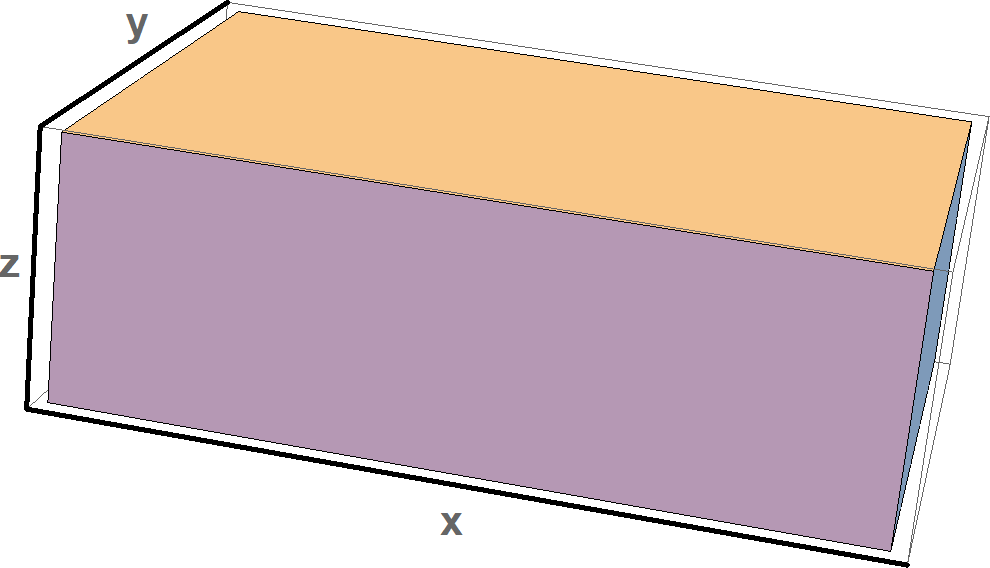
\includegraphics[width=0.6\textwidth]{../images/form_factor/supershapes/parallel_epiped321.png}
\end{center}
\caption{parallelepiped with half edge length $(a:b:c)=(3:2:1)$ and $\alpha=\beta=\gamma=0$}
\label{fig:opo_cube}
\end{figure}

This form factor describes an oblique parallelepiped which is obtained by an affine transformation of an unit cube with half edge lengths of $a$, $b$, and $c$. The detector plane is in the $xy$-plane and the incident beam in the $-z$-direction.


\begin{align}
F_P(\B{Q}) &=
\det(\M{D}^{-1})\, e^{-\imath\B{QR}}\, \Delta\eta\, \int\limits_{-1}^1
dx\, \int\limits_{-1}^{1} dy\, \int\limits_{-1}^{1} dz\,
e^{\imath\B{\hat{Q}r}} \nonumber \\
&= \displaystyle
8\, \det(\M{D}^{-1})\, e^{-\imath\B{QR}} \,\Delta\eta\,
\frac{\sin \B{\hat{Q}}\, \B{e}_x}{\B{\hat{Q}}\, \B{e}_x}
\,
\frac{\sin \B{\hat{Q}}\, \B{e}_y}{\B{\hat{Q}}\, \B{e}_y}
\,
\frac{\sin \B{\hat{Q}}\, \B{e}_z}{\B{\hat{Q}}\, \B{e}_z}
\label{eq:form:P}
\end{align}


\begin{figure}[htb]
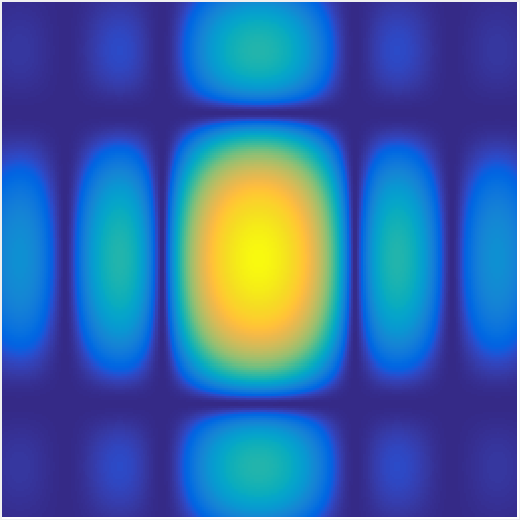
\includegraphics[width=0.31\textwidth]{../images/form_factor/supershapes/parallelepiped_0_0_0_18m.png}
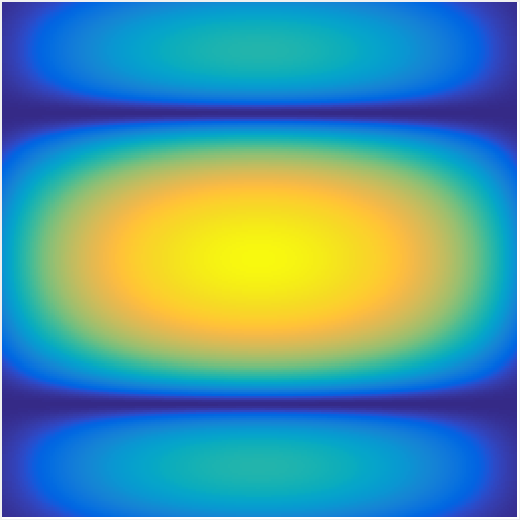
\includegraphics[width=0.31\textwidth]{../images/form_factor/supershapes/parallelepiped_0_90_0_18m.png}   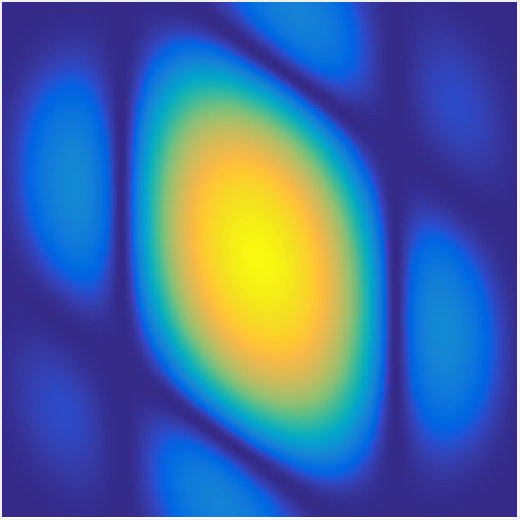
\includegraphics[width=0.31\textwidth]{../images/form_factor/supershapes/parallelepiped_0_45_45_18m.png}
\caption{Scattering patterns at 18m detector distance and a wavelength of $\lambda=0.6$nm. The parallelepipeds are simulated with half edge length of $a=30$nm, $b=20$nm, and $c=10$nm. The Tait–Bryan angles (yaw-pitch-roll) are $(\alpha=0^\circ,\beta=0^\circ,\gamma=0^\circ)$, $(\alpha=0^\circ,\beta=90^\circ,\gamma=0^\circ)$, and $(\alpha=0^\circ,\beta=45^\circ,\gamma=45^\circ)$ }
\label{fig:opo_parallelepipedIQ2D}
\end{figure}

\subsection{oriented cylinder} ~\\

\begin{figure}[htb]
\begin{center}
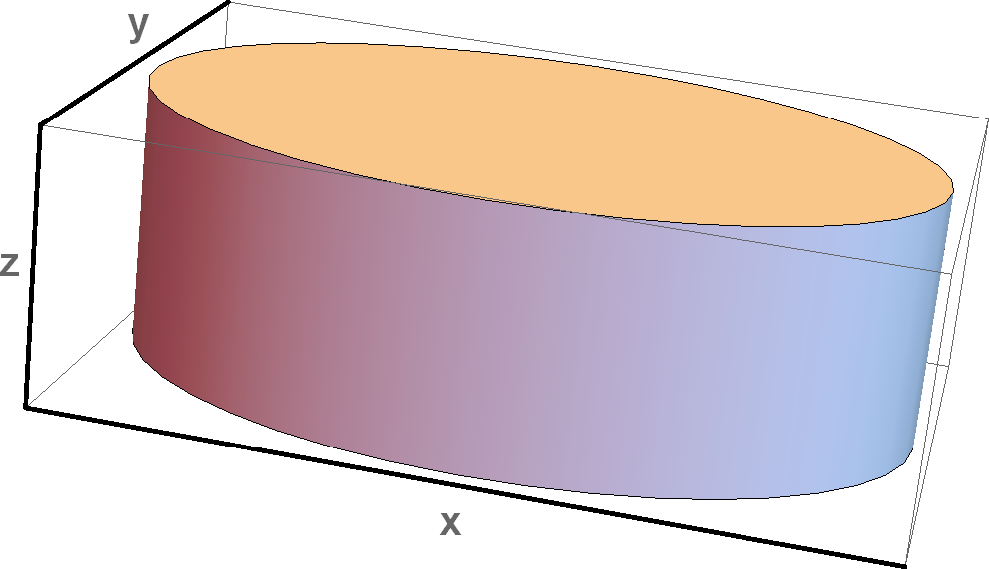
\includegraphics[width=0.6\textwidth]{../images/form_factor/supershapes/cylinder321.png}
\end{center}
\caption{cylinder with radii $a$ and $b$ and half height $c$. The axis ratios of the cylinder shown are $(a:b:c)=(3:2:1)$ and $\alpha=\beta=\gamma=0$}
\label{fig:opo_cylinder}
\end{figure}

This form factor describes an oblique parallelepiped which is obtained by an affine transformation of an unit cylinder with radii $a$ and $b$ and half height $c$. The detector plane is in the $xy$-plane and the incident beam in the $-z$-direction.


\begin{align}
F_C(\B{Q}) &=
\det(\M{D}^{-1})\, e^{-\imath\B{QR}}\, \Delta\eta\, \int\limits_{-1}^1
dz\, \int\limits_{0}^{1} dr\, r\, \int\limits_{0}^{2\pi} d\phi \,
e^{\imath\B{\hat{Q}r}} \nonumber \\
&=
4\, \pi\, \det(\M{D}^{-1})\, e^{-\imath\B{QR}}\, \Delta\eta\,
\frac{\sin\B{\hat{Q}e}_z}{\B{\hat{Q}e}_z}
\int\limits_{0}^1 dr\,r\,
\U{J}_0\left(r\, \sqrt{\left(\B{\hat{Q}}\B{e}_x\right)^2+
\left(\B{\hat{Q}}\B{e}_y\right)^2}\right)
\nonumber \\
&= \displaystyle
8\, \pi\,\det(\M{D}^{-1})\, e^{-\imath\B{QR}}\,
\Delta\eta\, \frac{\sin\B{\hat{Q}}\B{e}_z}{\B{\hat{Q}}\B{e}_z}
\, \frac{\U{J}_1\left(\sqrt{\left(\B{\hat{Q}}\B{e}_x\right)^2+
\left(\B{\hat{Q}}\B{e}_y\right)^2}\right)}{\sqrt{
\left(\B{\hat{Q}}\B{e}_x\right)^2+\left(\B{\hat{Q}}\B{e}_y\right)^2}}
\label{eq:form:C}
\end{align}

\begin{figure}[htb] 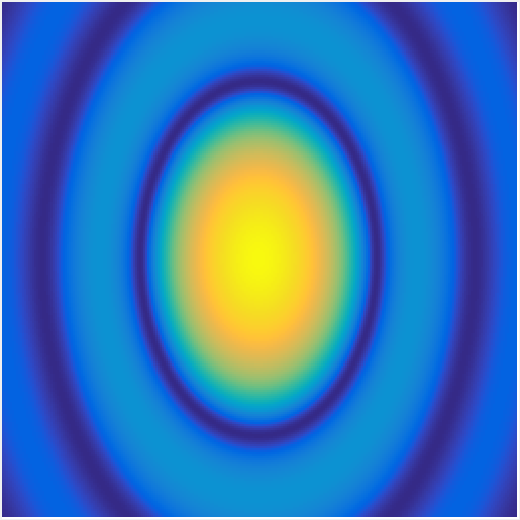
\includegraphics[width=0.31\textwidth]{../images/form_factor/supershapes/cylinder_0_0_0_18m.png}
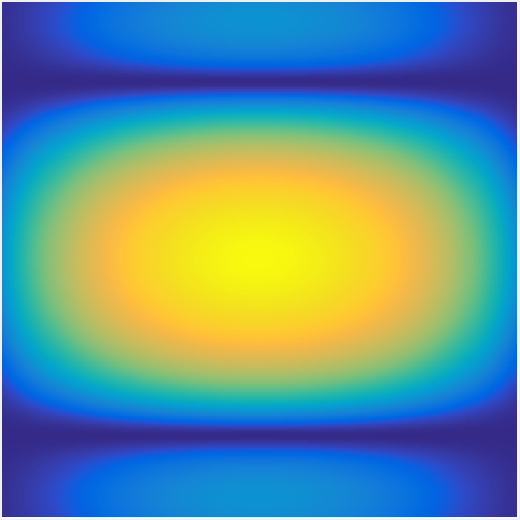
\includegraphics[width=0.31\textwidth]{../images/form_factor/supershapes/cylinder_0_90_0_18m.png}   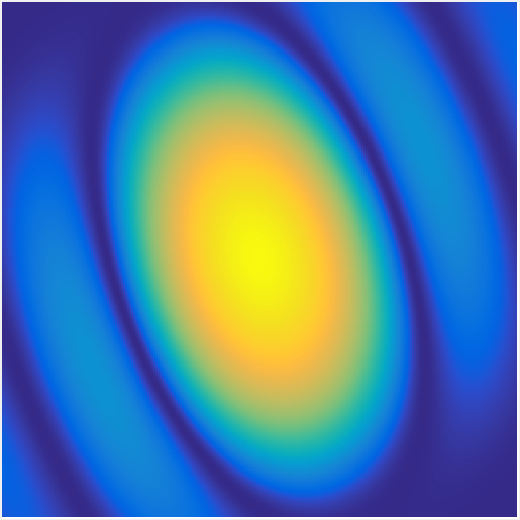
\includegraphics[width=0.31\textwidth]{../images/form_factor/supershapes/cylinder_0_45_45_18m.png}
\caption{Scattering patterns at 18m detector distance and a wavelength of $\lambda=0.6$nm. The cylinders are simulated with radii of $a=30$nm, $b=20$nm, and half height length $c=10$nm. The Tait–Bryan angles (yaw-pitch-roll) are $(\alpha=0^\circ,\beta=0^\circ,\gamma=0^\circ)$, $(\alpha=0^\circ,\beta=90^\circ,\gamma=0^\circ)$, and $(\alpha=0^\circ,\beta=45^\circ,\gamma=45^\circ)$ }
\label{fig:opo_cylinderIQ2D}
\end{figure}



\subsection{oriented super-quadrics} ~\\

\begin{figure}[htb]
\begin{tabular}{ccccc}
  $\epsilon_1=0.1$
    & 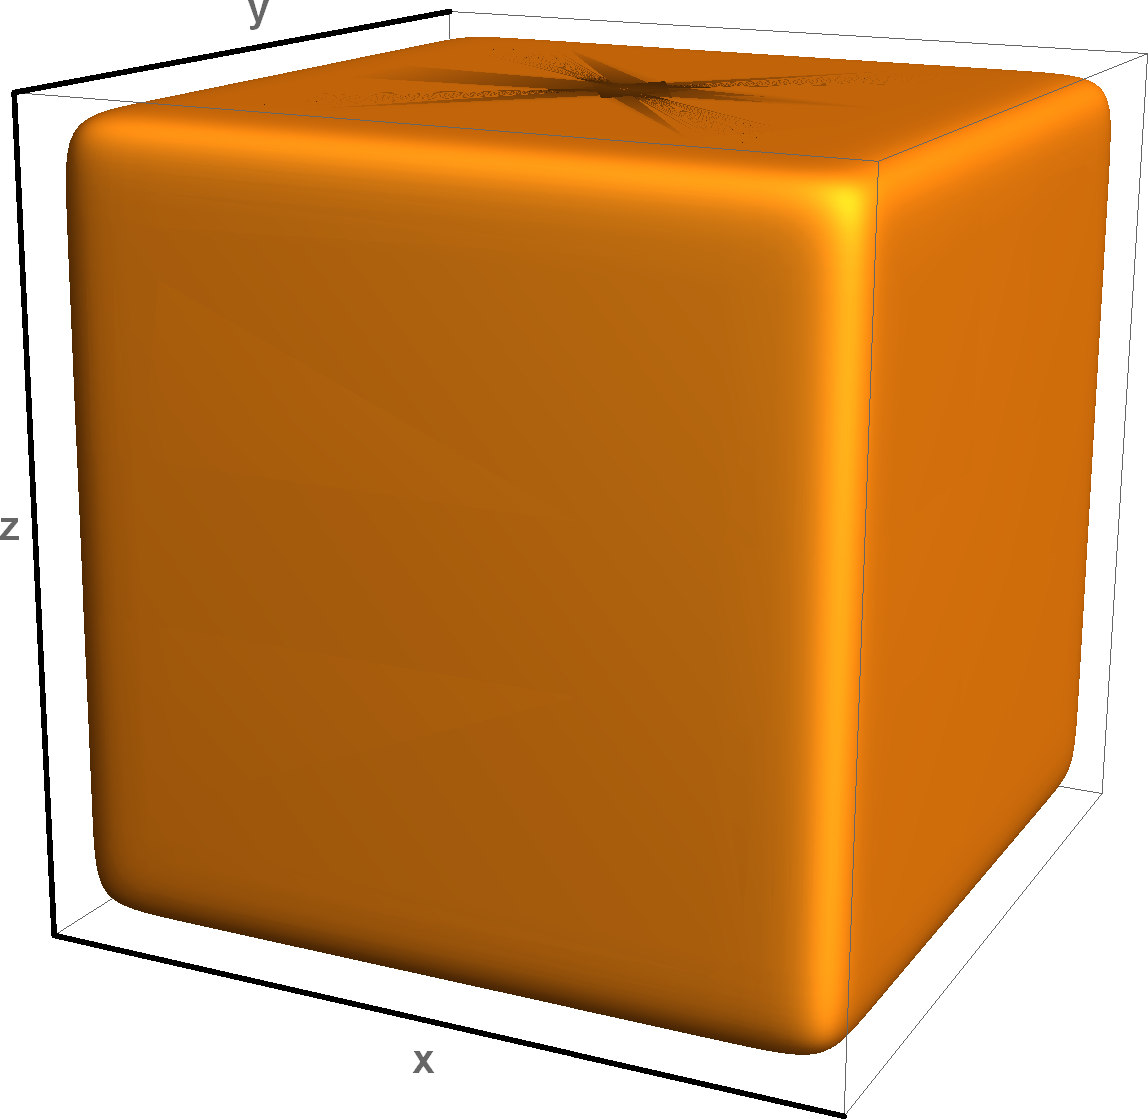
\includegraphics[width=0.2\textwidth]{../images/form_factor/supershapes/superquadric111_01_01.png}
    & 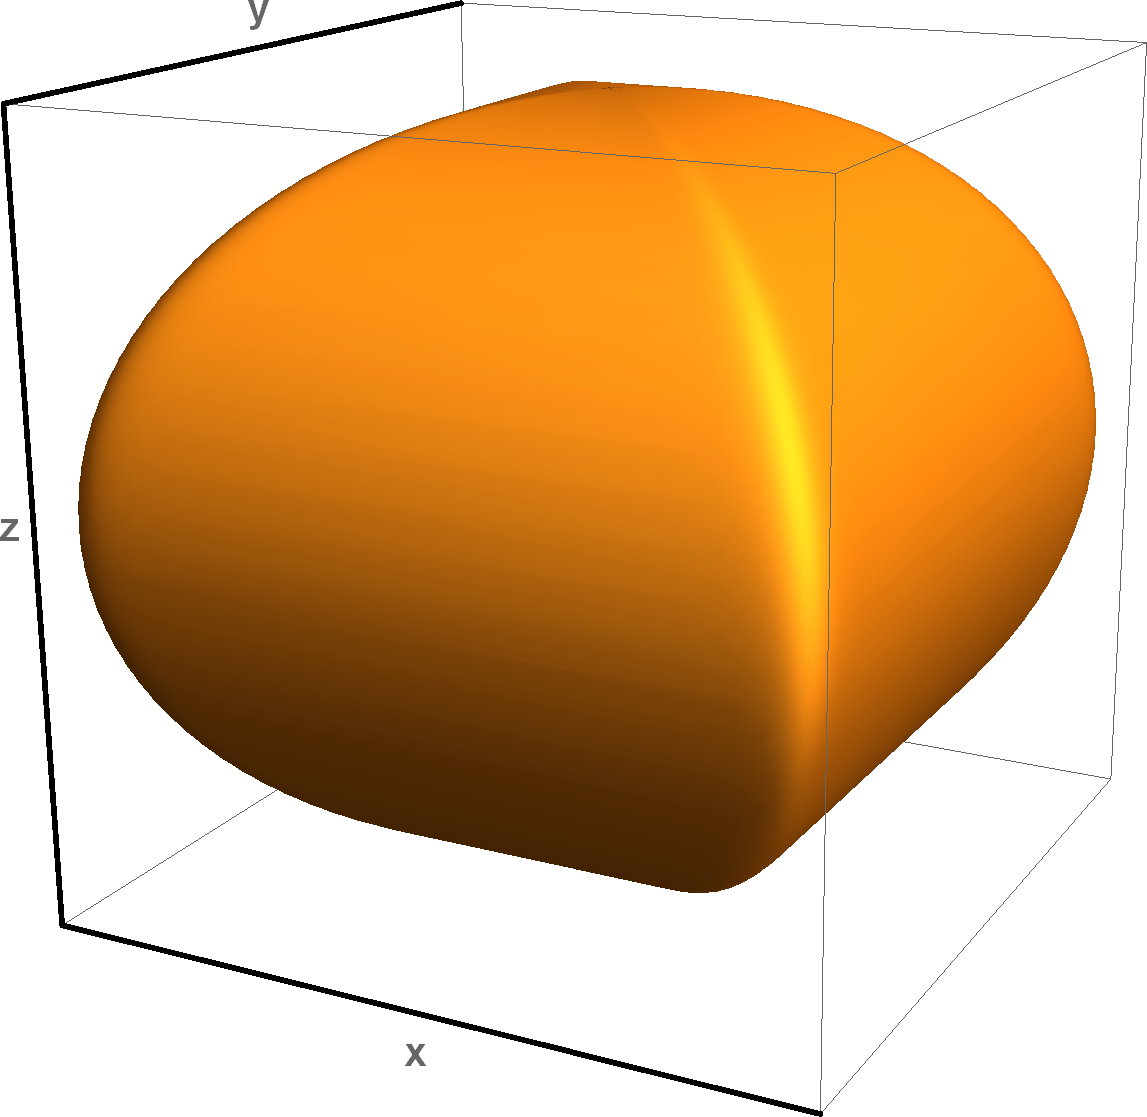
\includegraphics[width=0.2\textwidth]{../images/form_factor/supershapes/superquadric111_01_1.png}
    & 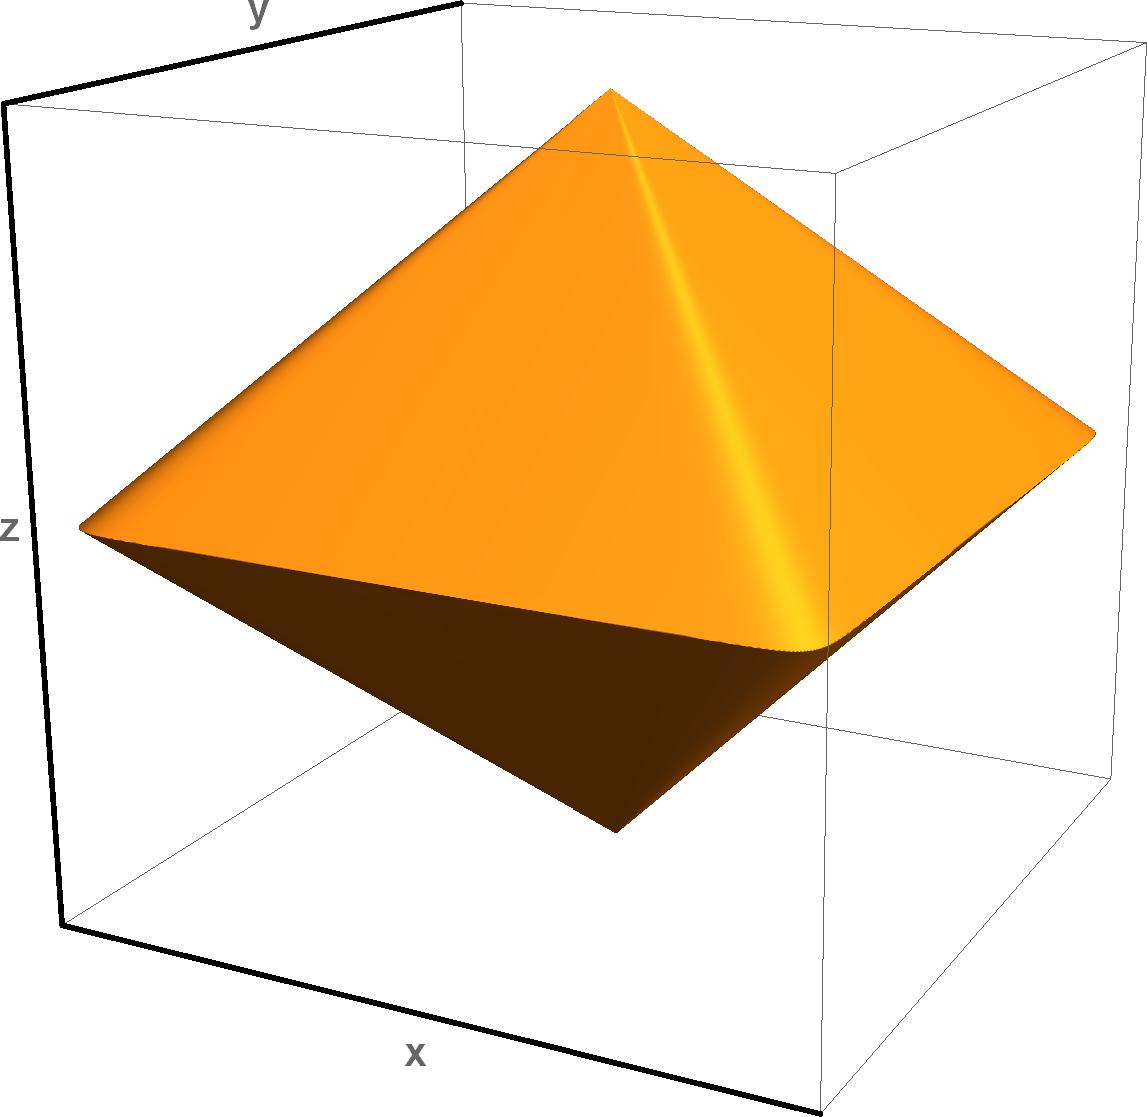
\includegraphics[width=0.2\textwidth]{../images/form_factor/supershapes/superquadric111_01_2.png}
    & 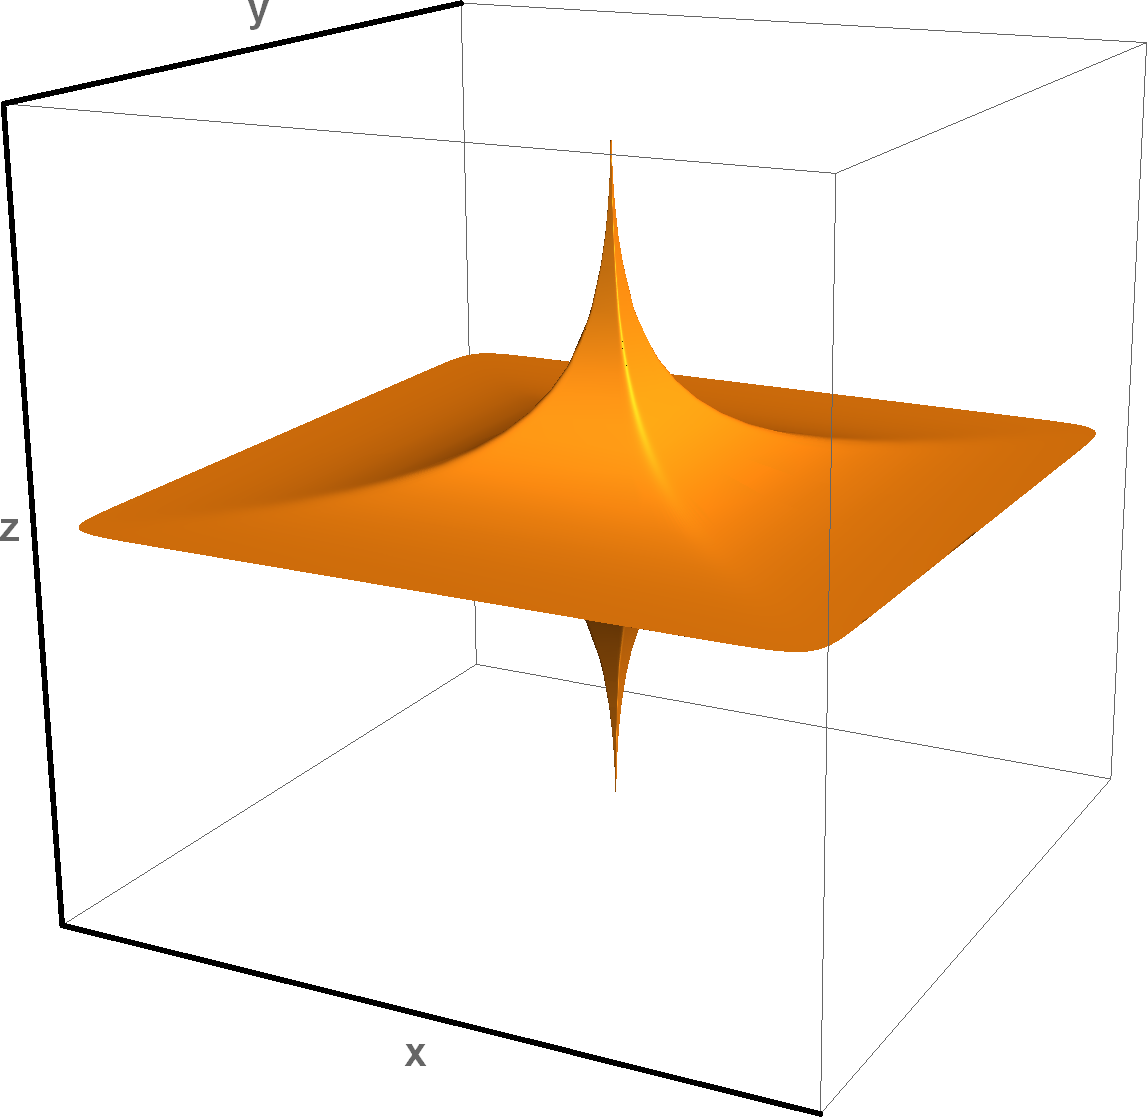
\includegraphics[width=0.2\textwidth]{../images/form_factor/supershapes/superquadric111_01_5.png} \\
  $\epsilon_1=1$
    & 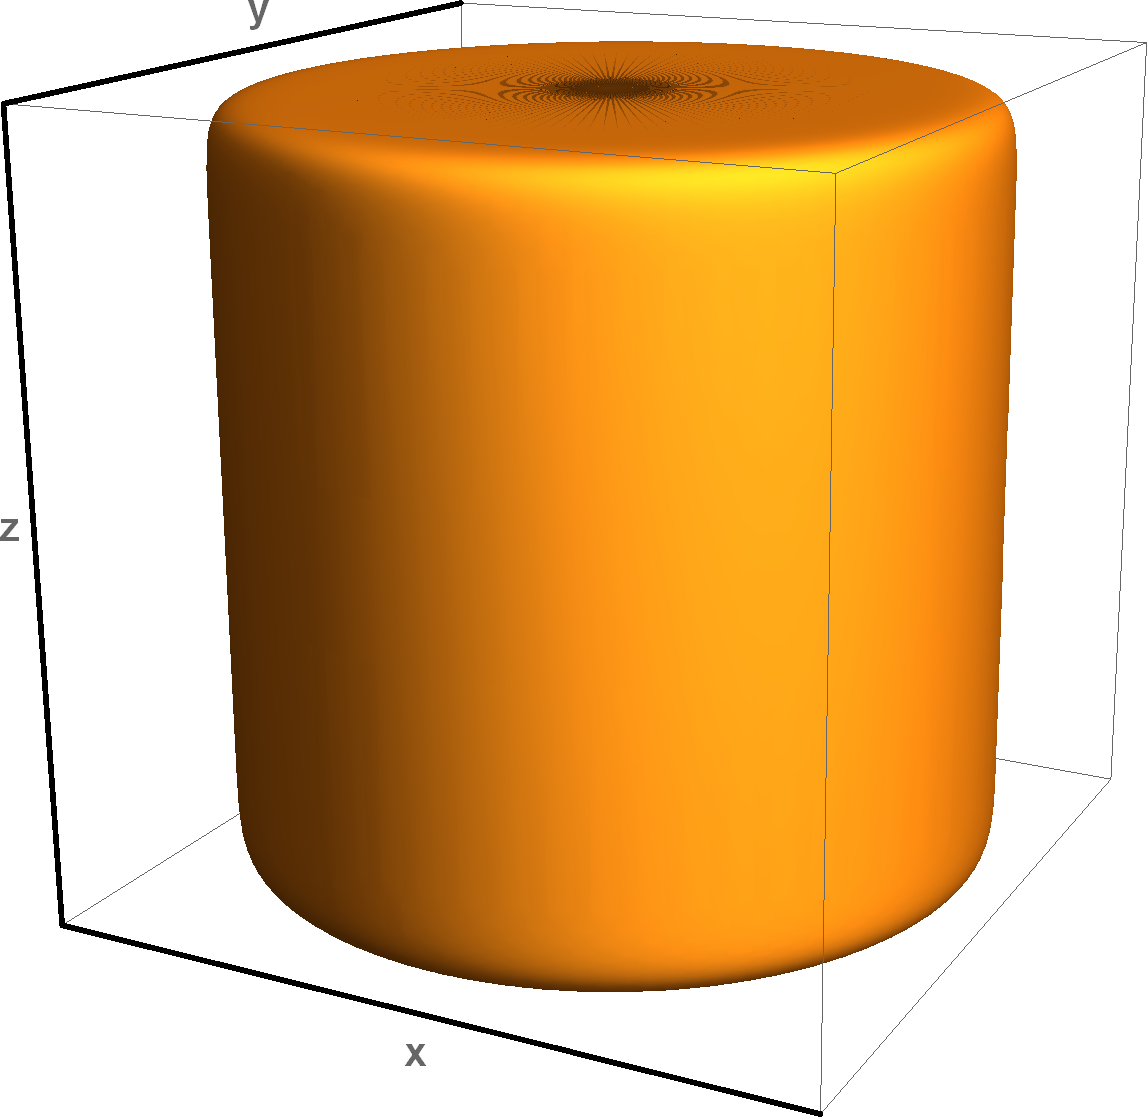
\includegraphics[width=0.2\textwidth]{../images/form_factor/supershapes/superquadric111_1_01.png}
    & 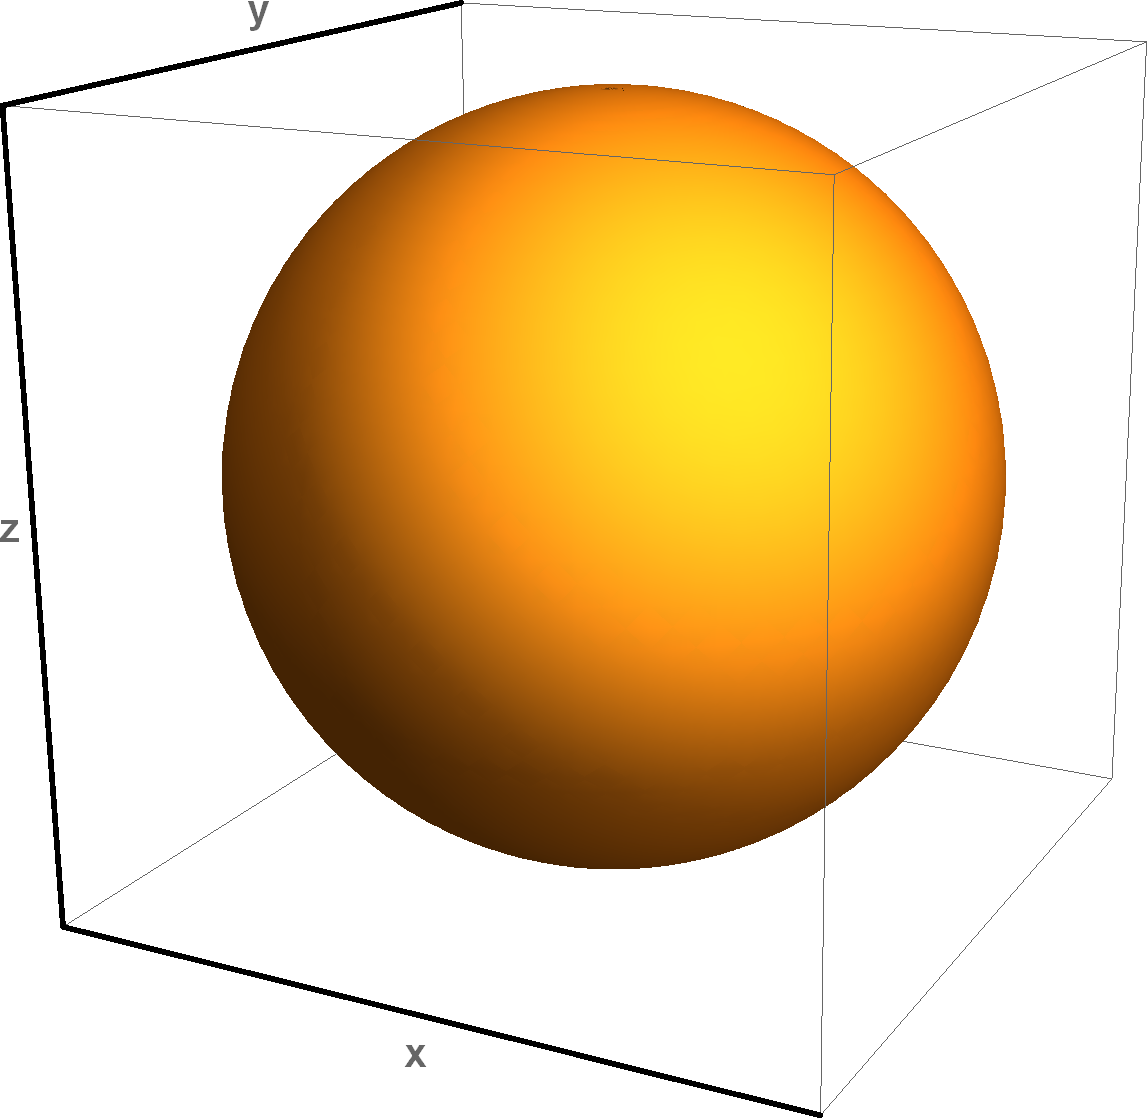
\includegraphics[width=0.2\textwidth]{../images/form_factor/supershapes/superquadric111_1_1.png}
    & 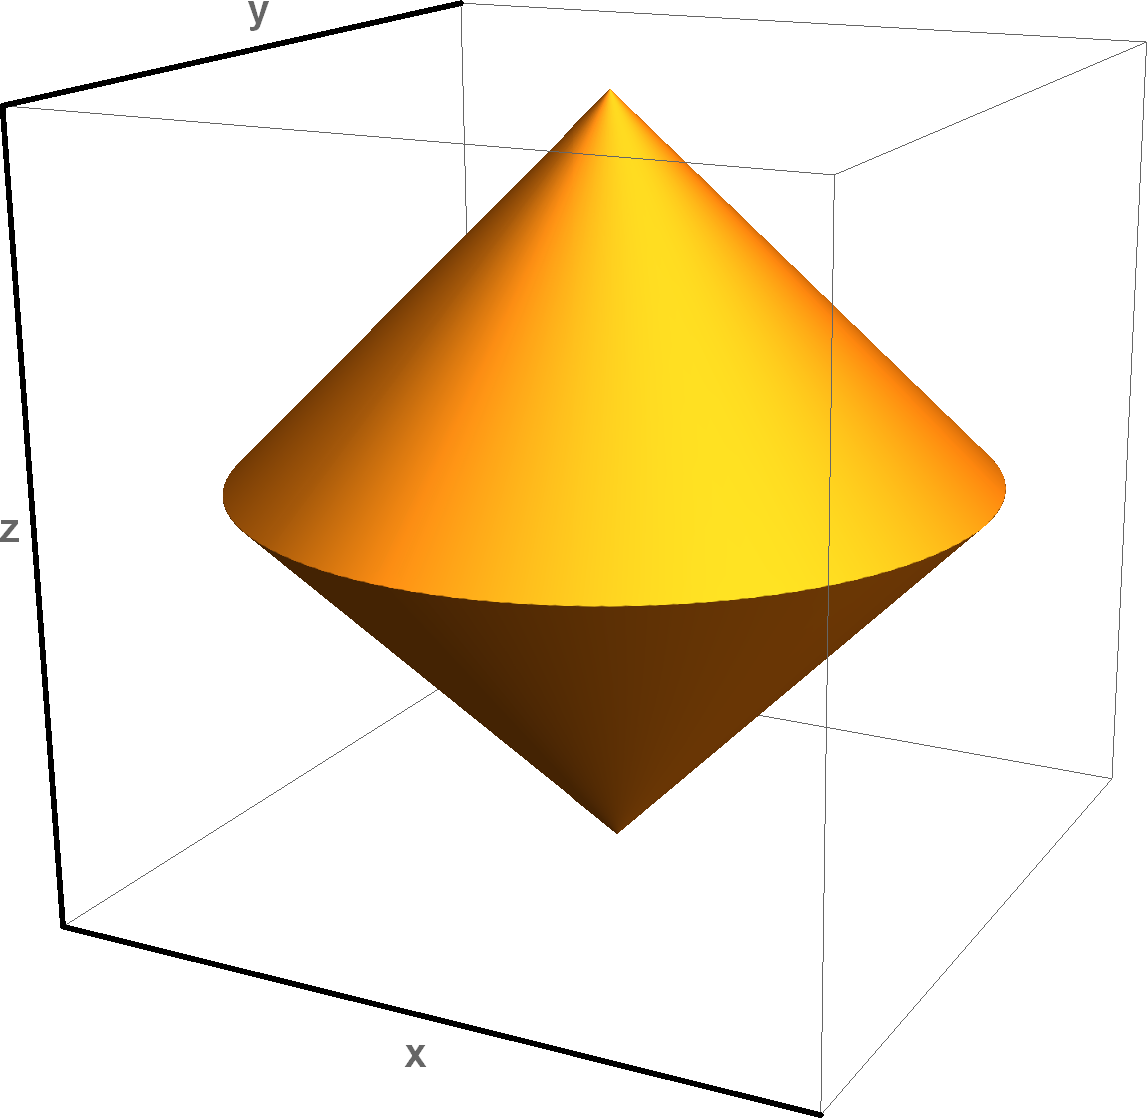
\includegraphics[width=0.2\textwidth]{../images/form_factor/supershapes/superquadric111_1_2.png}
    & 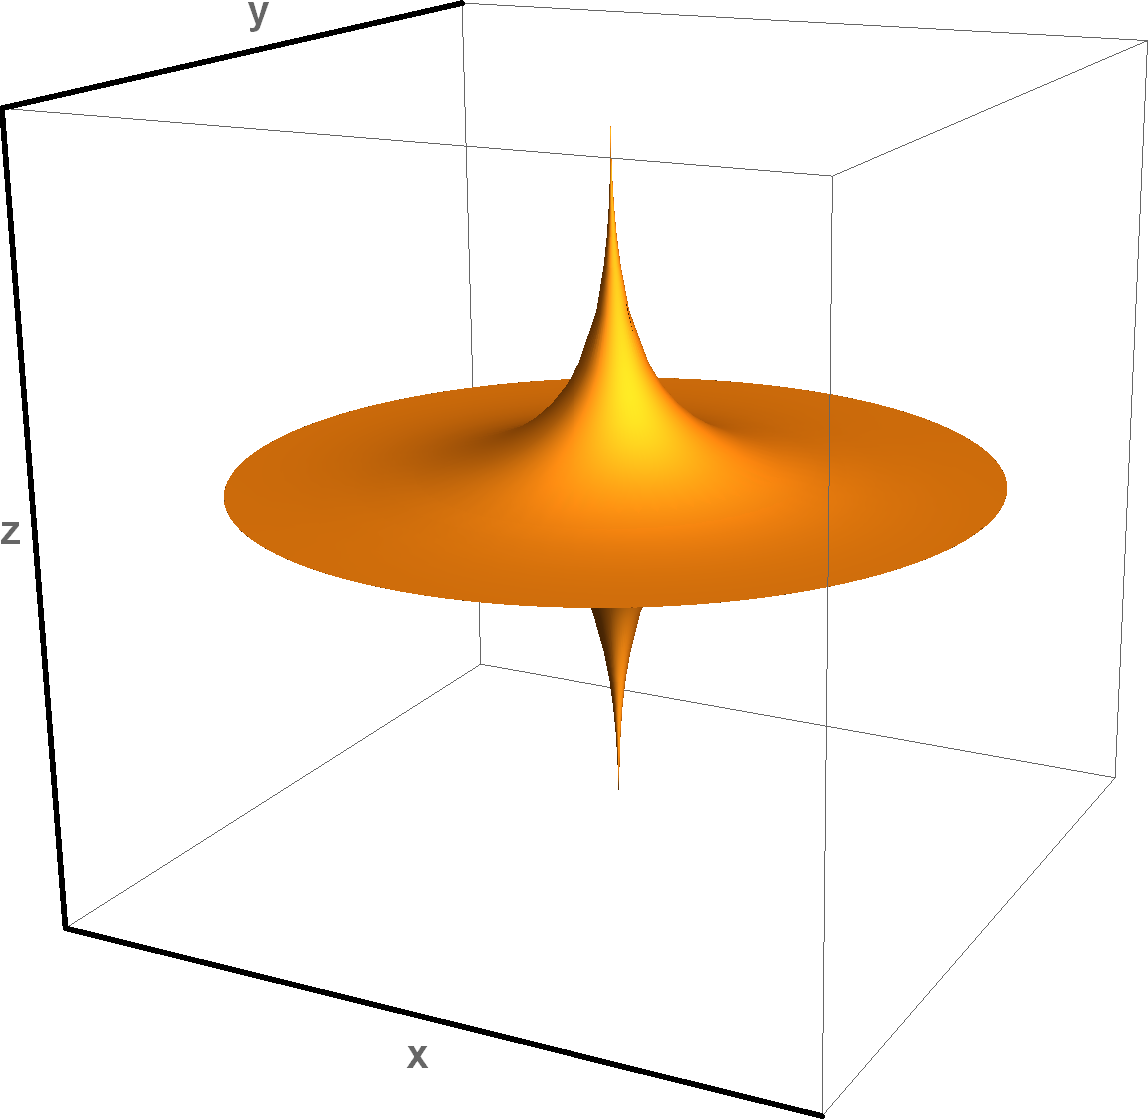
\includegraphics[width=0.2\textwidth]{../images/form_factor/supershapes/superquadric111_1_5.png} \\
  $\epsilon_1=2$
    & 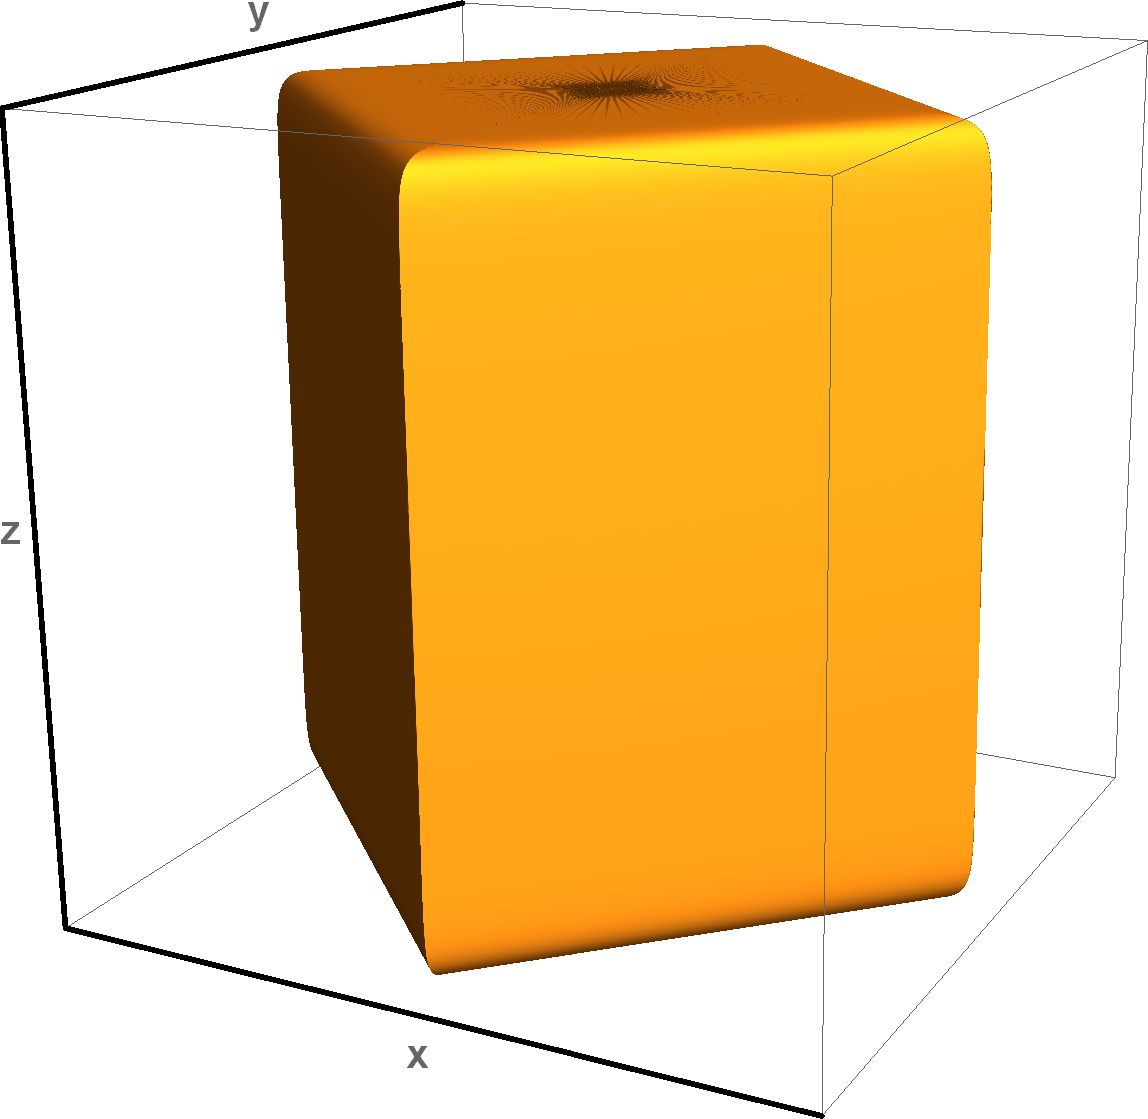
\includegraphics[width=0.2\textwidth]{../images/form_factor/supershapes/superquadric111_2_01.png}
    & 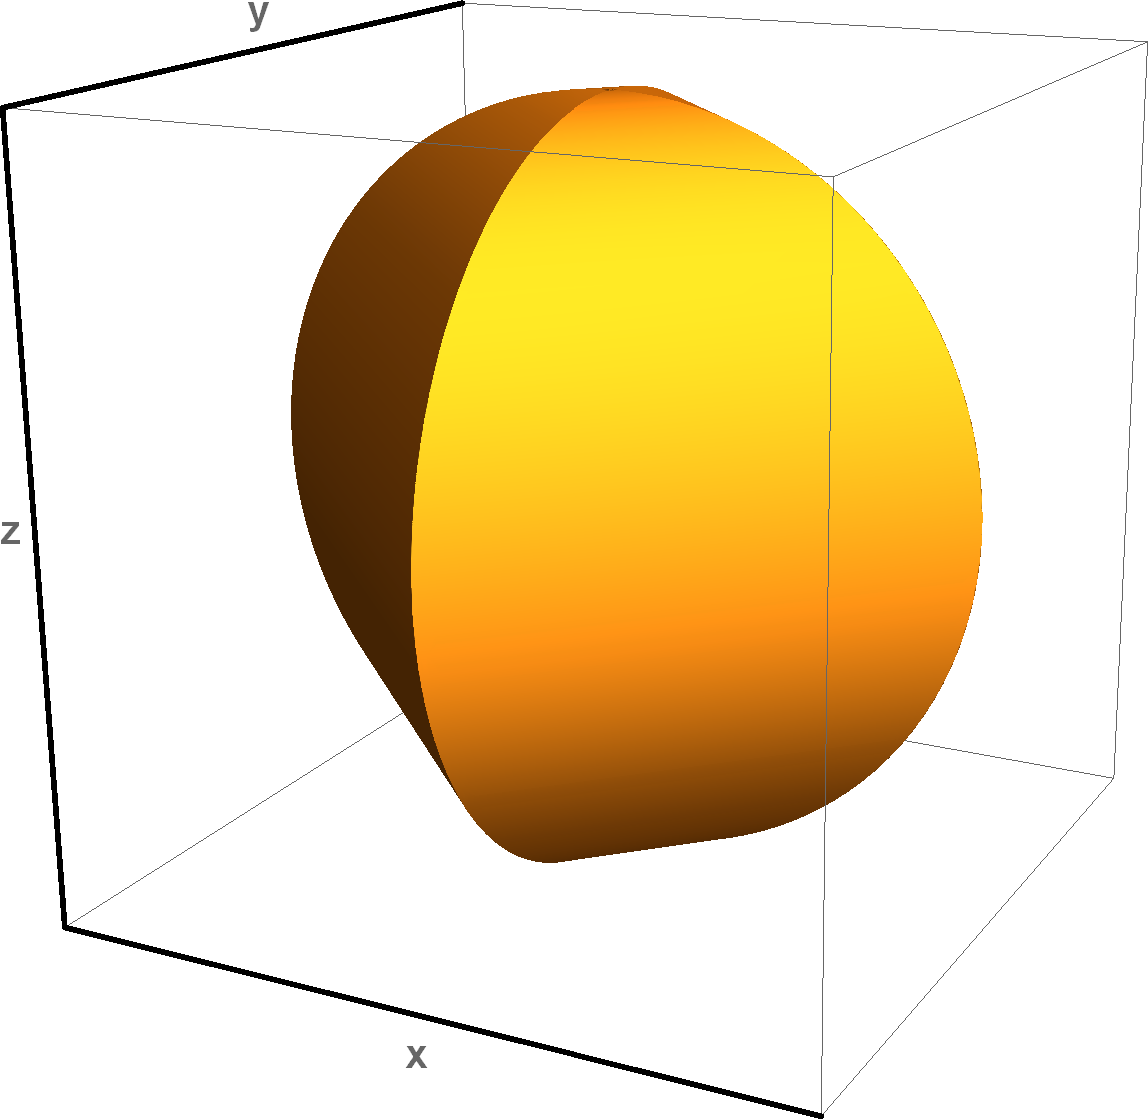
\includegraphics[width=0.2\textwidth]{../images/form_factor/supershapes/superquadric111_2_1.png}
    & 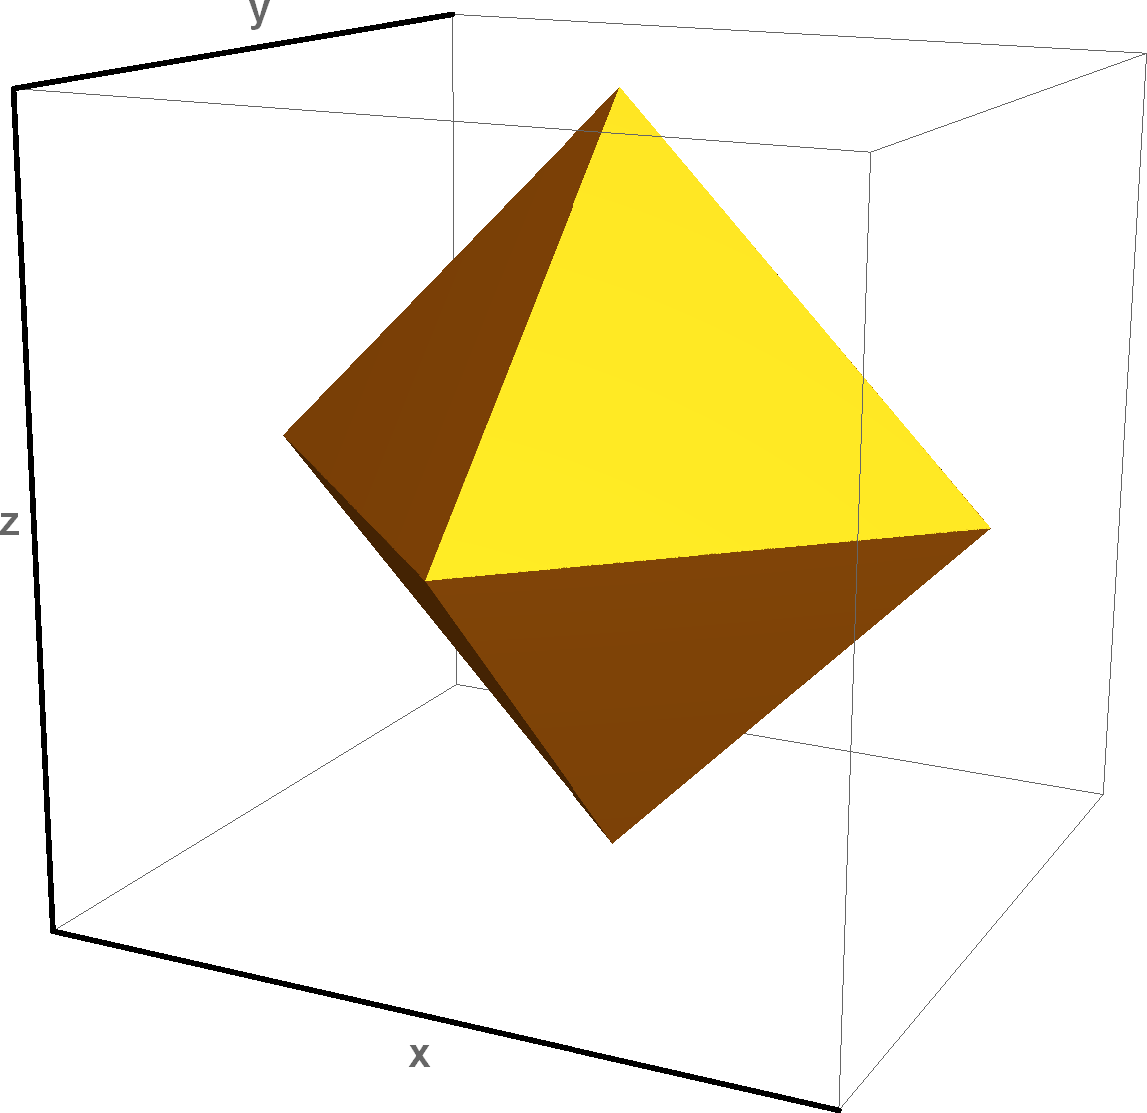
\includegraphics[width=0.2\textwidth]{../images/form_factor/supershapes/superquadric111_2_2.png}
    & 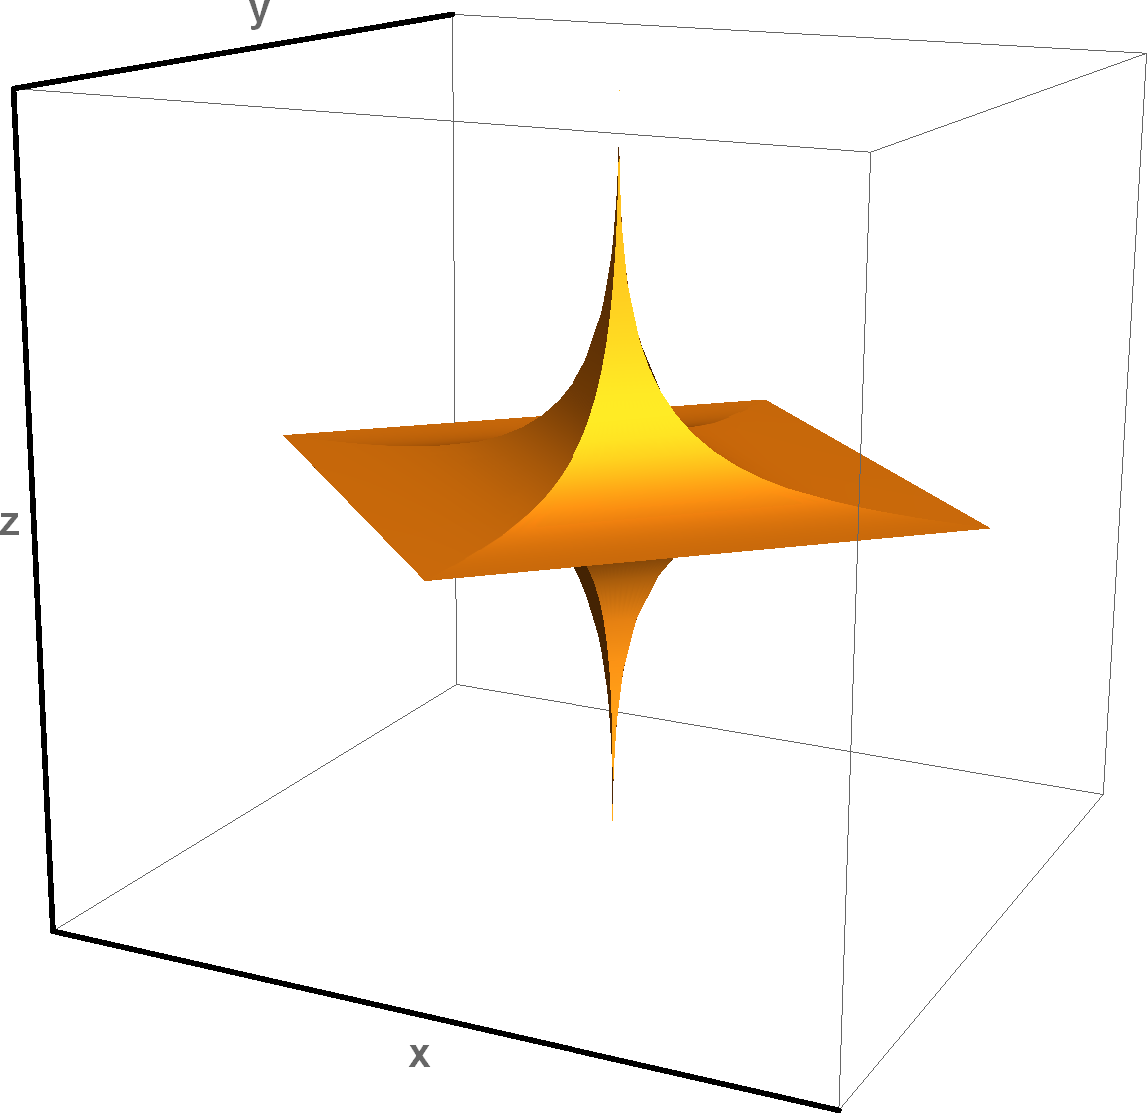
\includegraphics[width=0.2\textwidth]{../images/form_factor/supershapes/superquadric111_2_5.png} \\
  $\epsilon_1=5$
    & 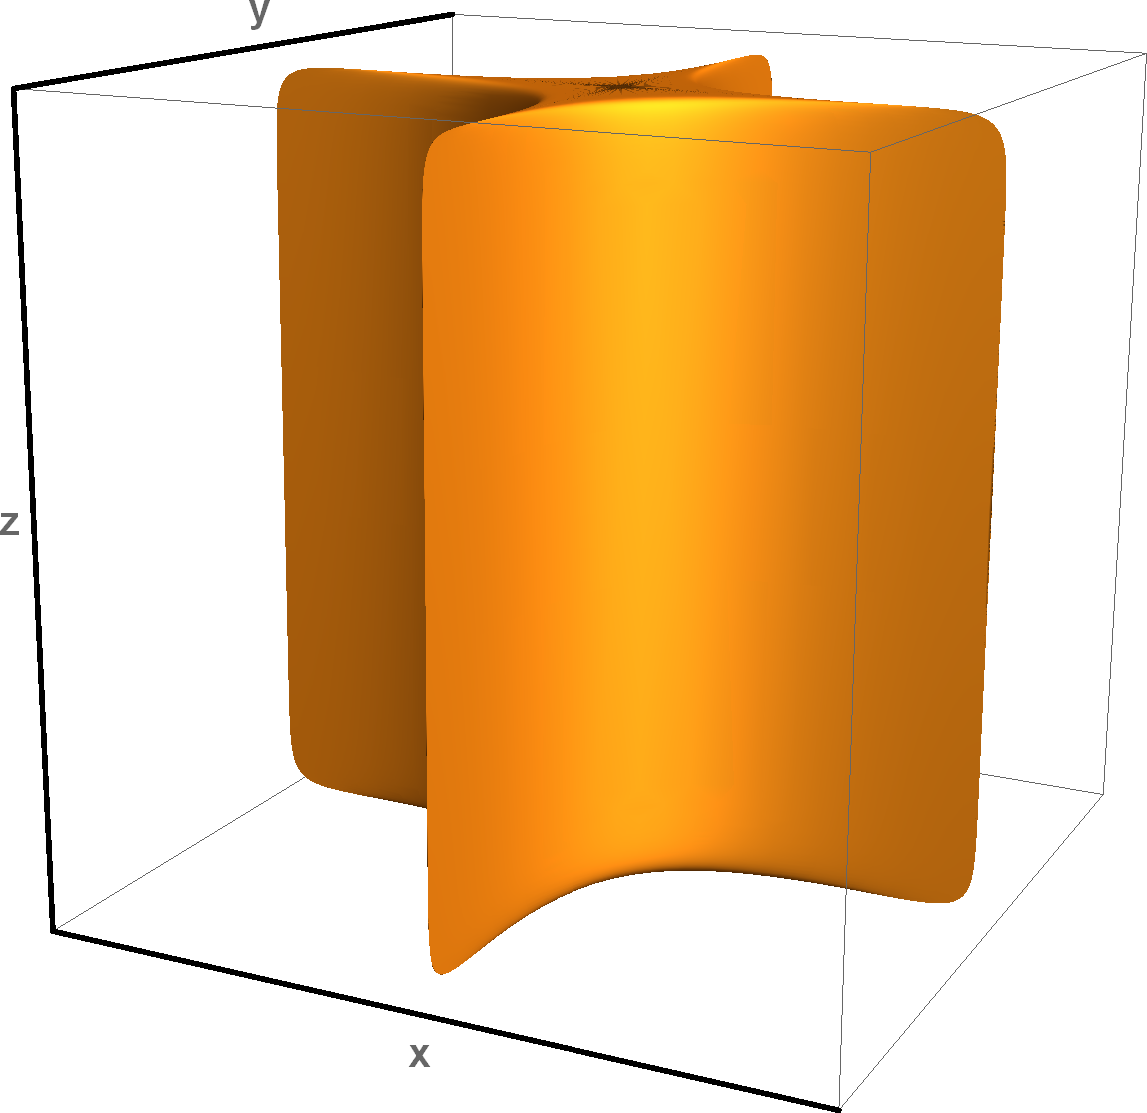
\includegraphics[width=0.2\textwidth]{../images/form_factor/supershapes/superquadric111_5_01.png}
    & 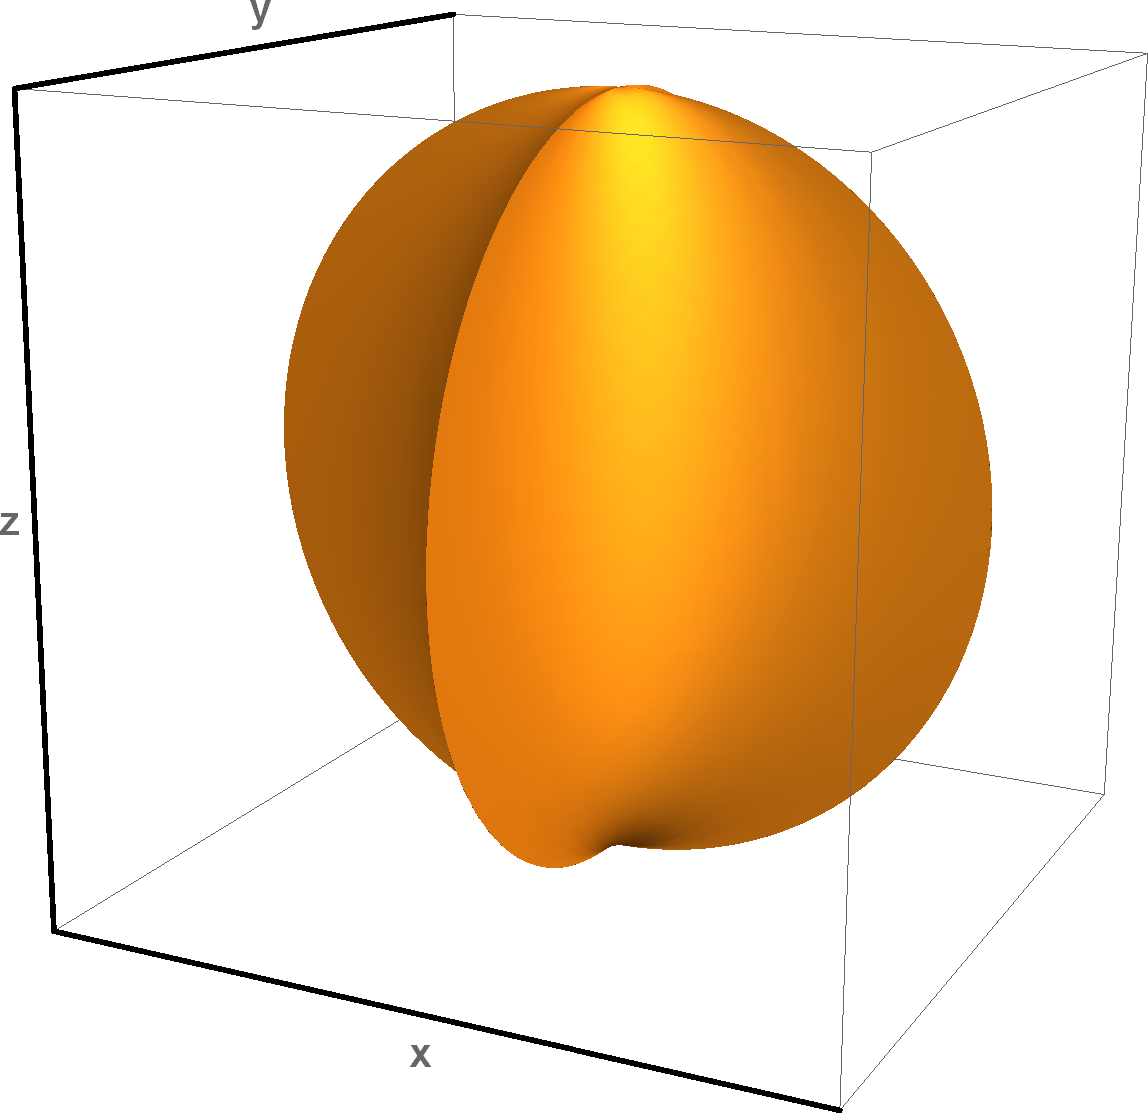
\includegraphics[width=0.2\textwidth]{../images/form_factor/supershapes/superquadric111_5_1.png}
    & 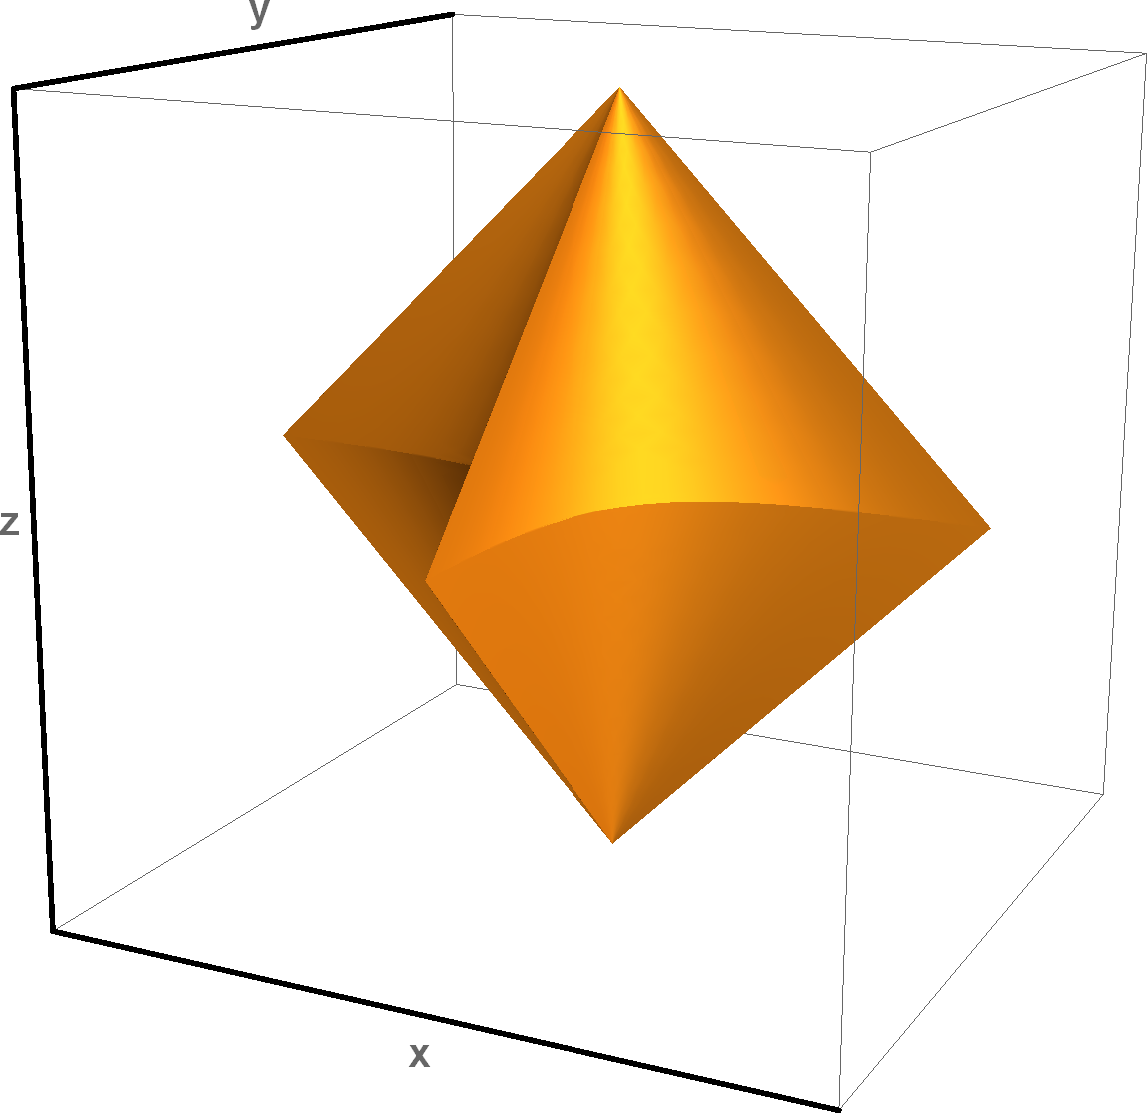
\includegraphics[width=0.2\textwidth]{../images/form_factor/supershapes/superquadric111_5_2.png}
    & 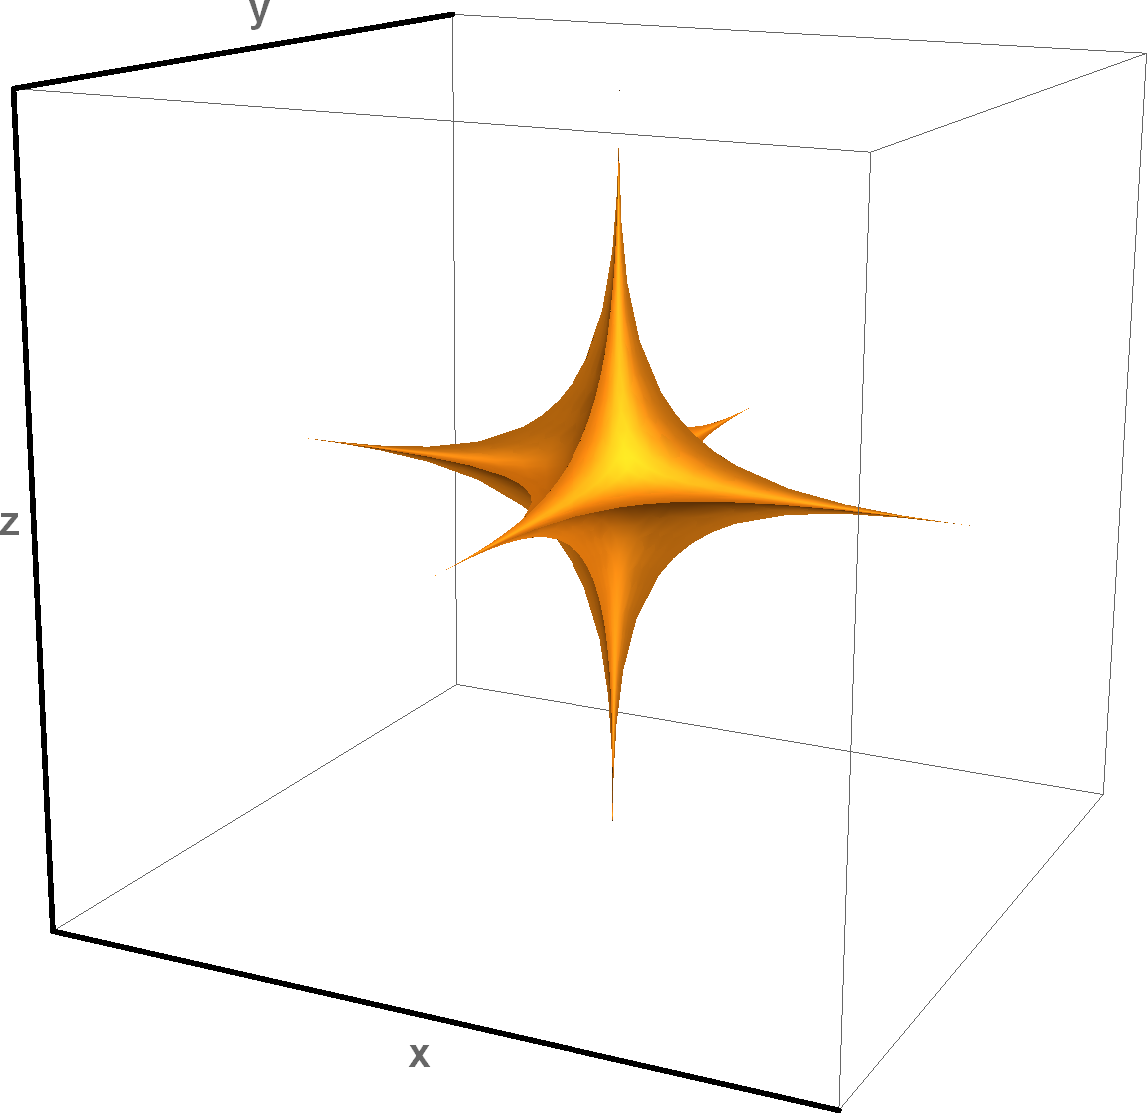
\includegraphics[width=0.2\textwidth]{../images/form_factor/supershapes/superquadric111_5_5.png} \\
  & $\epsilon_2=0.1$ & $\epsilon_2=1$ & $\epsilon_2=2$ & $\epsilon_2=5$
\end{tabular}
\caption{Typical superquadrics. The parameters for scale factors are $a_1 = a_2 = a_3 = 1 $. The values for $\epsilon_2$ vary horizontally by $\epsilon_2=0.1, 1,2,5$ and vertically by $\epsilon_1=0.1, 1,2,5$.}
\label{fig:opo_superquadrics}
\end{figure}

Super-quadrics have been widely used in computer graphics \cite{Barr1981}. They have both a
parametric and an implicit representation. The parametric representation of the surface is defined by
\begin{align}\label{eq:superquadrics:parametric}
  \left(
    \begin{array}{c}
      x(a_1\theta,\phi) \\
      y(a_2\theta,\phi) \\
      z(a_3\theta,\phi) \\
    \end{array}
  \right)
 &=
 \left(
    \begin{array}{c}
     a_1 \operatorname{sgnpow}(\cos\theta,\epsilon_2)\operatorname{sgnpow}(\cos\phi,\epsilon_1)  \\
     a_2 \operatorname{sgnpow}(\sin\theta,\epsilon_2)\operatorname{sgnpow}(\cos\phi,\epsilon_1)  \\
     a_3 \operatorname{sgnpow}(\sin\phi,\epsilon_1) \\
    \end{array}
  \right)
\end{align}
whereas the signed power function is defined as
\begin{align}\label{eq:sgnpow}
  \operatorname{sgnpow}(t,\epsilon) &= \operatorname{sgn}(t)\abs{t}^\epsilon \\
  \operatorname{sgn}(t) &=
  \begin{cases}
    -1&{\text{if }}x<0,\\
     0&{\text{if }}x=0,\\
     1&{\text{if }}x>0.
  \end{cases}
\end{align}
The implicit representation is given by
\begin{align}\label{eq:superquadrics:implicit}
\left(
     \left(\frac{x}{a_1}\right)^{\frac{2}{\epsilon_2}}+
     \left(\frac{y}{a_2}\right)^{\frac{2}{\epsilon_2}}
\right)^{\frac{\epsilon_2}{\epsilon_1}} +
\left(\frac{z}{a_3}\right)^{\frac{2}{\epsilon_1}} &\leq 1
\end{align}
Super-ellipsoids are a special case of super-quadrics for which the two exponents are equal $\epsilon_1=\epsilon_2$. The implicit representation then looks as
$\abs{\frac{x}{a_1}}^n+\abs{\frac{y}{a_2}}^n+\abs{\frac{y}{a_3}}^n\leq 1$ with $n=1/\epsilon_1=1/\epsilon_2$.
As the asymmetric super-quadrics is obtained by a scale transform, which is a special case of an affine transform only the Fourier transform of a unit super-quadrics has to be solved. All its affine transform than can be easily calculated by linear algebra.  The Fourier transform of a unit super-quadrics ($a_1=a_2=a_3=1$) is
\begin{align}\label{eq:FTsuperquadrics}
  F_\mathrm{SQ}(\B{Q}) &=
\det(\M{D}^{-1})\, e^{-\imath\B{QR}}\, \Delta\eta\, \int\limits_{-1}^1
\mathrm{d}x\, \int\limits_{-Y(x)}^{Y(x)} \mathrm{d}y\,  \int\limits_{-Z(x,y)}^{Z(x,y)} \mathrm{d}z \,
e^{\imath\B{\hat{Q}r}} \nonumber \\
 &=
\det(\M{D}^{-1})\, e^{-\imath\B{QR}}\, \Delta\eta\,   \\
& \times \int\limits_{-1}^1
\mathrm{d}x\, \int\limits_{-Y(x)}^{Y(x)} \mathrm{d}y\,
e^{\imath\left(\hat{Q}_xx+\hat{Q}_yy\right)} 2Z(x,y)\operatorname{sinc}(\hat{Q}_z Z(x,y))\nonumber \\
&= \det(\M{D}^{-1})\, e^{-\imath\B{QR}}\, \Delta\eta\, \\
& \times \int\limits_{-1}^1
\mathrm{d}x\, \int\limits_{-1}^{1} \mathrm{d}s\,
e^{\imath\left(\hat{Q}_xx+\hat{Q}_yY(x)s\right)} 2Z(x,Y(x)s)\operatorname{sinc}(\hat{Q}_z Z(x,Y(x)s))Y(x)\nonumber \\
Y(x) &= \left(1-x^{\frac{2}{\epsilon_2}}\right)^{\frac{\epsilon_2}{2}}\\
Z(x,y) &= \left(1-\left(x^{\frac{2}{\epsilon_2}}+y^{\frac{2}{\epsilon_2}}\right)^{\frac{\epsilon_2}{\epsilon_1}}\right)^{\frac{\epsilon_1}{2}}
\end{align}
To make use of numerical integration routines for multiple dimensions over hypercubes it might be convenient to perform a variable transformation using $ x(r,\theta,\phi)$ and $ y(r,\theta,\phi)$ given in eq.\ \ref{eq:superquadrics:parametric}. The Jacobi determinant for this substitution is
\begin{align}\label{eq:detJ_superquadrics}
  \det{\M{J}} &= \det
  \left(
    \begin{array}{cc}
      \frac{\partial x(r,\theta,0)}{\partial r}      & \frac{\partial y(r,\theta,0)}{\partial r}\\
      \frac{\partial x(r,\theta,0)}{\partial \theta} & \frac{\partial y(r,\theta,0)}{\partial \theta}
    \end{array}
  \right) = \epsilon_2 r \abs{\cos\theta\sin\theta}^{\epsilon_2-1}
\end{align}
so that
\begin{align}
\begin{split}
F_\mathrm{SQ}(\B{Q}) &= 8 \det(\M{D}^{-1})\, e^{-\imath\B{QR}}\, \Delta\eta\,\int\limits_{0}^1
\mathrm{d}r\, \int\limits_{0}^{\pi/2} \mathrm{d}\theta\,  \epsilon_2 r \abs{\cos\theta\sin\theta}^{\epsilon_2-1}\\
     &\times \cos\left(\hat{Q}_xx(r,\theta,0)+\hat{Q}_yy(r,\theta,0)\right) Z\operatorname{sinc}(\hat{Q}_z Z)\nonumber \\
Z &= \left(1-\left(x(r,\theta,0)^{\frac{2}{\epsilon_2}}+y(r,\theta,0)^{\frac{2}{\epsilon_2}}\right)^{\frac{\epsilon_2}{\epsilon_1}}\right)^{\frac{\epsilon_1}{2}}
\end{split}
\end{align}

\begin{figure}[thb]
\begingroup
\setlength{\tabcolsep}{1pt}
\def\arraystretch{0.4}%
 \captionsetup[subfigure]{position=b}
\centering
\subcaptionbox{$(\epsilon_1,\epsilon_2)=(1,2)$ \label{fig:superquadricsIQ2D_1}}{
\begin{tabular}{llll}
%\toprule  \\ %\midrule
2m   & 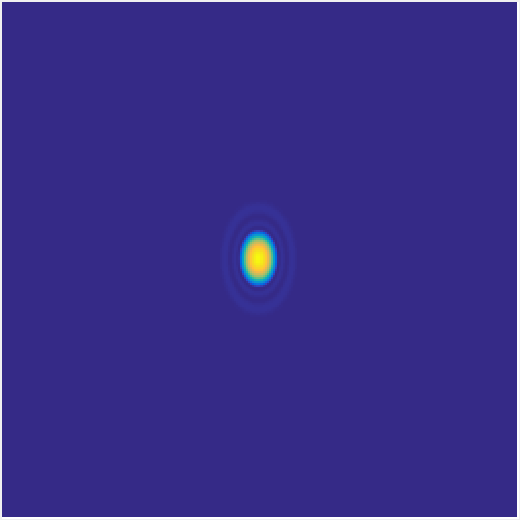
\includegraphics[width=0.13\textwidth]{../images/form_factor/supershapes/superquadrics_1_2_0_0_0_2m.png}
     & 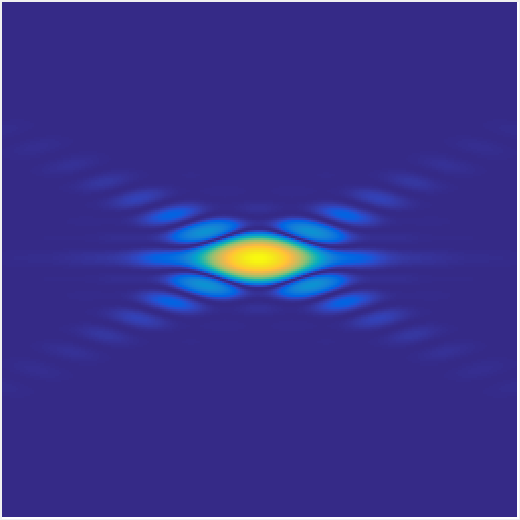
\includegraphics[width=0.13\textwidth]{../images/form_factor/supershapes/superquadrics_1_2_0_90_0_2m.png}
     & \includegraphics[width=0.13\textwidth]{../images/form_factor/supershapes/superquadrics_1_2_0_45_45_2m.png}  \\
6m   & \includegraphics[width=0.13\textwidth]{../images/form_factor/supershapes/superquadrics_1_2_0_0_0_6m.png}
     & \includegraphics[width=0.13\textwidth]{../images/form_factor/supershapes/superquadrics_1_2_0_90_0_6m.png}
     & \includegraphics[width=0.13\textwidth]{../images/form_factor/supershapes/superquadrics_1_2_0_45_45_6m.png}  \\
18m  & \includegraphics[width=0.13\textwidth]{../images/form_factor/supershapes/superquadrics_1_2_0_0_0_18m.png}
     & \includegraphics[width=0.13\textwidth]{../images/form_factor/supershapes/superquadrics_1_2_0_90_0_18m.png}
     & \includegraphics[width=0.13\textwidth]{../images/form_factor/supershapes/superquadrics_1_2_0_45_45_18m.png}  \\
%\diagbox{sampl.-det.}{$(\alpha,\beta,\gamma)$}
     & {\small $(0^\circ,0^\circ,0^\circ)$}
     & {\small $(0^\circ,90^\circ,0^\circ)$}
     & {\small $(0^\circ,45^\circ,45^\circ)$}  %\bottomrule
\end{tabular}
}
\hfill
\subcaptionbox{$(\epsilon_1,\epsilon_2)=(2,0.1)$ \label{fig:superquadricsIQ2D_2}}{
\begin{tabular}{llll}
%\toprule
2m   & \includegraphics[width=0.13\textwidth]{../images/form_factor/supershapes/superquadrics_2_01_0_0_0_2m.png}
     & \includegraphics[width=0.13\textwidth]{../images/form_factor/supershapes/superquadrics_2_01_0_90_0_2m.png}
     & \includegraphics[width=0.13\textwidth]{../images/form_factor/supershapes/superquadrics_2_01_0_45_45_2m.png}  \\
6m   & \includegraphics[width=0.13\textwidth]{../images/form_factor/supershapes/superquadrics_2_01_0_0_0_6m.png}
     & \includegraphics[width=0.13\textwidth]{../images/form_factor/supershapes/superquadrics_2_01_0_90_0_6m.png}
     & \includegraphics[width=0.13\textwidth]{../images/form_factor/supershapes/superquadrics_2_01_0_45_45_6m.png}  \\
18m  & \includegraphics[width=0.13\textwidth]{../images/form_factor/supershapes/superquadrics_2_01_0_0_0_18m.png}
     & \includegraphics[width=0.13\textwidth]{../images/form_factor/supershapes/superquadrics_2_01_0_90_0_18m.png}
     & \includegraphics[width=0.13\textwidth]{../images/form_factor/supershapes/superquadrics_2_01_0_45_45_18m.png}  \\
%\diagbox{sampl.-det.}{$(\alpha,\beta,\gamma)$}
     & {\small $(0^\circ,0^\circ,0^\circ)$}
     & {\small $(0^\circ,90^\circ,0^\circ)$}
     & {\small $(0^\circ,45^\circ,45^\circ)$}  %\bottomrule
\end{tabular}
}

\vspace{5mm}

\subcaptionbox{$(\epsilon_1,\epsilon_2)=(1,2)$ \label{fig:superquadricsIQ2D_3}}{
\begin{tabular}{llll}
%\toprule
2m   & \includegraphics[width=0.13\textwidth]{../images/form_factor/supershapes/superquadrics_2_2_0_0_0_2m.png}
     & \includegraphics[width=0.13\textwidth]{../images/form_factor/supershapes/superquadrics_2_2_0_90_0_2m.png}
     & \includegraphics[width=0.13\textwidth]{../images/form_factor/supershapes/superquadrics_2_2_0_45_45_2m.png}  \\
6m   & \includegraphics[width=0.13\textwidth]{../images/form_factor/supershapes/superquadrics_2_2_0_0_0_6m.png}
     & \includegraphics[width=0.13\textwidth]{../images/form_factor/supershapes/superquadrics_2_2_0_90_0_6m.png}
     & \includegraphics[width=0.13\textwidth]{../images/form_factor/supershapes/superquadrics_2_2_0_45_45_6m.png}  \\
18m  & \includegraphics[width=0.13\textwidth]{../images/form_factor/supershapes/superquadrics_2_2_0_0_0_18m.png}
     & \includegraphics[width=0.13\textwidth]{../images/form_factor/supershapes/superquadrics_2_2_0_90_0_18m.png}
     & \includegraphics[width=0.13\textwidth]{../images/form_factor/supershapes/superquadrics_2_2_0_45_45_18m.png}  \\
%\diagbox{sampl.-det.}{$(\alpha,\beta,\gamma)$}
     & {\small $(0^\circ,0^\circ,0^\circ)$}
     & {\small $(0^\circ,90^\circ,0^\circ)$}
     & {\small $(0^\circ,45^\circ,45^\circ)$}  %\bottomrule
\end{tabular}
}
\hfill
\subcaptionbox{$(\epsilon_1,\epsilon_2)=(2,0.1)$ \label{fig:superquadricsIQ2D_4}}{
\begin{tabular}{llll}
%\toprule
2m   & \includegraphics[width=0.13\textwidth]{../images/form_factor/supershapes/superquadrics_2_5_0_0_0_2m.png}
     & \includegraphics[width=0.13\textwidth]{../images/form_factor/supershapes/superquadrics_2_5_0_90_0_2m.png}
     & \includegraphics[width=0.13\textwidth]{../images/form_factor/supershapes/superquadrics_2_5_0_45_45_2m.png}  \\
6m   & \includegraphics[width=0.13\textwidth]{../images/form_factor/supershapes/superquadrics_2_5_0_0_0_6m.png}
     & \includegraphics[width=0.13\textwidth]{../images/form_factor/supershapes/superquadrics_2_5_0_90_0_6m.png}
     & \includegraphics[width=0.13\textwidth]{../images/form_factor/supershapes/superquadrics_2_5_0_45_45_6m.png}  \\
18m  & \includegraphics[width=0.13\textwidth]{../images/form_factor/supershapes/superquadrics_2_5_0_0_0_18m.png}
     & \includegraphics[width=0.13\textwidth]{../images/form_factor/supershapes/superquadrics_2_5_0_90_0_18m.png}
     & \includegraphics[width=0.13\textwidth]{../images/form_factor/supershapes/superquadrics_2_5_0_45_45_18m.png}  \\
%\diagbox{sampl.-det.}{$(\alpha,\beta,\gamma)$}
     & {\small $(0^\circ,0^\circ,0^\circ)$}
     & {\small $(0^\circ,90^\circ,0^\circ)$}
     & {\small $(0^\circ,45^\circ,45^\circ)$}  %\bottomrule
\end{tabular}
}
\endgroup
  \caption{Scattering patterns for super-quadrics with scale factors are $a_1=30$nm, $a_2=20$nm, $a_3=10$nm calculated for detector distances (2m, 6m, 18m) and a wavelength of 0.6nm are shown. Three orientation using Tait–Bryan angles (yaw-
pitch-roll) are shown.} \label{fig:superquadricsIQ2D}
\end{figure}

\clearpage
\subsection{oriented super-egg} ~\\

\begin{figure}[htb]
\begin{tabular}{ccccc}
     \includegraphics[width=0.18\textwidth]{../images/form_factor/supershapes/SuperEggPietHein.png}
    & \includegraphics[width=0.18\textwidth]{../images/form_factor/supershapes/SuperEgg08.png}
    & \includegraphics[width=0.18\textwidth]{../images/form_factor/supershapes/SuperEgg1.png}
    & \includegraphics[width=0.18\textwidth]{../images/form_factor/supershapes/SuperEgg2.png}
    & \includegraphics[width=0.18\textwidth]{../images/form_factor/supershapes/SuperEgg5.png} \\
     $\epsilon_1=0.4$ & $\epsilon_1=0.8$ & $\epsilon_1=1$ & $\epsilon_1=2$ & $\epsilon_1=5$
\end{tabular}
\caption{Supereggs. The parameters for the scale factors of the shown supereggs are $a_1 = a_2 = a_3 = 4/3$. The values for $\epsilon_2=2$ and $\epsilon_1=0.4, 0.8, 1,2,5$.}
\label{fig:opo_superegg}
\end{figure}

The superegg is a super-quadrics whose horizontal cross-sections are ellipses, i.e. $\epsilon_2=1$. It is defined by the inequality \cite{WeisssteinSuperEgg}
\begin{align}
\label{eq:superegg_implicit}
   \left(\sqrt{\left(\frac{x}{a_1}\right)^2+\left(\frac{y}{a_2}\right)^2}\right)^{\frac{2}{\epsilon1}} + \left(\frac{z}{a_3}\right)^{\frac{2}{\epsilon1}} & \leq 1
\end{align}
For circular cross-sections the Fourier transform \cite{Maric2017} can be written as a single integral. For the more general case of an elliptical cross-section the Fourier transform still can be written as a single integral, however, the orientation average becomes a double integral as the cylinder symmetry get lost.
\begin{align}
F_\mathrm{SEgg}(\B{Q}) &=
\det(\M{D}^{-1})\, e^{-\imath\B{QR}}\, \Delta\eta\,  \nonumber \\
 &\times \int_0^1 \frac{4 \pi  r \sin \left(\hat{Q}_z \left(1-r^{2/\epsilon_1}\right)^{\epsilon_1/2}\right) \operatorname{J}_0\left(\sqrt{\hat{Q}_x^2+\hat{Q}_y^2}
   r\right)}{\hat{Q}_z} \mathrm{d}r
\end{align}

\clearpage
\subsection{oriented super-shapes and rational super-shaped} ~\\
\begin{figure}[htb]
\begingroup
\setlength{\tabcolsep}{1pt}
\def\arraystretch{0.4}%
\begin{tabular}{ccccccccc}
    & \includegraphics[width=0.12\textwidth]{../images/form_factor/supershapes/SuperShape3D5_0_30_20_20_1_1__7_0p38_75_20_20_1_1.png}
    & \includegraphics[width=0.12\textwidth]{../images/form_factor/supershapes/SuperShape3D6_0_100_40_40_1_1__8_0p4_200_40_40_1_1__a1b1c1p5.png}
    & \includegraphics[width=0.12\textwidth]{../images/form_factor/supershapes/SuperShape3D1p5_0_2_12_12_1_1__4_0_2_2_2_1_1__a3b1c3.png}
    & \includegraphics[width=0.12\textwidth]{../images/form_factor/supershapes/SuperShape3D3_0_1_6_6_1_1__4_0_2_2_2_1_1.png}
    & \includegraphics[width=0.12\textwidth]{../images/form_factor/supershapes/SuperShape3D5_0_1_6_6_1_1__4_0_2_2_2_1_1.png}
    & \includegraphics[width=0.12\textwidth]{../images/form_factor/supershapes/SuperShape3D7p3_0_5_5_5_5_1__4_0_5_5_5_6_2.png}
    & \includegraphics[width=0.12\textwidth]{../images/form_factor/supershapes/SuperShape3D4_0_2_2_2_1_1__24_0_2_8_8_1_1__a1b1c1.png}
    & \includegraphics[width=0.12\textwidth]{../images/form_factor/supershapes/SuperShape3D4_0_2_2_2_1_1__24_0_2_8_8_1_1__a1b1c1_gamma90.png} \\
6m    & \includegraphics[width=0.12\textwidth]{../images/form_factor/supershapes/SuperShapeIQ5_0_30_20_20_1_1__7_0p38_75_20_20_1_1_6m.png}
    & \includegraphics[width=0.12\textwidth]{../images/form_factor/supershapes/SuperShapeIQ6_0_100_40_40_1_1__8_0p4_200_40_40_1_1__a1b1c1p5_6m.png}
    & \includegraphics[width=0.12\textwidth]{../images/form_factor/supershapes/SuperShapeIQ1p5_0_2_12_12_1_1__4_0_2_2_2_1_1__a3b1c3_6m.png}
    & \includegraphics[width=0.12\textwidth]{../images/form_factor/supershapes/SuperShapeIQ3_0_1_6_6_1_1__4_0_2_2_2_1_1_6m.png}
    & \includegraphics[width=0.12\textwidth]{../images/form_factor/supershapes/SuperShapeIQ5_0_1_6_6_1_1__4_0_2_2_2_1_1_6m.png}
    & \includegraphics[width=0.12\textwidth]{../images/form_factor/supershapes/SuperShapeIQ7p3_0_5_5_5_5_1__4_0_5_5_5_6_2_a1b1c1_6m.png}
    & \includegraphics[width=0.12\textwidth]{../images/form_factor/supershapes/SuperShapeIQ4_0_2_2_2_1_1__24_0_2_8_8_1_1__a1b1c1_gamma0_6m.png}
    & \includegraphics[width=0.12\textwidth]{../images/form_factor/supershapes/SuperShapeIQ4_0_2_2_2_1_1__24_0_2_8_8_1_1__a1b1c1_gamma90_6m.png}\\
 18m   & \includegraphics[width=0.12\textwidth]{../images/form_factor/supershapes/SuperShapeIQ5_0_30_20_20_1_1__7_0p38_75_20_20_1_1_18m.png}
    & \includegraphics[width=0.12\textwidth]{../images/form_factor/supershapes/SuperShapeIQ6_0_100_40_40_1_1__8_0p4_200_40_40_1_1__a1b1c1p5_18m.png}
    & \includegraphics[width=0.12\textwidth]{../images/form_factor/supershapes/SuperShapeIQ1p5_0_2_12_12_1_1__4_0_2_2_2_1_1__a3b1c3_18m.png}
    & \includegraphics[width=0.12\textwidth]{../images/form_factor/supershapes/SuperShapeIQ3_0_1_6_6_1_1__4_0_2_2_2_1_1_18m.png}
    & \includegraphics[width=0.12\textwidth]{../images/form_factor/supershapes/SuperShapeIQ5_0_1_6_6_1_1__4_0_2_2_2_1_1_18m.png}
    & \includegraphics[width=0.12\textwidth]{../images/form_factor/supershapes/SuperShapeIQ7p3_0_5_5_5_5_1__4_0_5_5_5_6_2_a1b1c1_18m.png}
    & \includegraphics[width=0.12\textwidth]{../images/form_factor/supershapes/SuperShapeIQ4_0_2_2_2_1_1__24_0_2_8_8_1_1__a1b1c1_gamma0_18m.png}
    & \includegraphics[width=0.12\textwidth]{../images/form_factor/supershapes/SuperShapeIQ4_0_2_2_2_1_1__24_0_2_8_8_1_1__a1b1c1_gamma90_18m.png} \\
    & {\small \footnotesize \scriptsize \tiny \begin{tabular}{l}
         $m=5,7$ \\
         $\alpha=0,0.38$ \\
         $a=1,1$\\
         $b=1,1$ \\
         $n_1=30,75$\\
         $n_2=20,20$\\
         $n_3=20,20$ \\
         $a_1=30$nm \\
         $a_2=30$nm \\
         $a_3=30$nm \\ $\gamma=0^\circ$
       \end{tabular}  }
    &  {\small \footnotesize \scriptsize \tiny \begin{tabular}{l}
         $m=6,8$ \\
         $\alpha=0,0.4$ \\
         $a=1,1$\\
         $b=1,1$ \\
         $n_1=100,200$\\
         $n_2=40,40$\\
         $n_3=40,40$ \\
         $a_1=30$nm \\
         $a_2=30$nm\\
         $a_3=45$nm \\ $\gamma=0^\circ$
       \end{tabular}  }
    &  {\small \footnotesize \scriptsize \tiny \begin{tabular}{l}
         $m=1.5,4$ \\
         $\alpha=0,0$ \\
         $a=1,1$\\
         $b=1,1$ \\
         $n_1=2,2$\\
         $n_2=12,2$\\
         $n_3=12,2$ \\
         $a_1=30$nm \\
         $a_2=10$nm\\
         $a_3=30$nm \\ $\gamma=0^\circ$
       \end{tabular}  }
    & {\small \footnotesize \scriptsize \tiny \begin{tabular}{l}
         $m=3,4$ \\
         $\alpha=0,0$ \\
         $a=1,1$\\
         $b=1,1$ \\
         $n_1=1,2$\\
         $n_2=6,2$\\
         $n_3=6,2$ \\
         $a_1=30$nm \\
         $a_2=30$nm \\
         $a_3=30$nm \\ $\gamma=0^\circ$
       \end{tabular}  }
    & {\small \footnotesize \scriptsize \tiny \begin{tabular}{l}
         $m=5,4$ \\
         $\alpha=0,0$ \\
         $a=1,1$\\
         $b=1,1$ \\
         $n_1=1,2$\\
         $n_2=6,2$\\
         $n_3=6,2$ \\
         $a_1=30$nm \\
         $a_2=30$nm \\
         $a_3=30$nm \\ $\gamma=0^\circ$
       \end{tabular}  }
    & {\small \footnotesize \scriptsize \tiny \begin{tabular}{l}
         $m=7.3,4$ \\
         $\alpha=0,0$ \\
         $a=5,6$\\
         $b=1,2$ \\
         $n_1=5,5$\\
         $n_2=5,5$\\
         $n_3=5,5$ \\
         $a_1=30$nm \\
         $a_2=30$nm \\
         $a_3=30$nm \\ $\gamma=0^\circ$
       \end{tabular}  }
    & {\small \footnotesize \scriptsize \tiny \begin{tabular}{l}
         $m=4,24$ \\
         $\alpha=0,0$ \\
         $a=1,1$\\
         $b=1,1$ \\
         $n_1=2,2$\\
         $n_2=2,8$\\
         $n_3=2,8$ \\
         $a_1=30$nm \\
         $a_2=30$nm \\
         $a_3=30$nm \\ $\gamma=0^\circ$
       \end{tabular}  }
    & {\small \footnotesize \scriptsize \tiny \begin{tabular}{l}
         $m=4,24$ \\
         $\alpha=0,0$ \\
         $a=1,1$\\
         $b=1,1$ \\
         $n_1=2,2$\\
         $n_2=2,8$\\
         $n_3=2,8$ \\
         $a_1=30$nm \\
         $a_2=30$nm \\
         $a_3=30$nm \\ $\gamma=90^\circ$
       \end{tabular}  }
\end{tabular}
\endgroup
\caption{Supershapes: The scattering patterns are calculated for detector distances of 6 and 18 m at a wavelength of $0.6$nm. The detector size is assumed to be $96\times 96$cm$^2$. The values in the last row are the input values of eq.\ \ref{eq:supershapes:parametric_r} for $r_1$ and $r_2$ (eqs.\ \ref{eq:supershapes:parametric_r1}, \ref{eq:supershapes:parametric_r2}). In the last example the incident beam direction is the $x$-directions instead of the $z$-direction.}
\label{fig:opo_supershape}
\end{figure}
Super-shapes \cite{Gielis2003,Arslan2009,Fougerolle2007} and rational super-shapes \cite{Blanc1996,Fougerolle2007} are a further generalization of super-quadrics \cite{Barr1981}.
The parametric representation in two dimensions reads for super-shapes as \cite{Gielis2003}
\begin{align} \label{eq:supershapes:parametric_r}
r(\theta,\alpha,m,n_1,n_2,n_3,a,b) &= \left(\abs{\frac{\cos\left(\frac{m\left(\theta-\alpha\right)}{4}\right)}{a}}^{n_2}+\abs{\frac{\sin\left(\frac{m\left(\theta-\alpha\right)}{4}\right)}{b}}^{n_3}\right)^{-\frac{1}{n_1}}
\end{align}
and for rational super-shapes \cite{Blanc1996,Fougerolle2007} as
\begin{align}\label{eq:rationalsupershapes:parametric_r}
  r(\theta,\alpha,m,n_1,n_2,n_3,a,b) &= 2^{\frac{-1}{n_1}} \left(\frac{1}{W(\theta-\alpha)n_1}+1-\frac{1}{n_1}\right)
\end{align}
with
\begin{align}
  W(\theta) &= \frac{U(\theta)}{n_2+(1-n_2)U(\theta)} + \frac{V(\theta)}{n_3+(1-n_3)V(\theta)} \\
  U(\theta)&= \abs{\frac{\cos\left(\frac{m\theta}{4}\right)}{a}} \quad \mbox{~and~}\quad  V(\theta)= \abs{\frac{\sin\left(\frac{m\theta}{4}\right)}{b}}
\end{align}
The generalization to extend the 2D parametric representation into 3D is done by a spherical product so that the parametrisation of a surface point $\B{S}$ or within the volume $\B{V}$ read as
\begin{align}\label{eq:supershapes:parametric}
\B{S} &=\left(
    \begin{array}{l}
      x(a_1,\theta,\phi) \\
      y(a_2,\theta,\phi) \\
      z(a_3,\theta,\phi) \\
    \end{array}
  \right)
 =
 \left(
    \begin{array}{l}
     a_1 \; r_1(\theta) \cos(\theta) \; r_2(\phi) \cos(\phi)  \\
     a_2 \; r_1(\theta) \sin(\theta) \; r_2(\phi) \cos(\phi)  \\
     a_3 \; r_2(\phi)   \sin(\phi) \\
    \end{array}
  \right) \\
 \B{V} &= \tau  \B{S}
\end{align}
with
\begin{align} \label{eq:supershapes:parametric_r1}
r_1(\theta) &= r(\theta,\alpha,m,n_1,n_2,n_3,a,b) \\
\label{eq:supershapes:parametric_r2}
r_2(\phi)   &= r(\phi,  \beta, M,N_1,N_2,N_3,A,B)
\end{align}
where $\tau\in[0,1]$, $\theta\in[-\pi,\pi]$ and $\phi\in\left[-\frac{\pi}{2},\frac{\pi}{2}\right]$.
For integer values of the degree of symmetries \cite{Fougerolle2005,Fougerolle2005a,Fougerolle2006,Fougerolle2007} have given 2 implicit representations for the super-shapes.
\begin{align}\label{eq:SuperShapesImplicit}
1 \geq&  \frac{x^2+y^2+z^2r_1^2(\theta)}{r_1^2(\theta)r_2^2(\phi)}  \\
1 \geq&  1-\frac{1}{r_2(\phi)} \sqrt{\frac{x^2+y^2+z^2}{\cos^2(\phi)\left(r_1^2(\theta)-1\right)+1}}
\end{align}
The angles $\theta$ and $\phi$ are defined by
\begin{align}\label{eq:SuperShapesThetaPhi}
  \begin{cases}
    \theta & = \arctan\left(\frac{y}{x}\right) \\
    \phi   & = \arctan\left(\frac{zr_1(\theta)\sin(\theta)}{y}\right) \\
           & = \arctan\left(\frac{zr_1(\theta)\cos(\theta)}{x}\right)
  \end{cases}
\end{align}
The Jacobi determinant for both the super-shape as well as rational super-shape substitution is
\begin{align}\label{eq:detJ_supershapes}
\det{\M{J}} = &\det
  \left(
    \begin{array}{ccc}
         \frac{\partial x(\tau,\theta,\phi)}{\partial \tau}
       & \frac{\partial y(\tau,\theta,\phi)}{\partial \tau}
       & \frac{\partial z(\tau,\theta,\phi)}{\partial \tau}\\
         \frac{\partial x(\tau,\theta,\phi)}{\partial \theta}
       & \frac{\partial y(\tau,\theta,\phi)}{\partial \theta}
       & \frac{\partial z(\tau,\theta,\phi)}{\partial \theta} \\
         \frac{\partial x(\tau,\theta,\phi)}{\partial \phi}
       & \frac{\partial y(\tau,\theta,\phi)}{\partial \phi}
       & \frac{\partial z(\tau,\theta,\phi)}{\partial \phi}
    \end{array}
  \right)   =
  \tau^2 \cos (\phi ) r_1^2(\theta) r_2^3(\phi)
\end{align}

\begin{align}\label{eq:FTsupershapes}
  F_\mathrm{SuperSh}(\B{Q}) &=
\det(\M{D}^{-1})\, e^{-\imath\B{QR}}\, \Delta\eta\, \int\limits_{0}^1
\mathrm{d}\tau\, \int\limits_{-\pi}^{\pi} \mathrm{d}\theta\,  \int\limits_{-\pi/2}^{\pi/2} \mathrm{d}\phi \,
\det(\M{J})e^{\imath\B{\hat{Q}r}} \\
&= \det(\M{D}^{-1})\, e^{-\imath\B{QR}}\, \Delta\eta\, \int\limits_{-\pi}^{\pi} \mathrm{d}\theta\,  \int\limits_{-\pi/2}^{\pi/2} \mathrm{d}\phi \,
\cos (\phi ) r_1^2(\theta) r_2^3(\phi)  \\
&\times     \left( \frac{2\hat{q}_s\cos \hat{q}_s + \left(\hat{q}_s^2-2\right)\sin \hat{q}_s}{\hat{q}_s^3} \right.
    \nonumber \\
   & + \left. \imath \frac{\left(2 - \hat{q}_s^2\right)\cos \hat{q}_s-2 + 2q_s\sin \hat{q}_s}{\hat{q}_s^3}  \right) \nonumber \\
\hat{q}_s &= \B{\hat{Q}}\B{S}=\hat{Q}_x x(1,\theta,\phi)+\hat{Q}_y y(1,\theta,\phi)+\hat{Q}_z z(1,\theta,\phi)
\end{align}
\clearpage
\begin{figure}[htb]
{\tiny
\begin{verbatim}
rx[theta_, m_, a_, b_, n1_, n2_, n3_] := 2^(-1/n1) (1 - 1/n1
     + 1/( n1 (Abs[Cos[(m theta)/4]/a]/(n2 + (1 - n2) Abs[Cos[(m theta)/4]/a]) +
               Abs[Sin[(m theta)/4]/a]/(n2 + (1 - n2) Abs[Sin[(m theta)/4]/a]))))
rx[theta_,m_,a_,b_,n1_,n2_,n3_] := Power[Abs[Cos[theta*m/4]/a]^n2+Abs[Sin[theta*m/4]/b]^n3,-1/n1]
Manipulate[
Grid[{{
  Grid[{
    {PolarPlot[With[{r1 = rx[(\[Theta] - alpha), m, a, b, n1, n2, n3]},r1],{\[Theta], -\[Pi], \[Pi]},
          Axes -> False, ImageSize -> {200, 200}, PlotLabel -> "superformula I"]},
    {PolarPlot[With[{r2 = rx[(\[Phi] - beta), sm, sa, sb, sn1, sn2, sn3]}, r2], {\[Phi], -\[Pi]/2, \[Pi]/2},
          Axes -> False, ImageSize -> {200, 200}, PlotLabel -> "superformula II (-pi/2,pi/2)"]},
    {PolarPlot[With[{r3 = rx[(\[Phi] - beta), sm, sa, sb, sn1, sn2, sn3]}, r3],{\[Phi], -\[Pi], \[Pi]},
          Axes -> False, ImageSize -> {200, 200}, PlotLabel -> "superformula II (-pi,pi)"]} }],
  ParametricPlot3D[With[{r1=rx[(\[Theta]-alpha),m,a,b,n1,n2,n3], r2=rx[(\[Phi]-beta),sm,sa,sb,sn1,sn2,sn3]},
      {r1 Cos[\[Theta]] r2 Cos[\[Phi]], r1 Sin[\[Theta]] r2 Cos[\[Phi]], r2 Sin[\[Phi]]}],
      {\[Theta], -Pi, Pi}, {\[Phi], -Pi/2, Pi/2}, Axes -> True, AxesLabel -> {"x", "y", "z"},
      BaseStyle -> {FontWeight -> "Bold",FontSize -> 80}, PlotTheme -> "Normal", Ticks -> None,
      AxesStyle -> Thickness[0.005],Exclusions -> None,ImageSize ->{800,600},MaxRecursion -> ControlActive[1,2],
      PlotPoints -> ControlActive[220,220], PlotRange -> All, Mesh -> mesh] }}],
 {{mesh,False,"meshing",ImageSize -> Tiny},{True -> "on",False -> "off"},ControlType -> SetterBar},Delimiter,
 {{m, 5, "m"}, 1/10, 20, 1, ImageSize -> Tiny}, Delimiter,
 {{n1, 30, Subscript["n", 1]}, 1/100, 100, 1, ImageSize -> Tiny},
 {{n2, 20, Subscript["n", 2]}, 0, 100, 1,ImageSize -> Tiny},
 {{n3, 20, Subscript["n", 3]}, 0, 100, 1, ImageSize -> Tiny}, Delimiter,
 {{alpha, 0, "alpha"}, 0, 2*Pi, 0.1, ImageSize -> Tiny}, Delimiter,
 {{a, 1, "a"}, 0.1, 2, ImageSize -> Tiny}, {{b, 1, "b"}, 0.2, 2, ImageSize -> Tiny}, Delimiter,
 {{sm, 7, "M"}, 1/10, 20, 1, ImageSize -> Tiny}, Delimiter,
 {{sn1, 75, Subscript["N", 1]}, 1/100, 100, 1, ImageSize -> Tiny},
 {{sn2, 20, Subscript["N", 2]}, 0, 100, 1, ImageSize -> Tiny},
 {{sn3, 20, Subscript["N", 3]}, 0, 100, 1, ImageSize -> Tiny}, Delimiter,
 {{beta, 0.23, "beta"}, 0, 2*Pi, 0.1, ImageSize -> Tiny}, Delimiter,
 {{sa, 1, "A"}, 0.1, 2, ImageSize -> Tiny}, {{sb, 1, "B"}, 0.2, 2, ImageSize -> Tiny},
 {{xr, 1, "x scaling"}, 0.1, 10, ImageSize -> Tiny}, {{yr, 1, "y scaling"}, 0.1, 10, ImageSize -> Tiny},
 {{zr, 1, "z scaling"}, 0.1, 10, ImageSize -> Tiny}, ControlPlacement -> Left, AutorunSequencing -> {2, 4, 6}]

\end{verbatim}
}
%\caption{Mathematica code visualizing the shape dependency on the input parameters. The code has been slightly adapted from %\cite{Carpenter2011}:} \label{fig:src_MathematicaSphericalProductSuperShapes}
%\end{figure}
%\begin{figure}[htb]
\begin{center}
\includegraphics[width=0.8\textwidth]{../images/form_factor/supershapes/MathematicaSphericalProductSuperShapes.png}
\end{center}
\caption{Mathematica interface to explore visually "super-shapes" as a function of their input parameters.}
\label{fig:MathematicaSphericalProductSuperShapes}
\end{figure}



\section{oriented super-toroid and super-helix}\label{sect:super_toroid_helix}

The super-toroid and super-helix are basing on the parametric representation in eq.\ \ref{eq:supershapes:parametric_r} and the points on their surface $ \B{S}$ and in the volume $ \B{V}$ are defined as
\begin{align}\label{eq:super_toroid_helix}
  \B{S} &=
  \left(
    \begin{array}{l}
     a_1 \; r_1(\theta,\alpha) \cos(\theta) \; \left[r_2(\phi,\beta+\gamma\theta)\cos(\phi) +R\right]  \\
     a_2 \; r_1(\theta,\alpha) \sin(\theta) \; \left[r_2(\phi,\beta+\gamma\theta)\cos(\phi) +R\right]  \\
     a_3 \; \left[r_2(\phi,\beta+\gamma\theta)   \sin(\phi)+\frac{P\theta}{2\pi} \right]\\
    \end{array}
  \right) \\
\B{V} &  = \left(
    \begin{array}{l}
      x(a_1,\tau,\theta,\phi) \\
      y(a_2,\tau,\theta,\phi) \\
      z(a_3,\tau,\theta,\phi) \\
    \end{array}
    \right) \nonumber \\
    &=
  \left(
    \begin{array}{l}
     a_1 \; r_1(\theta,\alpha) \cos(\theta) \; \left[\tau r_2(\phi,\beta+\gamma\theta)\cos(\phi) +R\right]  \\
     a_2 \; r_1(\theta,\alpha) \sin(\theta) \; \left[\tau r_2(\phi,\beta+\gamma\theta)\cos(\phi) +R\right]  \\
     a_3 \; \left[\tau r_2(\phi,\beta+\gamma\theta)   \sin(\phi)+\frac{P\theta}{2\pi} \right]\\
    \end{array}
  \right)
\end{align}
with
\begin{align} \label{eq:supershapes:parametric_r1}
r_1(\theta,\alpha) &= r(\theta,\alpha,m,n_1,n_2,n_3,a,b) \\
\label{eq:supershapes:parametric_r2}
r_2(\phi,\beta+\gamma\theta)   &= r(\phi,  \beta+\gamma\theta, M,N_1,N_2,N_3,A,B)
\end{align}
where $\tau\in[0,1]$, $\theta\in[-T\pi,T\pi]$ and $\phi\in\left[-\pi,\pi\right]$. $P$ is the pitch of the super-helix which is the height of one complete helix turn, measured parallel to the axis of the helix. $T$ describes the number of turns. For a pitch of $P=0$ and one turn ($T=1$) one obtains a super-toroid. The parameter $\gamma$ describes how many times the cross-section of the toroid/helix is twisted per turn.
\begin{figure}[htb]
\begin{tabular}{cc}
& \multirow{6}{*}{\includegraphics[width=0.7\textwidth]{../images/form_factor/supershapes/twisted_helix_super_shapes_1a.png}} \\
     \includegraphics[width=0.25\textwidth]{../images/form_factor/supershapes/twisted_helix_super_shapes_1c.png} \\
    $r_1(\theta,\alpha)$ \\ ~\\
    \includegraphics[width=0.25\textwidth]{../images/form_factor/supershapes/twisted_helix_super_shapes_1b.png}\\
    $r_2(\phi,\beta+\gamma\theta)$ \\
\end{tabular}
\end{figure}
The Jacobi determinant for this substitution is
\begin{align}\label{eq:detJ_supershapes}
\det{\M{J}} &= \det
  \left(
    \begin{array}{ccc}
         \frac{\partial x(a_1,\tau,\theta,\phi)}{\partial \tau}
       & \frac{\partial y(a_2,\tau,\theta,\phi)}{\partial \tau}
       & \frac{\partial z(a_3,\tau,\theta,\phi)}{\partial \tau}\\
         \frac{\partial x(a_1,\tau,\theta,\phi)}{\partial \theta}
       & \frac{\partial y(a_2,\tau,\theta,\phi)}{\partial \theta}
       & \frac{\partial z(a_3,\tau,\theta,\phi)}{\partial \theta} \\
         \frac{\partial x(a_1,\tau,\theta,\phi)}{\partial \phi}
       & \frac{\partial y(a_2,\tau,\theta,\phi)}{\partial \phi}
       & \frac{\partial z(a_3,\tau,\theta,\phi)}{\partial \phi}
    \end{array}
  \right)  \nonumber \\
  &= a_1a_2a_3
   \tau r_1^2(\theta,\alpha) r_2^2(\phi,\beta+\gamma\theta) \left[R+\tau r_2(\phi,\beta+\gamma\theta)\cos(\phi )\right]
\end{align}
